\documentclass[sigplan,10pt,manonymous]{acmart}\settopmatter{printfolios=true,printccs=false,printacmref=false}
\usepackage{amsmath}
% \usepackage{theorem}
\usepackage{proof}
% \usepackage{macros}
\usepackage{graphicx}
\usepackage{array}
\usepackage{xspace}
\usepackage[all]{xy}
\usepackage{macros}
\usepackage{ebproof}
\usepackage{stmaryrd}
\usepackage{rotating,color,xcolor}
\usepackage{tikz}
\usetikzlibrary{automata, positioning, arrows, matrix}
%\usepackage[showframe]{geometry}% http://ctan.org/pkg/geometry
%\usepackage{lipsum}% http://ctan.org/pkg/lipsum
\usepackage{multicol}% http://ctan.org/pkg/multicols
\begin{document}
 \title{First-order tree-to-tree functions}
 \author{Amina and Mikolaj}
 \begin{abstract}
    We introduce a functional programming language which defines tree-to-tree transformations. We prove that this language describes exactly the first-order tree-to-tree transductions. An important property of our language is that it has iteration constructions -- beyond the iteration that is implicit in primitive such as {\tt map}. We also give an extension of the language that describes exactly the \mso tree-to-tree transductions.
\end{abstract}

 \maketitle

%  \tableofcontents
There is little need for justifying decomposition results, such as the Jordan-H\"older theorem in group theory, or the Krohn-Rhodes theorem in semigroup theory. For example, the Krohn-Rhodes theorem in semigroup theory says that every finite monoid can be decomposed, using wreath product, into semigroups that are either groups or a single three element monoid called $\mathcal U_2$. A consequence is that if a  property  is true for groups and $\mathcal U_2$ and preserved under wreath products, then the property is true for all finite semigroups. 

The goal of this paper is to establish a decomposition result for tree-to-tree functions.  (Maybe this is the wrong spin.)
\section{Trees and tree-to-tree functions}
\label{sec:trees-transductions}
 In this section, we describe the trees and tree-to-tree functions that are discussed in this paper. 
%  The  trees are rooted, node labelled, ranked (the label of a node determines the number of children) and sibling ordered (there is a first child, second child, etc.). 
A \emph{ranked set} is a set where each element has an associated \emph{arity} in $\set{0,1,2,\ldots}$. We adopt the convention that ranked sets are red, e.g.~$\rSigma$ or $\rGamma$, and other objects (elements of ranked sets, or unranked sets) are black.  We use ranked sets as building blocks for trees. The following picture describes the notion of trees that we use and some terminology:
\mypic{1}

% When talking about elements of a ranked set, we mean elements of the underlying set.   For a ranked set $A$ and a finite set of variables $X \subseteq \varnames$, we write $\slice A X$ for the elements of $A$ that have arity $X$. 

We use standard tree terminology, such as ancestor, descendant, child, parent. We write $\trees \rSigma$ for the (unranked) set of trees over a ranked set $\rSigma$. This paper is about \emph{tree-to-tree functions}, which are functions of the type \begin{align*}
f : \trees \rSigma \to \trees \rGamma.
\end{align*}
%We also discuss tree languages, i.e.~sets of trees. 
%A tree language can be viewed as the special case of a tree-to-tree function, where the output alphabet $\Gamma$ contains only two letters ``yes'' and ``no'' of arity zero. Later on, we will also discuss terms, which are trees with variables. 

  
\subsection{First-order logic and transductions}
To define tree-to-tree functions and tree languages, we use  logic, mainly first-order logic and monadic second-order logic \mso. The basic idea is to view a tree as a model, and to use logic to describe properties and transformations of such models.

A \emph{vocabulary} is defined to be a set of relation names, each one with associated arity.  We do not use function symbols in this paper. A  vocabulary can be formalised as a ranked set, which is why we use red letters like $\ranked \sigma, \ranked \tau$ for  vocabularies. 

\begin{definition}[Tree as a model]\label{def:tree-model}
   For a tree $t$  over a ranked alphabet $\rSigma$, its \emph{associated model} 
%    $\underline t$
    is defined as follows. The  universe is the nodes of the tree, and it is equipped with the following relations:
   $$\begin{array}{lcll}
   x<y &  &   \text{$x$ is an ancestor of $y$} & \text{arity 2}\\
   \mathrm{child}_i(x) &  & \text{$x$ is an $i$-th child ($i\in \set{1,2,\ldots}$)} & \text{arity 1} \\
   a(x) &  &   \text{$x$ has label $a$ ($a \in \rSigma$)} & \text{arity 1}
   \end{array}$$
    \end{definition}

The $i$-th child predicates are only needed for $i$ up to the maximal arity of letters in the ranked alphabet, and hence the vocabulary in the above definition is finite. We refer to this vocabulary as \emph{the vocabulary of trees over $\rSigma$}.
 A sentence of first-order logic (or  \mso)  over this vocabulary   describes a tree language, namely the set of trees whose associated models satisfy the sentence.  For example, the sentence 
 \begin{align*}
 \forall x \ a(x) \Rightarrow \exists y \ x < y \land b(x)
 \end{align*} 
 is true in (the models associated to)  trees $t$ where every node with label $a$ has a descendant with label $b$. For more background about defining properties of trees using logic, see the survey of Thomas~\cite{thomas1997languages}.
 
 The regular tree languages are exactly those that can be defined in \mso, which was proved by Doner~\cite[Corollary 3.11]{Doner70}, and also Thatcher and Wright~\cite[p.~74]{thatcherGeneralizedFiniteAutomata1968}. The tree languages definable in first-order logic are a proper subset  of those definable in \mso, and it is an open problem whether or not one can decide if a regular tree language can be defined in first-order logic~\cite[Section 3]{bojanczyk2015automata}. This is in contrast to the case of words, where the decidable characterisation of  first-order logic by Sch\"utzenberger-McNaughton-Papert~\cite[Theorem 10.5]{McNaughtonPapert71} is  a cornerstone of algebraic language theory.
 
 \paragraph*{Tree-to-tree functions.}
 Apart from defining tree languages, first-order logic can also be used  to define transformations on  models. In the context of this paper, we are interested in first-order transductions, defined below.  Roughly speaking, a first-order transduction uses first-order logic to define a new tree structure on the input tree.

%  Define an \emph{$n$-ary  first-order query for trees over  $\rSigma$} to be a first-order formula $\varphi(x)$ with one free variable, which uses the  vocabulary of models associated to  trees over $\rSigma$, as per Definition~\ref{def:tree-model}. Given a tree over $\rSigma$, a unary  query selects a subset of nodes. An example of a unary query is ``$x$ has at least four ancestors''. 


\begin{definition}[First-order tree-to-tree transduction] \label{def:fo-transduction} A tree-to-tree function is called a  \emph{first-order transduction} if it can be obtained  by composing any number of operations\footnote{There is a normal form of first-order transductions, namely at most two phases are needed: first  item 1 and item 2. We do not need the normal form, so we do not prove it, but it can be shown similarly to~\cite[Section 7.1.5]{courcelle1991}. } of the following two kinds:
\begin{enumerate}
    \item \emph{Copying.} Let  $k \in \set{1,2,\ldots}$. Define  $k$-copying to be the operation which inputs a tree and outputs a tree where every node is preceded by a chain of $k-1$ unary nodes with a fresh label $\blueball$, as in the following picture:
    \mypic{94}
    After $k$-copying, the number of nodes grows $k$ times.
    \item \emph{Non-copying first-order transductions.} This is a tree-to-tree function which uses first-order logic to define a new tree structure over the nodes of the input tree. The syntax of such a transduction is given by:
     \begin{enumerate} 
        \item  \emph{Input and output alphabets} $\rSigma$ and $\rGamma$, which are finite ranked sets. We use the name \emph{input vocabulary} for the vocabulary of trees over the input alphabet $\rSigma$, likewise we define the \emph{output vocabulary}.
        % \item a \emph{copying constant} $k \in \set{1,2,\ldots}$;
        \item \label{it:universe-formula} A first-order formula over the input vocabulary, with one free variable, called the \emph{universe formula}.
        \item \label{it:tree-structure} For each relation of the output vocabulary, of arity $n$, a corresponding first-order formula  over the input vocabulary with $n$ free variables.
    \end{enumerate}
    The transduction inputs a tree over the input alphabet, and outputs a tree over the output alphabet where:
    \begin{itemize}
        \item the nodes  are those nodes of the input tree that satisfy the universe formula in item~\ref{it:universe-formula};
        \item the labels, descendant, and child relations are defined by the formulas in item~\ref{it:tree-structure}.
    \end{itemize}
    In order for the transduction to be well defined, the formulas in item~\ref{it:tree-structure} must be such that they produce a tree model for every input tree.
% \item \emph{First-order transduction.} A first-order transduction is any tree-to-tree function of the form: $k$-copying for some $k \in \set{1,2,\ldots}$, followed by a non-copying first-order transduction.
 \end{enumerate}
\end{definition}

If we allowed  monadic second-order logic \mso  in items~\ref{it:universe-formula} and~\ref {it:tree-structure} (the free variables of the formulas would  still be first-order variables ranging over tree nodes), then we would get the \mso tree-to-tree transductions of Bloem and Ensgelfriet~\cite[Section 3]{bloem_comparison_2000}. We will discuss these in  Section~\ref{sec:mso-trans}.


% By definition, first-order tree-to-tree transductions are closed under composition.   
We conclude this section with two examples of first-order tree-to-tree transductions. 
% A more elaborate example is in Appendix~\ref{sec:appendix-example-fo-transductions}.
% One can show that there is a normal form: in the first stage, one applied $k$-copying, and in the second stage one applies a non-copying first-order transduction. 
 %\footnote{   First-order transductions are  a special case of a first-order interpretations~\cite[p.~213]{hodges_model_1993}, which use tuples (instead of elements) in the input structure to describe elements in the output structure. As a result, first-order transductions have linear size increase, while first-order interpretations have polynomial size increase. First-order transductions are also a special case of \mso transductions, see~\cite[Section 7]{courcelle_graph_2012}, which use \mso logic instead of first-order logic, and which also allow a step where the input structure is nondeterministically coloured (and therefore the result is a binary relation on structures which is not necessarily functional).}

    
    

% \begin{definition}[First-order transduction]\label{def:fo-transduction}  A \emph{first-order transductions} is a function that inputs models and outputs models, which is obtained as a composition of two kinds of functions defined below, namely  $k$-copying (for some $k$) followed by a non-copying first-order transduction. 
% %\begin{enumerate}
%  %   \item 

%  1. \emph{Copying.} Fix some  relational vocabulary $\ranked \sigma$ and let $k \in \set{1,2,\ldots}$. Define $k$-copying to be the operation 
%     $$\begin{array}{lll}
%      \text{models over $\ranked \sigma$} & \to & 
%      \begin{array}{c}
%      \text{models over $\ranked \sigma$}\\ 
%      \text{extended with a $k$-ary relation $\mathrm{copy}$}
%      \end{array}
%     \end{array}$$
% which inputs a model $\mathbb A$, and outputs $k$ disjoint copies of $\mathbb A$, where the  $\mathrm{copy}$ relation is interpreted as the set of tuples $(a_1,\ldots,a_k)$ such that, for  some $a \in \mathbb A$, the first copy of $a$ is  $a_1$, the second copy of $a$ is $a_2$, etc. The $\mathrm{copy}$ relation  is not commutative, because we distinguish the copies.
% \smallskip

% 2.    \emph{Non-copying first-order transduction.} The syntax of a \emph{non-copying first-order transduction}  is given by:
% \begin{enumerate}
%     \item Input relational vocabulary $\ranked\sigma$ and output relational vocalbulary $\ranked{\gamma}$.
%     \item A first-order \emph{universe formula} $\varphi(x)$ over $\ranked{\sigma}$.
%     \item For every relation $R$ in vacubulary $\ranked{\gamma}$, a first-order  formula $\varphi_R(x_1,\ldots,x_{\arity R})$ over $\ranked{\sigma}$.
% \end{enumerate}
% The semantics of a non-copying first-order transduction is  a function
% \begin{align*}
%     \text{models over $\ranked\sigma$} \quad \to \quad \text{models over $\ranked\gamma$}
% \end{align*}
% defined as follows. If the input model is $\mathbb A$, then the output model is defined as follows: the universe is elements of $\mathbb A$ which satisfy the universe formula, and each relation $R$ is interpreted as those tuples that satisfy $\varphi_R$. 

% \smallskip
% % \end{enumerate}
% \end{definition}



% Every first-order  transduction has linear size increase, i.e.~if the input structure has a finite universe of size $n$, then the output structure has a universe of size at most $kn$, where $k$ is the number of copies used in the transduction. First-order transductions are easily seen to be closed under composition.

% \begin{definition}[First-order tree-to-tree transduction.]
%     A \emph{first-order tree-to-tree transduction} is any tree-to-tree  function which can be implemented by a first-order transduction, assuming that trees are modelled according to Definition~\ref{def:tree-model}. More formally, a first-order tree-to-tree transduction is any function $f$ which makes the following diagram commute
%     \begin{align*}
%         \xymatrix{
%             \trees \rSigma \ar[d]_{t \mapsto \underline t}\ar[r]^f & \trees \rGamma \ar[d]^{t \mapsto \underline t} \\
%             \set{\underline t : t \in \trees \rSigma} \ar[r]_g & \set{\underline t : t \in \trees \rGamma}.
%         } 
%     \end{align*}
% for some first-order transduction $g$.     
% \end{definition}




\begin{example}\label{ex:filter-first}
    Let the input and output alphabets be:\vspace{-15pt}
    \mypic{17}
    and consider the  function which removes the unary nodes:
\begin{center}
\includegraphics[scale=.35, page=19]{pics.pdf}
\end{center}
This is a non-copying first-order  transduction. The universe formula selects nodes which have non-unary labels. The descendant relation is inherited from the input tree. To define the child relation on the output tree, we need to use the descendant relation in the input tree. A node $x$  satisfies the unary  $i$-th child predicate i  in the output tree if it satisfies the following first-order formula in the input tree:
\begin{align*}
    \exists y \ \child i (y) \land \underbrace{y \le x \land   \forall z\ (y < z < x \Rightarrow \blueball(z))}_{\substack{\text{$y$ is the farthest ancestor that can be} \\ \text{reached from $x$ using only unary nodes}}}.
\end{align*}
% This example shows how the descendant relation is needed  that even tree-to-tree homomorphisms need the descendant relation (instead of a binary child relation, as used in)
%This function could not be implemented by a first-order transduction if we replaced the descendant relation by a binary parent-child relation.
\end{example}


\begin{example}\label{ex:pre-order-main} Define  \emph{pre-order} one nodes in a tree as follows:  $x$ is before  $y$ if either $x \le y$, or there exist nodes $x'$ and $y'$ such that $x' \le x$, $y' \le y$, and $x'$ is a sibling of $y'$ with a  smaller child number.  Consider  the tree-to-tree function which transforms a tree into a list of its nodes in pre-order, as explained in the following picture:
    \mypic{112}
    This function is a first-order tree-to-tree transduction, 
    because the pre-order is first-order  definable. Unlike Example~\ref{ex:filter-first}, we need copying, because a node of arity $n$ in the input tree corresponds to $n+2$ nodes in the output tree.
\end{example}


\section{Derivable functions}
In this section, we state the main result of this paper: the  first-order tree-to-tree transductions are exactly the class which is obtained by starting with certain prime functions (such as depth-first traversal) and applying certain  combinators (such as function composition). 

\paragraph*{The datatypes.}  Our goal is to describe tree-to-tree functions. However, we will decompose the functions, so that the   intermediate functions will work on other datatypes, such as pairs of trees or trees of trees etc. These datatypes  can be encoded in trees, but such encoding would be cumbersome. Following~\cite{bojanczykRegularFirstOrderList2018}, we  introduce additional  datatype constructors, such as pairing.

Among these constructors, the most important one is \emph{terms}. Terms generalise trees, by allowing for dangling edges, called ports. Terms appear when  decomposing trees into smaller parts, as illustrated by the figure below. 
% Each  part of the tree is not a tree as it has dangling ports.  We call \emph{terms} such trees with ports. 
\begin{center}
\includegraphics[scale=.32, page=15]{pics.pdf}
\end{center}
A term has an arity, which is  the number of ports. Because the set of terms is itself a ranked set,  we can create terms of terms.  A consequence of using terms is that we  work in the category of ranked sets; i.e.~our datatypes represent ranked sets and the functions we consider are arity-preserving functions between ranked sets.  As mentioned before, we use  red for ranked sets; we also use red  for operations that output ranked sets. 

%\footnote{This is a difference of trees as opposed to strings~\cite{bojanczykRegularFirstOrderList2018}, where ranked sets are not needed, because a part of a string is also a string.}
 
%
%
%The crucial property of the prime functions and  the combinators is that they use ranked sets. This is because the type constructor of this paper, namely terms, uses ranked sets.  Roughly speaking, a term is a tree with missing parts. The missing parts arise when we  isolate smaller parts of a bigger tree, as illustrated in the following picture:




%\begin{definition}[Terms]\label{def:terms}
%    An  term\footnote{
%        Our definition of terms differs from the definition used in universal algebra. An $n$-ary term in the sense of this paper is, in the language of universal algebra, a term over variables $\set{x_1,\ldots,x_n}$ where each variable appears exactly once, and the variables are used from left to right.  The requirement that variables appear  once is related to the linear output size of first-order tree-to-tree transductions. Without this requirement, even homomorphisms would have exponential output size. 
%    } over a ranked set $\rSigma$ is a tree over alphabet $\rSigma \redplus \redzero$, where $\redzero$ is a set with one element of arity zero.  The nodes with labels from $\redzero$  -- which are leaves --  are called \emph{ports}. The arity of a term is the number of ports.  We write $\tmonad \rSigma$ for the ranked set of terms over $\rSigma$.  
%\end{definition}





The following definition describes the  ranked sets that will be allowed as domains and co-domains of our functions.  
% We call such ranked sets \emph{types}.
%  The general idea is that we start with finite ranked sets, and close these under the following type constructors: coproducts, two kinds of product (Cartesian and tensor), taking terms, and a type constructor that allows to merge ports.
%  and the matrix power. 
% The  matrix power -- which is possibly the least natural type constructor -- will be motivated and discussed in more detail later on.


\begin{definition}[Datatypes] \label{def:types} Every  ranked set with finitely many elements is a datatype. The ranked set
    \begin{align*}
    \termset = \set{\naryterm 0, \naryterm 1, \naryterm 2,\ldots},
    \end{align*}
    which contains a single  element $\naryterm i$ for each arity $i$ is also a datatype.  Datatypes are closed under applying the following datatype constructors:
    %\begin{enumerate}
    %\item
    \smallskip 
    
        
      %\item 
    1. \emph{Coproduct.} An element of the \emph{coproduct} $\ranked{\Sigma_1 + \Sigma_2}$ is of the form  $(i,a)$ where $i \in \set{1,2}$ and $a \in \ranked{\Sigma_i}$. The arity is inherited from $a$. 
      
%We draw co-pairs like this:
%       \mypic{61}

              %\item 
                  \smallskip
            
     2. \emph{Product.} An element of the   \emph{product} %\footnote{
%                  A more precise name would be \emph{tensor product}. The alternative product, call it \emph{Cartesian product}, would have as $n$-ary elements  pairs $(a_1,a_2)$ such that both $a_1$ and $a_2$ have arity $n$. Since we do not use Cartesian product, we write product without specifying that we mean the tensor product.
%              } 
 $\ranked{\Sigma_1 \otimes \Sigma_2}$  is a  pair $\tensorpair{a_1,a_2}$ where $a_i \in \ranked{\Sigma_i}$. The arity  of this pair is the sum of arities of its components $a_1$ and $a_2$. We draw pairs like this:
        \mypic{52}       
            \smallskip
    
            3. \emph{Terms.}  A term over $\rSigma$ is either a port, or has the form $a \tensorpair{t_1,\ldots,t_n}$ where $a \in \rSigma$ has arity $n$, and $t_1,\ldots,t_n$ are already defined terms. The arity of a term is the number of ports. The ranked set of terms, denoted by $\tmonad \rSigma$,  is the least solution of the inductive equation:
            \begin{align*}
            \tmonad \rSigma = \overbrace{\redset{\portletter}}^\text{port}  \ranked{+\coprod_{\black {a \in} \rSigma}} \overbrace{\ranked{\tmonad \rSigma \otimes \cdots \otimes \tmonad \rSigma}}^{\text{arity of $a$ times}}
            \end{align*}  where $\coprod$ denotes possibly infinite coproduct. We draw terms like this:
            \mypic{51}
            \smallskip
            
     4. \emph{Folding.} For every $k \in \set{1,2,3,\ldots}$, we have a unary datatype constructor $\reduce k \rSigma$, which groups ports into groups of size at most $k$.  An $n$-ary element of $\reduce k \rSigma$, which is called a \emph{$k$-fold}, consists of an element      $a \in \rSigma$  together with an  injective \emph{grouping}  function
            \begin{align*}
                f : \set{1,\ldots,\arity a} \to \underbrace{\set{1,\ldots,n}}_{\text{which group}} \times  \underbrace{\set{1,\ldots,k}}_{\substack{\text{which position}\\ \text{in the group}}}.
            \end{align*}
            We denote such an element as $a/f$ and draw it like this: \mypic{53}
            In the above picture, $k=2$, $n=4$, the arity of $a$ is 6, and $f$ is
            \begin{align*}
            \begin{array}{rccccccc}
                i \in \set{1,\ldots,\arity a} &  \quad &1 & 2 & 3 & 4 & 5 & 6\\
                \text{group of $f(i)$} &  & 1 & 1 & 4 & 2 & 3 & 4\\
                \text{position of $f(i)$} & & 2 & 1 & 1 & 2 & 1 & 2 
            \end{array}
            \end{align*}
            % If $i\in  \set{1,\ldots,\arity a}$, then the second component of $f(i)$ specifies to which group the $i$-th port of $a$ will participate, while the first component specifies its place in this group. In the picture above, the arity of $a$ is $6$, the arity of $a/f$ is $4$, and $k$, the size of the groups,  is $2$. For instance we have that $f(1)=(1,2)$, because the first port of $a$ participated to the group forming the first port of $a/f$, and because it is the second element in this group.
    
                    
%      5. \emph{Shallow terms.} The  ranked set $\shallowterm \rGamma \rSigma$ of  \emph{shallow terms} is defined as
%        \begin{align*}
%            \ranked {\shallowterm \rSigma \rGamma \eqdef \coprod_{a \in \rSigma} \underbrace{\rGamma\otimes\ldots\otimes\rGamma}_{\text{arity of $a$}}}.
%        \end{align*}
%        The coproduct in the above definition is infinite when $\rSigma$ is infinite. 
%        An equivalent definition is that a shallow term  is the special case of  a term over $\rSigma \redplus \rGamma$ where  the root has label from $\rSigma$,  children have labels  from $\rGamma$, and grand-children are ports. We draw shallow terms like terms:
%        \mypic{76}
   % \end{enumerate}
\end{definition}

\smallskip
\newcommand{\funcitem}[3]{\ranked{#1  } &:& \ranked{#2} \rto  \ranked{#3}}
This completes the definition of the datatype constructors. 
All datatype constructors are functors, in the sense  that  arity preserving functions
\begin{align*}
\ranked{f_1 : \Sigma_1 \to \Gamma_1 \qquad f_2 : \Sigma_2 \to \Gamma_2}
\end{align*}       
can be lifted, in the natural way, along the type constructors to new arity preserving  functions
\begin{eqnarray}
\label{eq:liftplus}\funcitem{f_1 + f_2}{\Sigma_1 + \Sigma_2}{\Gamma_1 + \Gamma_2} \\
\funcitem{\tensorpair{f_1,f_2}}{\Sigma_1 \otimes \Sigma_2}{\Gamma_1 \otimes \Gamma_2}\\
\funcitem{\reduce k f_1}{\reduce k \Sigma_1}{\reduce k \Gamma_1}\\
\funcitem{\tmonad f_1}{\tmonad \Sigma_1}{\tmonad \Gamma_1}
%\\\label{eq:liftshallow}\funcitem{\shallowterm{f_1}{f_2}}{\shallowterm{\Sigma_1}{\Sigma_2}}{\shallowterm {\Gamma_1}{\Gamma_2}} 
\end{eqnarray}

We now introduce the main new definition of this paper.

\begin{definition}[Derivable function]
    The class of \emph{derivable} functions is the least class which contains:
    \begin{itemize}
    \item for every $\rSigma$, the unique arity preserving function $\ranked{\Sigma \to \termset}$;
    \item  all arity preserving functions with finite domain;
        \item  the prime functions in Figures~\ref{fig:monad},\ref{fig:product} and \ref{fig:not-explained};
         \end{itemize}
and which is closed under composition and  liftings (1)--(4).
\end{definition}

%
\newcommand{\simplefunfig}[4]{
    \begin{tabular}{cc}
        $\ranked{
        \xymatrix@C=1.5cm{
#2 \ar[r]^-{#1}& #3
        }}$
        \\
        {#4}
    \end{tabular}   
 }

 \newcommand{\reversiblefunfig}[4]{
    \begin{tabular}{cc}
        $\ranked{
        \xymatrix@C=1.5cm{
#2 \ar@<.5ex>[r]^-{#1}& #3
\ar@<.5ex>[l]
        }}$
        \\
        {#4}
    \end{tabular}   
 }



 \newcommand{\laterfunfig}[3]{
    \begin{tabular}{cc}
        $\ranked{
        \xymatrix@C=1.5cm{
#1 & #2
        }}$
        \\
#3
    \end{tabular}   
 }
 



\begin{figure}
    \begin{tabular}{cc}
        \simplefunfig
        {\iota_i}
        {\Sigma_i}
        {\Sigma_1 + \Sigma_2}
        {$a \mapsto (a,i)$}
        &
        \simplefunfig
        {\mathrm{forget}}
        {\Sigma+\Sigma}
        {\Sigma}
        {$(a,i) \mapsto a$}
        \\ \\
        \reversiblefunfig
        {\mathrm{swap}}
        {\Sigma \otimes \Gamma}
        {\Gamma \otimes \Sigma}
        {$\tensorpair{a,b} \mapsto \tensorpair{b,a}$}
        &
        \reversiblefunfig
        {\distrtensor}
        {(\Sigma_1 + \Sigma_2)\otimes \Gamma}
        {(\Sigma_1 \otimes \Gamma) + (\Sigma_2 \otimes \Gamma)}
        {$\tensorpair{(a,i),b} \mapsto (\tensorpair{a,b},i)$}
        \\ \\
        \reversiblefunfig
        {\distrtensor}
        {\shallowterm {(\Sigma_1 + \Sigma_2)} \Gamma}
        {(\shallowterm {\Sigma_1} \Gamma) + (\shallowterm {\Sigma_2} \Gamma)}
        {$(a,i)\tensorpair{b_1,\ldots,b_n} \mapsto (a\tensorpair{b_1,\ldots,b_n})$ }
        &
        \reversiblefunfig
        {\distrtensor}
        {\shallowterm {(\Sigma_1 \otimes \Sigma_2)} \Gamma}
        {(\shallowterm {\Sigma_1} \Gamma) \otimes (\shallowterm {\Sigma_2} \Gamma)}
        {
        \begin{tabular}{c}
            $\tensorpair{a_1,a_2}\tensorpair{b_1,\ldots,b_n} \mapsto$ \\
            $\tensorpair{a_1 \tensorpair{b_1,\ldots,b_{n_1}}, a_2\tensorpair{b_{n_1+1},\ldots,b_n} }$  \\
            where $n_1$ is the arity of $a_1$
        \end{tabular}    
        }
        \\ \\
        \reversiblefunfig
        {}
        {\rSigma}
        {\shallowterm 1 {\tmonad \Sigma}}
        {$a \mapsto 1.\tensorpair a$}
        &
        \reversiblefunfig
        {\composeterm}
        {1 + \shallowterm \Sigma {\tmonad \Sigma} }
        { \tmonad \Sigma}
        {
        \begin{tabular}{c}
            Every term is either just a port,\\ or has a root and child subterms.    
        \end{tabular}    
        } 
        \\ \\
        \simplefunfig
        {}
        {\Sigma}
        {\reduce k \Sigma}
        {$a \mapsto a/(i \mapsto (1,i))$ } &
        \simplefunfig
        {}
        {\reduce {k_1} \reduce {k_2} \Sigma}
        {\reduce {k_1 \cdot k_2} \Sigma}
        {$(a/f)/g \mapsto a/(g \circ f)$}
        \\ \\
        \simplefunfig
        {\unit_\Sigma}
        {\Sigma}
        {\tmonad \Sigma}
        {\tablepic{69}}
        & \\ \\
        \simplefunfig
        {\flatt_\Sigma}
        {\tmonad \tmonad \Sigma}
        {\tmonad \Sigma} 
        {\tablepic{73}}
        &
        \simplefunfig
        {\distrtf}
        { \tmonad \reduce 1 \Sigma}
        {\reduce 1 \tmonad \Sigma}
        {\tablepic{74}}
        \\ \\
        \laterfunfig
        {\tmonad(\Sigma_1+\Sigma_2) \ar@<.5ex>[r]^{ \ancfact}
        \ar@<-.5ex>[r]_{\decfact}}
        {\tmonad(\tmonad \Sigma_1 + \tmonad \Sigma_2)} 
        {see Section~\ref{sec:atomic-and-combinators}} 
        &
        \laterfunfig
        {\tmonad \Sigma \ar[r]^-{\preorder}}
        {\reduce 1 \tmonad(\rSigma + 0 + 2)}
        {see Section~\ref{sec:atomic-and-combinators}} 
        \\ \\ 
        \laterfunfig
        {\shallowterm{(\reduce k \Sigma)}{\Gamma^k} \ar[r]^-{\unfold}}
        {(\shallowterm \Sigma \Gamma)^k}
        {see Section~\ref{sec:atomic-and-combinators}} 
    \end{tabular} 
    \caption{    \label{fig:fo-term}The atomic functions. The functions are parametrised by types  $\rSigma, \ranked{\Sigma_1}, \ranked{\Sigma_2}, \rGamma$. In the above, the type $\ranked i$ for $i \in \set{0,1,2}$ represents a  ranked set   with one element of arity $i$. Some of the functions are bijections, as indicated by double arrows, in these cases both the function and its inverse are atomic functions. }
\end{figure}




The prime functions from Figures~\ref{fig:monad} and~\ref{fig:product} are intended to be simple syntactic transformations, without computational content. They describe the monad structure of terms, the (graded) monad structure of folds, some obvious distributivity, commutativity and (co)projection operations. Figure~\ref{fig:not-explained} contains  three less obvious operations, whose definitions are  deferred to Section~\ref{sec:prime-and-combinators}. Before giving these definitions, we state the main result of the paper. 

% \begin{example}
%     To get a feeling for the prime functions and combinators, we derive the function
%     \begin{align*}
%     \tensorpair{a,b} \in \ranked{\rSigma^2} \qquad \mapsto \qquad  \tensorpair{b,a} \in \ranked{\rSigma^2}
%     \end{align*}
%     which witnesses commutativity of the product for pairs of the same type. The idea is to embed pairs into terms, and use simple manipulations on terms. 
%     We  draw the unique elements of the sets $\redzero$, $\redone$ and $\redtwo$ as follows:
%     \mypic{79}
%     We begin by deriving a function which maps a tensor pair into a shallow term whose root is the unique element of $\redtwo$.  This is achieved by composing the derivable functions of types 
%     \begin{align*}
%     \ranked{
%         \xymatrix{
%             \rSigma \otimes \rSigma \ar[r] &
%             (\shallowterm \redone \rSigma) \otimes (\shallowterm \redone \rSigma) \ar[r] &
%             \shallowterm{(\redone \otimes \redone)}  {(\rSigma+\rSigma)} \ar[r] & \shallowterm \redtwo \rSigma
%         }
%     }
%     \end{align*}
%     which is described in the following picture:
%     \mypic{78}
%     The last function applies the bijection $\ranked{\redone \otimes \redone \to \redtwo}$, which is derivable by virtue of having a finite domain. 

%     Next, we can swap the children of 
% \end{example}

% We first observe that terms and unary folding are monads. 
% The monad structure for terms is induced by:
% \begin{align*}
%         \underbrace{\ranked {\tmonad f : \tmonad \Sigma \to \tmonad \Gamma}}_{\text{$\tmonad$ is a functor}} \qquad  \underbrace{\unit_\rSigma : \rSigma \rto \tmonad \rSigma}_{\text{the unit in the monad}} \qquad  \underbrace{\flatt_\rSigma : \tmonad \tmonad \rSigma \rto \tmonad \rSigma}_{\text{the product operation in the monad}},
% \end{align*}
% and a similar situation holds for unary folds $\reduce 1$.  More generally, the family of folds $\set{\reduce k}_{k}$ is a graded monad. Finally, the operation $\tmonad \reduce 1 \rSigma \rto \reduce 1 \tmonad \rSigma$ is a distributive law of these two monads.

% For a derivable function, its domain and co-domain are types as in Definition~\ref{def:types}, in particular the domain and co-domain are ranked sets. The prime functions are arity-preserving and the combinators preserve this property, and therefore all derivable functions are arity-preserving. 


% We are now ready to state the main theorem of this paper. 

\begin{theorem}\label{thm:main}
    Let $\rSigma,\rGamma$ be finite ranked sets. A function 
    \begin{align*}
        f : \trees \rSigma \to \trees \rGamma
    \end{align*}
    is a first-order tree-to-tree transduction if and only if it is the restriction to trees of some derivable
    \begin{align*}
        \ranked {f : \tmonad \Sigma \to \tmonad \Gamma}.
    \end{align*}
    
\end{theorem}

%\subsection{Proposition of another presentation of prime functions}
\begin{figure}
\fbox{
\begin{minipage}{1\linewidth}
\begin{itemize}
\item \textbf{Unit of the monad $\tmonad$.} 
        $$\begin{array}{rlll}
\unit: &\rSigma &\ranked{\to} & \tmonad \rSigma 
% \\[2pt]
% &a &\mapsto& a\tensorpair{\portletter,\dots,\portletter}
       \end{array}$$ 
\item \textbf{Product of the monad $\tmonad$.} 
        $$\begin{array}{rlll}
\flatt: &\tmonad\tmonad\rSigma &\ranked{\to} & \tmonad \rSigma 
% \\[2pt]
% %&t\tensorpair{t_1,\dots,t_n} &\mapsto& \flatt(t)\tensorpair{\flatt(t_1),\dots,\flatt(t_n)}\\[2pt]
% &t\tensorpair{t_1,\dots,t_n} &\mapsto& \text{$t$ with port $i$ replaced by}\\
% & &  & \text{$\flatt(t_i)$ for $i \in \set{1,\ldots,n}$}\\[2pt]
% & \portletter & \mapsto & \portletter
       \end{array}$$ 
\item \textbf{Unit of the graded monad $\reduce k$.} 
        $$\begin{array}{rlll}
\unit: &\rSigma &\ranked{\to} & \reduce 1 \rSigma 
% \\[2pt]
% &a &\mapsto& a/(i\mapsto(i,1))
       \end{array}$$ 
\item \textbf{Product of the graded monad $\reduce k$.} 
        $$\begin{array}{rlll}
\flatt: &\reduce k \reduce l \rSigma &\ranked{\to} & \reduce {k.l} \rSigma 
% \\[2pt]
% &(a/f)/g &\mapsto& a/(f\bowtie g)
       \end{array}$$    
       \item \textbf{Inductive structure of terms (for finite $\rSigma$ only).}
       $$\begin{array}{cc}
        \ranked{
        \xymatrix@C=2cm{
\tmonad \Sigma \ar@<.5ex>[r]^-{\text{decompose}}
        & 
        \ar@<.5ex>[l]^-{\text{compose}}
        \redset{\portletter}  +\coprod_{\black {a \in} \rSigma}} \overbrace{\tmonad \rSigma \otimes \cdots \otimes \tmonad \rSigma}^{\black{\text{arity of $a$ times}}}
        } 
    \end{array}$$ 
\end{itemize}
\end{minipage}
}
\caption{Prime functions for terms and fold.}\label{fig:monad}
\end{figure}

% \miktodo{Seems that were are missing projections and co-projections for $\otimes$}
\begin{figure}
\fbox{
\begin{minipage}{1\linewidth}
\begin{itemize}
\item \textbf{Co-projections.} 
$$
\begin{array}{llllll}
\ranked{\rSigma + \rSigma} &\ranked{\to} & \rSigma \qquad & \qquad \ranked{\rSigma_i}  &\ranked{\overset{\iota_i}{\to}} & \ranked{\rSigma_1 + \rSigma_2} \\[0pt]
(a,i)&\mapsto& a   \qquad & \qquad  a &\mapsto& (a,i) 
       \end{array}
$$
\item \textbf{Commutativity.} 
$$
\begin{array}{rllrll}
\ranked{\rSigma + \rGamma} &\ranked{\to} & \ranked{\rGamma + \rSigma} \qquad & \qquad \ranked{\rSigma \otimes \rGamma} &\ranked{\to} & \ranked{\rGamma \otimes \rSigma} \\[0pt]
(a,1)&\mapsto& (a,2)  \qquad & \qquad
\tensorpair{a,b}&\mapsto& \tensorpair{b,a}\\
(a,2)& \mapsto& (a,1)
       \end{array}
$$
\item \textbf{Associativity.}
$$
\begin{array}{rllrll}
\ranked{(\rSigma + \rGamma) + \rDelta} &\hspace{-.2cm}\ranked{\to}&\hspace{-.2cm} \ranked{\rGamma + (\rSigma+\rDelta)}  & \ranked{(\rSigma \otimes \rGamma) \otimes \rDelta} &\hspace{-.2cm}\ranked{\to}&\hspace{-.2cm} \ranked{\rSigma \otimes (\rGamma \otimes \rDelta)} \\[2pt]
 ((a,1),1)&\hspace{-.2cm}\mapsto&\hspace{-.2cm} (a,1) & 
\tensorpair{\tensorpair{a,b},c}&\hspace{-.2cm}\mapsto&\hspace{-.2cm}\tensorpair{a,\tensorpair{b,c}}\\[2pt]
         ((a,2),1)&\hspace{-.2cm}\mapsto&\hspace{-.2cm}((a,1),2) & & &\\[2pt]
         (a,2) &\hspace{-.2cm}\mapsto&\hspace{-.2cm} ((a,2),2) & & &
       \end{array}
$$
\item \textbf{Distributivity.}
$$\begin{array}{rll}
\ranked{(\Sigma_1 + \Sigma_2)\otimes \Gamma }& \ranked{\to} &\ranked{(\Sigma_1 \otimes \Gamma) + (\Sigma_2 \otimes \Gamma)}\\[2pt]
\tensorpair{(a,i),b}&\mapsto& (\tensorpair{a,b},i)
\end{array}$$
\end{itemize}
\end{minipage}
}
\caption{Prime functions for product and coproduct.}\label{fig:product}
\end{figure}

\begin{figure}
\fbox{
\begin{minipage}{1\linewidth}
\begin{itemize}
\item \textbf{Factorisations.}
$$\begin{array}{cc}
        \ranked{
        \xymatrix@C=1cm{
\tmonad(\Sigma_1+\Sigma_2) \ar@<.5ex>[r]^{ \ancfact}
        \ar@<-.5ex>[r]_{\decfact}& \tmonad(\tmonad \Sigma_1 + \tmonad \Sigma_2)
        }}
    \end{array}$$ 
\item \textbf{Pre-order.}
$$\begin{array}{cc}
        \ranked{
        \xymatrix@C=.7cm{
\tmonad \Sigma \ar[r]& \reduce 1 \tmonad(\rSigma + 0 + 2)
        }}
    \end{array}$$ 
\item \textbf{Unfolding.}
$$\begin{array}{cc}
        \ranked{
        \xymatrix@C=.7cm{
\tmonad \mati k{\Sigma} \ar[r]& \mati k{( \tmonad \Sigma)}
        }}
    \end{array}$$ 
\end{itemize}
\end{minipage}
}
\caption{Functions explained in Section~\ref{sec:prime-and-combinators}}\label{fig:not-explained}
\end{figure}


%\newcommand{\simplefun}[4]{
    \begin{tabular}{cc}
        $\ranked{
        \xymatrix@C=1.5cm{
#2 \ar[r]^-{#1}& #3
        }}$
        \\
        {#4}
    \end{tabular}   
 }

 \newcommand{\reversiblefun}[4]{
    \begin{tabular}{cc}
        $\ranked{
        \xymatrix@C=1.5cm{
#2 \ar@<.5ex>[r]^-{#1}& #3
\ar@<.5ex>[l]
        }}$
        \\
        {#4}
    \end{tabular}   
 }



 \newcommand{\laterfun}[3]{
    \begin{tabular}{cc}
        $\ranked{
        \xymatrix@C=1.5cm{
#1 & #2
        }}$
        \\
#3
    \end{tabular}   
 }
 
\begin{definition}[Derivable function]
    The class of \emph{derivable} functions is the least class which:
    \begin{itemize}
        \item contains all arity-preserving functions with finite domain and  the atomic functions (1)--(11);
        \item is closed under function composition and liftings.
    \end{itemize}
\end{definition}

\begin{enumerate}
\item \textbf{The monad $\tmonad$.}
$$\begin{array}{ll}
  \simplefun
        {\unit_\Sigma}
        {\Sigma}
        {\tmonad \Sigma}
        {
      \includegraphics[page=10,scale=0.4]{pics}}
        & 
        \simplefun
        {\flatt_\Sigma}
        {\tmonad \tmonad \Sigma}
        {\tmonad \Sigma} 
        {\tablepic{73}}
\end{array}$$
\item \textbf{The graded monad $\reduce k$.}
$$\begin{array}{ll}
  \simplefun
        {}
        {\Sigma}
        {\reduce 1 \Sigma^1}
        {} &
        \simplefun
        {}
        {\reduce {k_1} \reduce {k_2} \Sigma}
        {\reduce {k_1 \cdot k_2} \Sigma}
        {$(a/f)/g \mapsto a/(g \circ f)$}
        \end{array}$$
\item \textbf{Associativity functions.}
$$\begin{array}{lll}
\ranked{(\Sigma \otimes \Gamma)\otimes \Delta \to \Sigma \otimes (\Gamma\otimes \Delta)} \quad &\quad \ranked{(\Sigma + \Gamma)+ \Delta \to \Sigma + (\Gamma+ \Delta)}  \quad&\quad \ranked{(\Sigma . \Gamma). \Delta \to \Sigma . (\Gamma . \Delta)}
\end{array}$$
\item \textbf{Distributivity functions}.
$$\begin{array}{ll}
      \simplefun
        {}
        {\reduce k (\Sigma_1 + \Sigma_2)}
        {\reduce k \Sigma_1 + \reduce k \Sigma_2}
        {$(a,i)/f \mapsto ((a/f),i)$}
         & 
        \reversiblefun
        {}
        {(\Sigma_1 + \Sigma_2)\otimes \Gamma}
        {(\Sigma_1 \otimes \Gamma) + (\Sigma_2 \otimes \Gamma)}
        {$\tensorpair{(a,i),b} \mapsto (\tensorpair{a,b},i)$}
        \\ \\
        \reversiblefun
        {}
        {\shallowterm {(\Sigma_1 + \Sigma_2)} \Gamma}
        {(\shallowterm {\Sigma_1} \Gamma) + (\shallowterm {\Sigma_2} \Gamma)}
        {$(a,i)\tensorpair{b_1,\ldots,b_n} \mapsto (a\tensorpair{b_1,\ldots,b_n})$ }
        &
        \reversiblefun
        {}
        {\shallowterm {(\Sigma_1 \otimes \Sigma_2)} \Gamma}
        {(\shallowterm {\Sigma_1} \Gamma) \otimes (\shallowterm {\Sigma_2} \Gamma)}
        {
        \begin{tabular}{c}
            $\tensorpair{a_1,a_2}\tensorpair{b_1,\ldots,b_n} \mapsto$ \\
            $\tensorpair{a_1 \tensorpair{b_1,\ldots,b_{n_1}}, a_2\tensorpair{b_{n_1+1},\ldots,b_n} }$  \\
            where $n_1$ is the arity of $a_1$
            \end{tabular}}
            \\
	\simplefun
        {}
        {\reduce k (\Sigma_1 \otimes \Sigma_2)}
        {\reduce k ((\reduce k {\Sigma_1})\otimes (\reduce k \Sigma_2))}{picture}        
	&
	 \simplefun
        {}
        {(\reduce k \Sigma_1) \otimes (\reduce k {\Sigma_2})}
         {\reduce k (\Sigma_1 \otimes \Sigma_2)}
        {picture}  \\
        
         \simplefun
        {}
        {\shallowterm \Sigma {\reduce k \Gamma}}
         {\reduce k (\shallowterm \Sigma {\Gamma})}
        
&        
\end{array} $$
\item \textbf{Commutativity functions.} 
$$\begin{array}{ll}
\ranked{\Sigma_1 + \Sigma_2 \to \Sigma_2 + \Sigma_1} \qquad & \qquad  \ranked{\Sigma_1 \otimes \Sigma_2 \to \Sigma_2 \otimes \Sigma_1}
\end{array}
$$
\item \textbf{Shallow terms.} 
   $$\begin{array}{lll}
   \reversiblefun
        {}
        {\rSigma}
        {\shallowterm 1 {\Sigma} }
        {picture}
        &
      \reversiblefun
        {}
        {\rSigma}
        {\shallowterm {\Sigma} 1}
        {picture}
        &
        \reversiblefun
        {\composeterm}
        {1 + \shallowterm \Sigma {\tmonad \Sigma} }
        { \tmonad \Sigma}
        {
        \begin{tabular}{c}
            Every term is either just a port,\\ or has a root and child subterms.    
        \end{tabular}    
        } 
\end{array} $$     
\item \textbf{The error type $\bot$.} Some error raising mechanisms.
$$\begin{array}{llll}
\ranked{\Sigma \to \bot} \quad&\quad \ranked{\tmonad(\Sigma+\bot)\to \tmonad\Sigma+\bot} \quad&\quad \ranked{\reduce k (\Sigma+\bot)\to \reduce k\Sigma+\bot}\quad&\quad  \ranked{(\Sigma+\bot)\otimes \Gamma\to \Sigma\otimes \Gamma+\bot}
\end{array}$$     
\item \textbf{Injections.}
$$\begin{array}{llll}
\ranked{\Sigma \to \Sigma+\Sigma} \quad &\quad \ranked{\Sigma \to \reduce k \Sigma^k}  \quad & \quad \ranked{\reduce k \Sigma \to \reduce {k+l}\Sigma} \quad & \quad 
\ranked{\Sigma^n\to  \shallowterm n \Sigma}
\end{array}$$
\item \textbf{Projections.}
$$\begin{array}{llll}
\ranked{\Sigma+\Sigma\to \Sigma} \quad &\quad \ranked{\Sigma\otimes \Sigma \to \reduce 1 \Sigma} \quad & \quad \ranked{\reduce {k+1} \Sigma \to \reduce {k}\Sigma+\bot} \quad & \quad 
\ranked{\shallowterm n \Sigma \to \Sigma^n} 
\end{array}$$
\item \textbf{Factorisations.} Same as before.
\item \textbf{Pre-order.} Same as before.
\item \textbf{Unfolding.} In addition to the shallow unfold, 
 we consider also \emph{the unfolding of external twists}. This function, which is of type 
\begin{align*}
\ranked{\tmonad \mati k \Sigma \to \reduce k \tmonad \mati k \Sigma}
\end{align*}
"untwists" the external twists  as illustrated by the following figure where the external twists have been colored in red. 
\begin{center}
\includegraphics[scale=.4]{external-unfold.pdf}
\end{center}
\end{enumerate}


\subsection{The prime functions from Figure~\ref{fig:not-explained}}
\label{sec:prime-and-combinators}
In this section, we define the prime functions from Figure~\ref{fig:not-explained}. 
Each of these functions will play a key role in one of the main results of the paper.
%  We will highlight the moments when such functions are used.  

\subsubsection{Factorisations}
    Let $t \in \tmonad \rSigma$ be a term. A factorisation of $t$ is a partition of the term into smaller terms. This can be formalised using two  equivalent definitions. One definition is that a factorisation is an equivalence relation on non-port nodes where every equivalence class is a factor (connected via the parent-child relation). The other definition is that a factorisation is any term $s  \in \tmonad \tmonad \rSigma$ which flattens to $t$. 
    The two definitions are easily seen to be equivalent, in the sense that there is a one-to-one correspondence between factorisation equivalences and factorisation terms.
    %  which is explained in the following picture:
    % \mypic{14}
    Suppose that $\ranked{\Sigma_1}$ and $\ranked{\Sigma_2}$ are ranked sets. The ancestor and descendant factorisations 
        \begin{align*}
            \overbrace{\ancfact}^{\text{ancestor}}, \overbrace{\decfact}^{\text{descendant}}  : \ranked{\tmonad(\Sigma_1+\Sigma_2) \to \tmonad(\tmonad \Sigma_1 + \tmonad \Sigma_2)}
        \end{align*}
        are defined as follows. Consider an input term
            $t \in \ranked{\tmonad(\Sigma_1+\Sigma_2)}.$
        %\end{align*}
        We say that two non-port nodes have \emph{same type} if both have labels in the same  $\ranked{\Sigma_i}$; otherwise we say that non-port nodes have \emph{opposing type}.  Call two non-port nodes \emph{ancestor equivalent}  if they have the same proper ancestors of opposing type. Call two non-port nodes \emph{descendant equivalent}  if they  are ancestor equivalent and they have the same proper descendants of opposing type. Here is a picture, with $\ranked{\Sigma_1}$ being red and $\ranked{\Sigma_2}$ being blue: 
        \begin{center}
      \includegraphics[scale=.3]{facto-up-down.pdf}
        \end{center}
        Both ancestor and descendant equivalences are factorisations; and in each case equivalence classes contain only nodes of same type.  The function $\ancfact$ maps a term to (the term of terms corresponding to) its ancestor equivalence relation, likewise we define $\decfact$ for  descendant factorisations.
    
        \subsubsection{Pre-order traversal.} The preorder traversal function  
        \begin{align*}
            \ranked{\preorder : \tmonad \Sigma \to \reduce 1 \tmonad (\rSigma + 0 + 2)}
        \end{align*}
        is the natural extension -- from trees to terms -- of the depth-first traversal, as explained below (the nullary grey nodes represent the labels from $\ranked 0$, and the binary grey nodes represent the labels from $\ranked 2$):
        \begin{center}
        \includegraphics[scale=.34]{preorder.pdf}
        \end{center}
The $\preorder$ function respects the input port order, this is the reason  why we have a fold $\reduce 1$ in the output type. 

\subsubsection{Unfolding of the matrix power}
\label{sec:unfolding}
The final prime function is called monotone unfolding. The general idea is that this function unpacks a representation of several trees inside a single tree.  Before describing this function in more detail,  we introduce some notation.
\begin{definition}
    [Matrix power] For $k \in \set{1,2,\ldots}$ define the $k$-th matrix power\footnote{
        The name  matrix power is based the matrix power in  universal algebra (for the latter, see~\cite{Taylor1975} or~\cite{szendrei1990simple}). Roughly speaking, the restrictions that we place on the original definition correspond to the single-use and monotone conditions from Definition~\ref{def:stt}. 
     } of a ranked set $\rSigma$ 
to be 
\begin{align*}
 \mati k \rSigma \quad \eqdef \quad \ranked{\reduce k \rSigma^k}.
\end{align*}
\end{definition}
Here is a picture of elements in the third matrix power:
\mypic{102}
We use the name \emph{registers} for the coordinates $1,\ldots,k$ in the $k$-th matrix power. This terminology will be motivated later on in the paper, where the coordinates of the matrix power will correspond to registers in transducer. 


\begin{figure}[]
    \mypic{101}    
    \caption{Unfolding the matrix power}
    \label{fig:unfold}
\end{figure}

An element of the $k$-th matrix power  can be seen as having a group of $k$ incoming edges, and each of its ports  can be seen as a group of $k$ outgoing edges. The idea behind  unfolding  is that it matches the $k$ incoming edges in a node with the $k$ outgoing edges in the parent port; it also removes the unreachable nodes. This is illustrated in Figure~\ref{fig:unfold}. A formal definition of the  unfolding operation  is given in the appendix.

There are two variants of the unfolding operation:
\begin{align*}
    \underbrace{\ranked{\tmonad \mati k{\Sigma} \to \mati k{( \tmonad \Sigma)}}}_{\text{general unfolding}} \qquad 
    \underbrace{\ranked{\tmonad \mati k{\Sigma} \to \termset + \mati k{( \tmonad \Sigma)}}}_{\text{monotone unfolding}} 
    \end{align*}    
The general variant is the one that we have just described. The monotone variant -- which is the one that is included in the prime functions from Figure~\ref{fig:not-explained} -- is explained below.



% For an element of the matrix power
% \begin{align*}
% a =    \tensorpair{a_1,\ldots,a_k}/f \in \mati k \rSigma,
%     \end{align*}
% define its \emph{rewiring function} to be  the function
%     \begin{align*}
%     \coprod_{i \in \set{1,\ldots,k}} \text{ports of $a_i$} \quad \to \quad  \underbrace{\text{(ports of $a$)} \times \set{1,\ldots,k}}_{\text{sub-ports of $a$}}
%     \end{align*}
% which is obtained by first interpreting of $a_i$ as one of the ports in the tensor tuple $\tensorpair{a_1,\ldots,a_k}$, and then applying the grouping function $f$. Here is a picture:
% \begin{center}
%     (todo picture)
% \end{center}
% For a node $v$ of the term $t$ and $i \in \set{1,\ldots,k}$, define the $i$-th sub-node of $v$ to be the pair  $(v,i)$. We define a tree structure on sub-nodes as follows. Let   $(v,i)$ be a sub-node, and let $a_i \in \rSigma$ be the $i$-th component in the label of node $v$.  The arity of the sub-node $(v,i)$ is inherited from $a_i$, and its children are defined as follows. Take a port $x \in \set{1,\ldots,\text{arity of $a_i$}}$.  Apply the rewiring function to $(i,x)$, yielding a pair $(j,y)$. Take the $y$-th child of node $v$, call it $w$. The $x$-th child of $(v,i)$ is defined to be $j$-th sub-node of the $y$-th child of $v$.

% The unfolding of $t$ is  defined using the above tree structure. For $j \in \set{1,\ldots,k}$, the root of $t_i$ is the $i$-th sub-node of the root of $t$. The nodes in $t_i$ are all of the sub-nodes of $t$ that can be reached from this root by the child relation defined above, with the corresponding tree structure. Finally, 

\paragraph*{Monotone unfolding.} The general unfolding operation is too powerful to be included in the derivable functions. To see the problem, consider the following example, where two registers are swapped in each node of the input tree:
\mypic{108}
For inputs with an odd number of swaps (as in the above picture), the output of unfolding has a white leaf in the first register, and for inputs with an even number of swaps, the output has a white leaf in the first register. This shows how  general unfold can simulate  a certain amount of modulo counting, and therefore cannot be captured by first-order transductions. In fact, as we will see later in Theorem~\ref{thm:chain-transductions} -- having general unfold would lead to a more general class of transductions, corresponding to a fragment of \mso called \emph{chain logic}.

To avoid the problems with cyclic swaps, we impose a monotonicity restriction.  Let  $a \in \mati k \rSigma$ be an element of the matrix power,  let $p,q \in \set{1,\ldots,k}$ be registers, and let  $i$ be a port of $a$. We write $
     q \to_i p$
if register $q$ in the $i$-th outgoing edge  is connected to  register $p$ in root, as described in the following picture:
\mypic{109}
One can see that $\to_i$ is a partial function from $\set{1,\ldots,k}$ to $\set{1,\ldots,k}$. We call it the  \emph{twist function of the $i$-th port}. For example, the twist function in of the unique port in 
\mypic{110}
swaps registers $1$ and $2$. The idea behind monotone unfolding is to prohibit such swapping. Call  element of the matrix power  \emph{monotone} if for every port, its twist functions is monotone (when restricted to inputs where it is defined). The \emph{monotone unfolding} function is then defined as follows: if the input contains at least one label which is non-monotone, then the output is the error value $\termset$, otherwise the output is the same as for the general unfolding.

\paragraph*{Is unfolding derivable?} The  prime functions in our main theorem  are meant to be simple syntactic rewritings. It is debatable whether the  unfolding operation can be called a simple syntactic rewriting. For example, proving that monotone unfolding is a first-order transductions requires some non-trivial effort, including an invocation of the Sch\"utzenberger-McNaughton-Papert theorem about first-order logic on words being the same as counter-free automata~\cite[Theorem 10.5]{McNaughtonPapert71}. From this perspective, one can naturally ask: is it possible to break down monotone unfolding into simpler primitives?
In the appendix, we devote considerable resources to answering this question. We propose one new  datatype
\begin{align*}
\shallowterm \rSigma \rGamma \quad \eqdef   \quad \ranked{\coprod_{\black{a \in} \rSigma} } \overbrace{\ranked{\Gamma \otimes \cdots \otimes \Gamma},}^{\text{arity of $a$ times}}
\end{align*}
which represents trees of depth two, together with seventeen additional prime functions, which can be called syntactic rewriting without stretching the reader's patience. Then, we show that monotone unfolding can be derived, in the presence of  the new datatype and functions. The proof of this result is one of the main technical contributions of this paper, and takes half of the appendix.

% Suppose that the input is 
% \begin{align*}
% (\tensorpair{a_1,\ldots,a_k}/f)\tensorpair{t_1,\ldots,t_n} \in 
% \end{align*}
% First apply the unfold operation to the smaller trees $t_1,\ldots,t_n$, yielding trees
% \begin{align*}
% \tensorpair{t_{11},\ldots,t_{1k}}/f_1 \quad \cdots \quad  \tensorpair{t_{n1},\ldots,t_{nk}}/f_n
% \end{align*}
% For $i \in \set{1,\ldots,k}$ construct a term $s_i$ as follows. The root label is $a_i$. If the arity of $a_i$ is $n_i$, then let $t_{ij}$ be the tree 
% For two ranked sets $\rSigma$ and $\rGamma$, define 
% \begin{align*}
% \shallowterm \rSigma \rGamma \quad \eqdef   \quad \ranked{\coprod_{\black{a \in} \rSigma} } \overbrace{\ranked{\Gamma \otimes \cdots \otimes \Gamma}}^{\text{arity of $a$ times}}
% \end{align*}
% \begin{align*}
%     \ranked{
%         \xymatrix{
%             \shallowterm{\mati k \rSigma} {\mati k \rGamma}  \ar[r] & \mati k {(\shallowterm \Sigma \Gamma)}.
%         }
%     }
% \end{align*}
% \begin{align*}
% \tmonad \rSigma = \redset{ \portletter} + \shallowterm \rSigma {\tmonad \rSigma}
% \end{align*}


% to be the set of terms over alphabet $\rSigma + \rGamma$, where the 
% % , this operation of determining the dependency tree is what we call \emph{unfolding}. We illustrate it by the following example 
% % \begin{center}
% % \includegraphics[scale=.38]{unfold-matrix-power}
% % \end{center}
% %  which is defined as follows by induction on the size of the input term. 
% If the input is an empty term, then the output is this term:
% \begin{center}
% \includegraphics[scale=.3, page=83]{pics.pdf}
% \end{center}
% % Otherwise, if the input is a nonempty term $(a_1,\ldots,a_k)/f)(t_1,\ldots,t_n)$. 
% Apply unfolding inductively, yielding 
% For $i \in \set{1,\ldots,k}$ define $s_i$ to be the tree where the root label is $a_i$, and the children are obtained ... 

% Consider an edge in the tree $t$, which connects either a node with one of its children, or a node with one of the ports. For $i \in \set{1,\ldots,k}$, define the $i$-th source of the edge to be the node ; likewise define the $i$-th target of the edge to be the $i$-th subnode of $s$.  For a node $x$ in $t$ and $i \in \set{1,\ldots,k}$, define the $i$-th subnode of $x$ to be the label (from $\rSigma$) in the $i$-th coordinate of the label of $x$.  For a subnode, define its \emph{outgoing edge} to be the edge of the tree 

% Define a \emph{inport} of $s$ to be a pair (node of $s$, number in $\set{1,\ldots,k$}). Define an \emph{outport} to be a pair (node $s$, number in $\set{1,\ldots,k}$, number in $\set{1,\ldots,\text{arity of $s$}$}). 

% \begin{align*}
% \underbrace{\text{(nodes in $s$)} \times \set{1,\ldots,k}}_{\text{sub-nodes}} 
% \qquad
% \underbrace{\text{(edges in $s$)} \times \set{1,\ldots,k}}_{\text{sub-edges}}
% \end{align*}
% For a sub-node $(v,i)$, define its label to be the label in $\rSigma$ of the $i$-th coordinate in the label of $v$. Define the arity of the sub-node to be the arity of its label. If a sub-node has arity $n$, and $j \in \set{1,\ldots,n}$, then the $j$-th out-going sub-edge of the sub-node is defined in the natural way. 


% Consider an  element
% \begin{align*}
% (a_1,\ldots,a_k)/f  
% \end{align*}

% \begin{align*}
% \coprod_{i \in \set{1,\ldots,k}} \set{1,\ldots,\text{arity of $a_i$}} \qquad \to \qquad \set{1,\ldots,n} \times \set{1,\ldots,k}
% \end{align*}
% For $i \in \set{1,\ldots,k}$ and a node node $v$ in the tree $s$ which has label $(a_1,\ldots,a_k)/f$. For $j \in \set{1,\ldots,\text{arity of $a_i$}}$. Let define the $j$-th child of to be the 

% Define a \emph{sub-edge} to be a pair (edge in $s$, number in $\set{1,\ldots,k}$). Define a \emph{sub-node} to be a pair (node in $s$, number in )

% then the output is obtained by first applying unfolding to to the smaller terms $t_1,\ldots,t_n$, and then applying the following derivable function, which we call \emph{shallow unfold}. 
% \begin{align*}
%     \ranked{
%         \xymatrix{
%             \shallowterm{\mati k \rSigma} {\mati k \rGamma}  \ar[r] & \mati k {(\shallowterm \Sigma \Gamma)}.
%         }
%     }
% \end{align*}
% Here is a picture of unfolding for shallow terms:
% \begin{center}
% \includegraphics[scale=.4]{unfold-shallow}
% \end{center}
%\subsubsection{Unfolding}
%The general idea behind the  unfolding operation 
%\begin{align*}
%\ranked{
%    \unfoldsmall : \shallowterm {(\reduce k   \Sigma)} {\Gamma^k} \to \reduce 1 (\shallowterm \Sigma \Gamma)
%}
%\end{align*} 
%is to eliminate a $k$-fold by matching it with a $k$-th power. 
%The unfolding operation is explained in the following picture for $k=2$: 
%        \begin{center}
%        \includegraphics[scale=.36]{shallow-unfold.pdf}
%        \end{center}


% One of the main results in this paper will be  that an iterated version of the unfold operation, of type
% \begin{align*}
% \ranked{    \tmonad (\reduce k \Sigma^k) \to \reduce k (\tmonad \Sigma)^k,}
% \end{align*}
% can be derived from the other operations. 

% The formal definition is 
% \begin{align*}
% (a/f) \tensorpair{\tensorpair{b_{1,1},\ldots,b_{1,k}},\ldots,\tensorpair{b_{n,1},\ldots,b_{n,k}}} \qquad \mapsto \qquad 
% (a\tensorpair{b_{f(1)},\ldots,b_{f(\arity a)}})/g
% \end{align*}
% where $g$ is defined so that it matches ...

\noindent\begin{example}\label{ex:filter} 
 To get a feeling for the prime functions and combinators, we derive the function
$$ \ranked{f:\tmonad (\rSigma+\rGamma)\to\tmonad \rSigma}$$
discussed earlier, which erases the elements of $\rGamma$ from the input term, where $\rGamma$ is a finite set of unary symbols. 

Consider the prime function $\ranked{\unit:\rSigma\to\tmonad\rSigma}$ and the constant function $\ranked{\epsilon:\rGamma\to\tmonad\rSigma}$ which associates to every element of $\rGamma$ the empty term. The function $\ranked{\epsilon}$ is prime because its domain is finite. We start by lifting $\ranked{\unit}$ and $\ranked{\epsilon}$ to the type constructor $+$, then we compose the result with the prime projection function as follows
\begin{align*}
\xymatrix{
    \ranked{\rSigma+\rGamma}\quad \ar[r]^-{\ranked{\unit+\epsilon}} & \quad \ranked{\tmonad\rSigma+\tmonad\rSigma}\ar[r]^-{} &\tmonad\rSigma
},
\end{align*}
We lift the obtained function to terms, and compose it with the $\flatt$ function to obtain our function $\ranked{f}$.  
\end{example}

More examples of derived functions are given in Appendix.~\ref{sec:AppendixExamples}.
\section{First-order transductions to  atomic functions and combinators}
\label{sec:strategy}
The rest of this paper is devoted to the harder left-to-right implication in Theorem~\ref{thm:main}, which says that every  first-order tree-to-tree transduction
can be derived from the atomic functions using the combinators. This proof has several steps:

\newcommand{\announce}[2]{
\begin{center}
    {\bf #1.} #2
\end{center}
}
\begin{enumerate}
    \item \emph{Section~\ref{sec:fo-translation}: first-order rational tree functions.} We begin the proof with a special case of first-order transductions, which we call \emph{first-order rational tree functions.} In a first-order rational tree functions, each node is replaced by a term, with the choice of term depending on first-order definable properties of the node. Example of first-order rational tree function include  ``remove every node with a unary label'', or ``if a leaf $x$ has at least one ancestor with label $a$, then replace the label of $x$ with the letter $c$''. First-order rational tree functions do not cover all first-order transductions, for example the pre-order function is not a rational tree function, but they are an important subcase.
    The main result of Section~\ref{sec:fo-translation} is:
    \announce
    {Proposition~\ref{prop:forat}}
    {Every first-order rational tree function can be derived using combinators for the atomic functions.}
    The main tool used in the proof of Proposition~\ref{prop:forat} is a theorem of Schlingloff~\cite[Theorem 2.6]{schlingloff1992expressive}, which can be seen as tree version of the Kamp theorem about {\sc ltl} being  expressively complete for first-order logic.  
    \item \emph{Section~\ref{sec:stt}: streaming tree transducers. }In Section~\ref{sec:stt}, we present an automaton model that is equivalent to  first-order tree-to-tree transduction. This  is a bottom-up tree automaton, which uses registers to store parts of the output tree. The model is based on~\cite{alur2017streaming}, but it is  appropriately restricted so that it matches first-order logic, as opposed to monadic second-order logic which was used in~\cite{alur2017streaming}. The main result of Section~\ref{sec:stt} is:
    \announce
    {Proposition~\ref{prop:stt}}
    {Every first-order rational tree function can be computed by a first-order streaming tree transducer.}
    
     \item \emph{Section~\ref{sec:one-register}: streaming tree transducers with one register.} 
     
     \announce
    {Proposition~\ref{prop:one-register}}
    {If a first-order streaming tree transducer has one register, then the function it computes can be derived using the combinators from the atomic functions.}
    
     
     The control structure (which states are used in which nodes of the input tree) of a first-order streaming tree transducer can be computed 
    \item \emph{Section~\ref{sec:matrix-power}: reduction to one register.} By the results of Section~\ref{sec:stt}, every first-order tree transduction can be computed by a first-order streaming tree transducer. In Section~\ref{sec:}
    
\end{enumerate}

\section{To transductions}
\label{sec:to-transductions}
In this section, we prove the bottom-up inclusion in Theorem~\ref{thm:main}:
\begin{align*}
    \text{first-order tree-to-tree interpretations} \qquad \supseteq \qquad \text{first-order tree functions}
\end{align*}
Since first-order tree functions are defined as tree restrictions of term-to-term functions, we need to work with first-order transductions that transforms terms (and elements of other types, such as pairs of terms, terms of terms, etc.). We begin by describing how elements of a type are encoded as models. 

\begin{center}
    (do this)
\end{center}


% For each type $\Sigma$ we define a coding
% \begin{align*}
%     t \in \Sigma \quad \mapsto \quad \underline t \in \text{models over $\hat \Sigma$}
% \end{align*}
% which represents elements of $t$ as 
\section{First-order rational functions}\label{sec:fo-rational}

\begin{definition}[Fo-rational functions]\ 
    \begin{enumerate}
        \item \emph{Characteristic functions.} Let $\varphi(x)$ be a formula of first-order logic, over vocabulary $\sigma$. Define the \emph{characteristic function} of $\varphi(x)$ to be the function
        \begin{align*}
            f : \treesz \sigma \to \treesz (2 \otimes \sigma)
        \end{align*}
        which adds 0 or 1 to  the label of each node depending on whether the node satisfies $\varphi(x)$.
        \item \emph{Fo-rational.} An \emph{fo-rational} function is any finite composition of charactersitic functions as defined in the previous item, and tree-to-tree homomorphisms. 
    \end{enumerate}
     
\end{definition}


\newcommand{\nextmod}{\mathsf X}
\newcommand{\untilmod}{\mathsf U}
\newcommand{\sincemod}{\mathsf S}


\begin{definition}[2-ctl]
    Define 2-ctl to be the least set of unary queries which contains queries of the form ``node $x$ has label $a$'', and which is closed under the following connectives
    \begin{enumerate}
        \item \emph{Boolean.} Boolean combinations of unary queries, including negation;
        \item \emph{Next.} If $\varphi$ is a unary query and $i \in \Nat$, then  $\nextmod_i \varphi$ is also a unary query, which is true in nodes whose $i$-th child satisfies $\varphi$.
         \item \emph{Until.} If $\varphi,\psi$ are  unary queries, then  $\varphi \untilmod \psi$ is also a unary query, which is true in a node $x$ if there exists some $y > x$ such that: (a) $\psi$ is true in $y$; (b) $\varphi$ is true in all nodes $z$ with $x < z < y$;
         \item \emph{Since.} If $\varphi,\psi$ are  unary queries, then  $\varphi \sincemod \psi$ is also a unary query, which is true in a node $x$ if there exists some $y < x$ such that: (a) $\psi$ is true in $y$; (b) $\varphi$ is true in all nodes $z$ with $y < z < x$.
    \end{enumerate}
\end{definition}
\begin{theorem} ~\cite[Theorem 2.6]{schlingloff1992expressive} The unary queries in 2-ctl are exactly the unary queries that are definable in first-order logic.
\end{theorem}

\begin{lemma}
    Let $\tau,\sigma$ be finite ranked sets. Then for every fo-rational
    \begin{align*}
        f : \treesz \tau \to \treesz \sigma
    \end{align*}
    there is first-order tree function which agrees with $f$ on elements of arity $\emptyset$. 
\end{lemma}
\begin{pr}
    Using the 2-ctl theorem.
    \end{pr}






\section{Register tree transducers}
\label{sec:stt}
The automaton model is based on register tree transducers~\cite{alur2017streaming}, although our syntax is based more on notions from universal algebra such as terms and substituion.
% We use an algebraic syntax for register tree transducers. 
% \emph{Linear polynomials.} Suppose that $\Sigma$ is a finite ranked alphabet.  For a ranked set $X$, define a \emph{polynomial with variables $X$ over $\Sigma$} to be any term in $\tmonad (\Sigma + X)$. Given such a polynomial $p$, and an arity preserving valuation $v : X \to \tmonad \Sigma$, we define $p(v)\in \tmonad \Sigma$ to be the term obtained from $p$ by replacing each variable with its value under $v$. The arity of $p(v)$ is the same as the arity of $p$.  A polynomial is called \emph{linear}, or non-duplicating, if each variable from $X$ is used at most once.

% \begin{definition}
%     For a ranked set $\Sigma$, define $\aalg_\Sigma$ to be the following multisorted algebra. 
%     \begin{itemize}
%         \item The sorts are arities, i.e.~numbers in $\set{0,1,2,\ldots}$, and elements of sort $n$ are $n$-ary terms in $\tmonad  \Sigma$;
%         \item The operations are the polynomial operations. 
%     \end{itemize}
% \end{definition}




\paragraph*{Register valuations and updates.}   Let $\ranked{\Gamma, R}$ be finite ranked sets, which are called the \emph{output alphabet} and \emph{register names} respectively.  
A \emph{register valuation} (over output alphabet $\rGamma$ and register names $\ranked R$) is defined to be any arity-preserving function from the register names $\regnames$ to terms $\tmonad \rGamma$. Here is an example, which uses registers $r,s$ of arities two and zero:
\mypic{31}
We write $\regvals \rGamma \regnames$ for the set of register valuations. For  $n \in \set{0,1,\ldots}$, an \emph{$n$-ary register update} (over $\Gamma$ and $R$) is defined to be any arity-preserving function
\begin{align}\label{eq:reg-operation}
    \ranked {u : \regnames \rto \tmonad ( \rGamma + \underbrace{{\regnames + \cdots + \regnames}}_{\text{$n$ times}})}
\end{align}
Here is a picture of a binary register update:
\mypic{32}
Register updates act on register valuations, in the sense that an $n$-ary register update can be seen as an $n$-ary operation on  register valuations
\begin{align*}
    [\ranked u] : (\regvals \rGamma \regnames \times \cdots \times \regvals \rGamma \regnames) \to \regvals \rGamma \regnames,
\end{align*}
which inputs a tuple of register valuations $(\ranked u_1,\ldots,\ranked u_2)$ and outputs the register valuation obtained from $\ranked u$ by replacing, for each $r \in \regnames$ and $i \in \set{1,\ldots,n}$, all occurrences of the $i$-th copy of register $r$  by the contents of register $r$ in $\ranked u_i$. The set of register updates can be viewed as a ranked set, because each register update has an arity. 


\begin{definition}[Register Tree Transducer]\label{def:stt}
\ 
    \begin{itemize}
        \item An  \emph{abstract register tree transducer} consists of finite ranked sets
        \begin{align*}
           \underbrace{\rSigma}_{\text{input alphabet}} \quad 
           \underbrace{\rGamma}_{\text{output alphabet}} \quad 
           \underbrace{\ranked R}_{\text{registers}} \quad 
           \underbrace{\rDelta \subseteq \text{register updates over $\rGamma$ and $\ranked R$},}_{\text{register updates}}
        \end{align*}
           together with an \emph{update function} $\delta : \trees \rSigma \to \trees \rDelta$ and an \emph{output tree} $\outtree \in \trees \ranked{(\Gamma + R)}$. 
           The semantics of the transducer is the composition of the functions
    \begin{align*}
        \xymatrix{
            \trees \rSigma \ar[r]^{\delta} & \trees \rDelta \ar[r]^{t \mapsto [t]} & (\tmonad \rGamma)^\regnames \ar[r]^{[\outtree]} & \trees \rGamma
        }
    \end{align*}
    where the middle function is the tree extension of the action from~\eqref{eq:reg-operation} that is defined by 
    \begin{align*}
        [\ranked u \tensorpair{t_1,\ldots,t_n}] = [\ranked u]([t_1],\ldots,[t_n])
    \end{align*}
    and the out function applies a register valuation to the output tree. 
    \item A \emph{first-order register tree transducer} is the special case of the above when the following conditions are satisfied:
    \begin{enumerate}
        \item \emph{First-order rational updates.} The function $\delta$ is a first-order rational tree function.
        \item \emph{Copyless.} Every register update $\ranked u \in \rDelta$ is \emph{copyless}\footnote{The copyless restriction does not apply to the output tree, but imposing it also on the output tree would give a model with the same expressive power.}, which means that for every
        \begin{align*}
            r \in \ranked{\underbrace{\regnames + \cdots + \regnames}_{\text{arity of $u$ times}}}
        \end{align*}
        there is at most one $s \in \regnames$ such that $r$ appears in the term  $\ranked u(s)$, and furthermore $r$ appears at most once in that term.  
        \item \emph{Montone.} One can equip the registers $\regnames$ with a total order so that for every update $\ranked u \in \rDelta$ and  every $i \in \set{1,\ldots,\text{arity of $\ranked u$}}$,
        \begin{align*} 
            r \in \regnames \qquad \mapsto \quad \text{the unique $s \in \regnames$ such that the $i$-th copy of $r$ appears in $\ranked u(s)$},
        \end{align*}
        which is a well-defined partial function thanks to the copyless assumption, is monotone in the following sense:
        \begin{align*}
            r \leq s \qquad \text{implies} \qquad  \ranked u_i(r) \le  \ranked u_i(s) \text{ or one of the values is undefined.}
        \end{align*}
        The reason for the monotonicity restriction is to ensure that the recognised function can be recognised in first-order logic; without monotonicity one could swap around registers in a way that 
    \end{enumerate}
    \end{itemize}
\end{definition}
The above definition can be seen as a variant of streaming tree transducers considered in~\cite{alur2017streaming}, with two differences:
\begin{enumerate}
    \item Our model has a monotonicity requirement, which is not present in~\cite{alur2017streaming} but needed to stay within first-order transductions, see Example~\ref{ex:monotone} below. 
    \item Our model  computes register updates using  a first-order tree function, as opposed~\cite{alur2017streaming} which uses a deterministic bottom-up tree automaton. Our model can be viewed as having \emph{lookahead}, in the sense that  the register updates assigned to a node $x$ in the input tree might depend not just on the subtree of $x$, but also on other parts of the input tree\footnote{For streaming tree transducers as in~\cite{alur2017streaming}, lookahead can be added without changing the expressive power. For all we know, a  similar result might be true in our setting, but we do not need it, since absence of lookahead would not help in any of our constructions.  }. 

\end{enumerate}
 
The following two examples explain the copyless and monotonicity restrictions from the above definition. 
\begin{example}\label{ex:copyless}
    To see the need for the copyless restriction, consider the following abstract register tree transducer, which is not copyless. The input alphabet has two letters of arities zero and one. There is one register $r$ of arity zero, and the update function is the following tree homomorphism \mypic{33}
The output tree has one node labelled by  $r$. This function recognised by this transducer maps an input tree (which is a sequence of unary nodes followed by a leaf)  to a complete binary tree of same depth. In particular this, function has exponential size increase, and therefore it cannot be a first-order tree-to-tree transduction, since the latter have linear size increase\footnote{Copyless updates imply linear size outputs, but the converse implication is also true: a corollary of~\cite[Theorem 7.1]{engelfriet_macro_2003} is that  if a  register tree transducer has linear size increase but not necessarily copyless updates, then it is equivalent to a register tree transducer   which has copyless updates.}.
\end{example}

\begin{example}\label{ex:monotone}
    To see the need for the monotonicity restriction, consider the following abstract register tree transducer, which violates monotonicity. The input alphabet is the same as in Example~\ref{ex:copyless}, i.e.~there are two letters of arities zero and one. There are two registers $r,s$ of arity zero, and the update function is the following tree homomorphism \mypic{35}
    The output tree has one node labelled by  $r$. 
Because the two registers get swapped in every step (which is a violation of monotonicity), the output  tree will have a unary (blue)  node if and only if the input tree has an even number of nodes. It follows that the recognised function is not a first-order tree-to-tree transducer, because first-order logic cannot compute parity. 
\end{example}

The following example shows a first-order register tree transducer which implements pre-order traversal, as considered in Example~\ref{ex:pre-order}.
\begin{example}\label{ex:preorder-register}
    The input alphabet has two letters, of arities zero and two. There is one register of arity one, and the update function is the following tree homomorphism:
    \mypic{34}
    When reading a node, the automaton creates in its uniqure register $r$ a unary term, which is obtained by composing the register contents in the  children (copies $r_1$ and $r_2$ of the register in the case of the red binary node, and no registers in the case of the white node of arity zero), and adding information about the current node. 
    The general idea is that a tree is transformed into a unary term, which describes its pre-order traversal. The output tree is obtained by plugging the port in this unary term with a dummy symbol of arity zero, i.e.~the output tree is 
    \mypic{36}
\end{example}

The main result of this section is Proposition~\ref{prop:stt} below, which says that first-order register tree transducers are expressively complete for first-order tree-to-tree transductions. The proof uses the composition method for logic,  following the same lines as  similar results for monadic second-order logic which can be found in~\cite[Theorem 4.6]{alur2017streaming} and~\cite[Theorem 14]{bloem_comparison_2000}. 

\begin{proposition}\label{prop:stt}
    Every first-order tree-to-tree transduction is recognised by a first-order register tree transducer. 
\end{proposition}
The converse inclusion in the above lemma is also true, i.e.~every first-order register tree transducer recognises a first-order tree transduction; this will follow from Propositions~\ref{prop:forat} and~\ref{prop:many-register}. 

The following straightforward lemma shows that, without loss of generality, one can assume that all registers store unary terms. 
\begin{lemma}\label{lem:unary-registers}
    For every first-order register tree transducer there is an equivalent one (i.e.~recognising the same function) where all registers have arity one. 
\end{lemma}
\begin{proof}
    Consider a term. A branching node is defined to be a node which has at least two subtrees that contain a port. Define the  \emph{unary factorisation} to be the coarsest factorisation where branching nodes are in separate factors, here is a picture:
    \mypic{37}
    If the term has arity $n$, then the unary factorisation has at most $n-1$ factors with branching nodes, and at most $2n-1$ factors without branching nodes, and all of the later factors are unary. Therefore, instead of storing an $n$-ary term in a register, one can store the unary factors of its its unary factorisation, plus some finite information about how these unary factors should be put together. 
\end{proof}

% Thanks to the above lemma, to prove Proposition~\ref{prop:forat} it is enough to show that the atomic functions and combinators can derive the (characteristic functions of) the child, until and since queries mentioned in the lemma. This is proved in the appendix. 

% \begin{lemma}\label{lem:decomposition-of-fo-transductions} Every first-order tree function $f$  can be decomposed as
%     \begin{align*}
%         \xymatrix@C=2cm{\trees \Sigma \ar[d]_f \ar[r]^g& \trees \overbrace{(\Delta \otimes \cdots \otimes \Delta)}^{\text{$k$ times}} \ar[d]^{\mathsf{unfold}} \\   \trees \Gamma  & \trees \Delta \ar[l]^h}
%     \end{align*}
%     where 
%     \begin{itemize}
%         \item $\Delta$ is a finite ranked alphabet and $k \in \set{1,2,\ldots}$;
%         \item $g$ is an fo-translation;
%         \item $h$ is recognised by a first-order register transducer which has one register, and that register has arity one.
%     \end{itemize}
% \end{lemma}

% By the above lemma, it remains to deal with first-order translations and register tree transducers with one unary register. We do this in Sections~\ref{sec:fo-translation} and~\ref{sec:one-register}, respectively.

\subsection{Evaluation of simply typed linear $\lambda$-terms}
\label{sec:one-register}

% In this section, we explain how $\lambda$-terms can be evaluated using a derivable function, assuming that the $\lambda$-terms are linear and  can be typed using a bounded number of types. These notions will be explained in more detail below.  



We assume that the reader is familiar with the basic notions of the simply typed $\lambda$-calculus; more detailed definitions can be found in~\cite{sorensen_lectures_2006}. 
Define  \emph{simple types} to be expressions  generated from an atomic type $\otype$ using a binary arrow constructor, as in the following examples:
\begin{align*}
    \otype \qquad \otype \to \otype \qquad (\otype \to \otype) \to (\otype \to \otype) \qquad \cdots 
\end{align*}
In this paper,  the atomic type $\otype$ represents trees over the output alphabet.
Let $X$ be a set of variables, each one with an associated simple type.  A $\lambda$-term  is any expression that is constructed by starting with the variables, and using $\lambda$-abstraction $\lambda x. M$ and term application $M N$. 
We say that a $\lambda$-term is \emph{well-typed} if one can associate  to it  a simple type according to the usual typing rules of simply typed $\lambda$-calculus,
see~\cite[Definition 3.2.1]{sorensen_lectures_2006}. Because the variables are typed, a  $\lambda$-term has  either a unique type, or is not well-typed.  Here is an example of a well-typed $\lambda$-term, with the type annotation in blue: 
\begin{align*}
    \typecolor{\overbrace{
        \usualcolor{\lambda \typevar y {\otype \to \otype}. \ \lambda \typevar x \otype.}  \ \underbrace{\usualcolor{y (y x).}}_{\otype}}^{(\otype \to \otype) \to \otype \to \otype}}
    \end{align*}

% \footnote{
% Here we assume that the variables are typed, but the types for the remaining $\lambda$-terms need to be inferred. We could adopt a different approach, more thoroughly in the style of Church, where all term constructors (application and $\lambda$-abstraction) come decorated with the type of the resulting term. We do not do this to make  notation lighter, and also because one show -- see the appendix -- that first-order logic is enough to reconstruct the type of a term once the types of the variables are known. 
% }
    
% \begin{center}
% \includegraphics[scale=.3, page=45]{pics.pdf}
% \end{center}
We use the standard notion of $\beta$-reduction for $\lambda$-terms, see~\cite[Definition 1.2.1]{sorensen_lectures_2006}.  
Because of normalisation and confluence for the simply typed $\lambda$-calculus, every well-typed $\lambda$-term has a unique normal form, i.e~a $\lambda$-term to which it $\beta$-reduces (in zero or more steps), and which cannot be further $\beta$-reduced.

A $\lambda$-term  can be seen as a tree over the ranked alphabet
\begin{align}
    \label{eq:alphabet-for-lambda-terms}
  \overbrace{\set{x : x \in X}}^{\text{arity 0}} \cup \overbrace{\set{\lambda x : x \in X}}^{\text{arity 1}} \cup  \overbrace{\set @}^{\text{arity 2}}
\end{align}
where @ represents term application. Using this representation, and assuming that the set of variables is finite, it makes sense to talk about the tree-to-tree function
\begin{align*}
\text{$\lambda$-term} \qquad \mapsto \qquad \text{its normal form},
\end{align*}
which we call evaluation of $\lambda$ terms. 
 We show that this function is derivable, under two assumptions on the input $\lambda$-term. 
 
 The first assumption is that the input $\lambda$-term is \emph{linear}: 
    every bound variable is exactly once in its scope\footnote{This restriction could easily be relaxed to ``at most once''.}, but free variables are allowed to appear multiple times.  
    % If we allowed non-affine terms, then evaluation could lead to normal forms of super-linear size (e.g.~exponential), and thus could not be derivable.  For affine $\lambda$-terms, each step of $\beta$-reduction reduces the size by two or three, and therefore the normal form cannot be bigger than the original $\lambda$-term. 
     The second assumption is that  the input $\lambda$-term can be typed using a fixed finite set of types $\Tt$: it has type in $\Tt$, and the same is true for all of its  sub-terms.  In the appendix, we explain why  assumptions are needed.


% Because of iterated duplication, the normal form of a well-typed $\lambda$-term can be exponential, as witnessed by Example~\ref{ex:exponential} in the appendix.
% Because derivable and first-order transductions have linear size increase, they cannot compute normal forms in general. To  avoid this problem, we  limit attention to affine $\lambda$-terms: a $\lambda$-term is called \emph{affine} if  

% Being affine alone is not enough to normalise terms with first-order transductions. Another obstacle is terms that use types of unbounded complexity, as illustrated by Example~\ref{ex:affine-not-enough} in the appendix.
% If the size of types that occur in subterms of our affine $\lambda$-terms is not bounded, and if we suppose that there is a first-order transduction which normalises them, then we could derive a first-order formula which performs an equality test between two integers Such a formula cannot exist (even if we allow monadic second-order logic).



% we define $\Lambda_\Tt X $ to be the set of affine $\lambda$-terms using variables from $X$, whose subterms have 	 types in $\typeset$.  When restricted to $\lambda$-terms of $\Lambda_\Tt X $, normalisation can be done by a derivable function, and therefore also by a first-order tree-to-tree transduction: 

\begin{theorem}\label{thm:normalise} Let $X$ be a finite set of simply typed variables, and let $\typeset$ be a finite set of simple types.
    The following tree-to-tree function is derivable, assuming that $\lambda$-terms are represented as trees:
    \begin{itemize}
        \item{\bf Input.} A $\lambda$-term over variables $X$.
        \item {\bf Output.} Its normal form, if it is linear and  can be typed using $\Tt$, and undefined otherwise.
    \end{itemize}
\end{theorem}

This is one of our main technical contributions, and its proof is in Appendix~\ref{sec:eval}. A key role in the proof is played by the pre-order function. 

% Actually, we prove a stronger result, namely that the above function is derivable. In the end, of course, we will prove that all first-order tree-to-tree transductions are derivable, but our proof of this fact will use the derivability of normalisation as stated in Theorem~\ref{thm:normalise}.



% Recall that elements of $\tmonad \rSigma$ are defined to be trees over $\rSigma + \varnames$, where 
% \begin{align*}
%     \varnames = \set{x_1,x_2,\ldots}
% \end{align*}
% is a fixed set of  variable names that are used for ports. In this section, we view $\varnames$ as a simply typed set, where all variables $x_1,x_2,\ldots$ have the same simple type $\otype$.  Under this convention, we can view
% \begin{align*}
%     \tmonad (\overbrace{\set{x : x \in X}}^{\text{arity 0}} \cup \overbrace{\set{\lambda x : x \in X}}^{\text{arity 1}} \cup  \overbrace{\set @}^{\text{arity 2}})
% \end{align*}
% as a set of $\lambda$-terms. This is exactly the set of those $\lambda$-terms over variables $X + \varnames$ where: (a) variables from $\varnames$ are never bound; and (b) there is some $n$ such that each of the variables $x_1,\ldots,x_n \in \varnames$  appears as a free variable exactly once  and the remaining variables in $\varnames$ do not appear at all. If $S$ is a finite set of simple types, then define  $\linterm S X$ to be those terms in .. which are linear and $S$-typed. 

% Computing the normal form is beyond the scope of first-order transductions, the principal reason being that first-order transductions have linear size outputs, while normalisation can incur a blowup that is exponential or larger,
%  In Section~\ref{sec:lambda}, we will show that normalisation can be computed by a first-order transduction, assuming that: (a) the input terms are linear, which means that each bound variable is used exactly once in its scope; (b) we place an upper bound on the complexity of types used in subterms. 

% as discussed in Example~\ref{ex:labmda-terms}.  We show that the tree-to-tree function which inputs a  term and outputs its normal form can be derived, assuming that bound variables are used exactly one and there is a bound on the number of distinct terms types that can appear in the term. 

% Let $X$ be a typed set, i.e.~a set of variables with associated simple types. As in  Example~\ref{ex:labmda-terms},  we view $\lambda$-terms with variables of $X$ as trees over an ranked alphabet $\lamrank X$. 

% \begin{lemma}
%     For every typed set $X$ and every finite set $S$ of simple types, the tree language 
%     \begin{align*}
%         \set{ M \in \trees \lamrank X : \text{$M$ is well-typed and all subterms have type in $S$}}
%     \end{align*}
%     is first-order definable 
% \end{lemma}



% We say that a function $\ranked f : \linterm S X \rto \linterm S Y$ is \emph{derivable} if it can be extended to a derivable function $\ranked g : \tmonad \lamrank X \rto \tmonad \lamrank X$. The main result of this section is that normalisation is derivable, for every fixed finite $X$ and $S$. 
% \begin{proposition}\label{prop:one-register} 
%     For every typed set $X$ and every finite set $S$ of simple types, the function 
%     \begin{align*}
%         M \in  \linterm S X \qquad \mapsto \qquad \text{normal form of $M$} \in  \linterm S X
%     \end{align*}
%     is derivable.
% \end{proposition}
%\section{Reduction to one register}

\newcommand{\regalg}{{\alg_{\rGamma,\regnames}}}
\newcommand{\alg}{{\color{black}\mathbf A}}
\newcommand{\balg}{{\color{black}\mathbf B}}
\newcommand{\algops}[1]{\ranked{\text{signature of }}#1}
\newcommand{\algdom}[1]{{\color{black}\text{domain of }}#1}
\newcommand{\redpar}[1]{\ranked(#1\ranked)}
\newcommand{\treepar}[1]{\trees \redpar{#1}}
\newcommand{\regups}{\ranked{\text{register updates}}}
\newcommand{\regvalss}{{\text{register valuations}}}
\label{sec:matrix-power}
In this section, we prove that first-order  tree transducers can only recognise derivable functions. 
\begin{proposition}
    \label{prop:many-register} 
For every first-order  tree transducer, the computed function is derivable. 
\end{proposition}
This completes the proof of the left-to-right implication in Theorem~\ref{thm:main}, as explained below:
\begin{align*}
\text{first-order tree-to-tree transductions}  \stackrel {\text{Theorem~\ref{thm:stt}}}\subseteq  \text{first-order tree transducers} \stackrel {\text{Proposition~\ref{prop:many-register}}} \subseteq \text{derivable}
\end{align*}
The rest of this section is devoted to proving Proposition~\ref{prop:many-register}. There will be three main ingredients. Two of these ingredients have been introduced in Sections~\ref{sec:fo-translation} and~\ref{sec:one-register}:    Proposition~\ref{prop:forat} about  first-order tree relabellings will be used for the transition function of the transducer, while  Theorem~\ref{thm:normalise} about affine $\lambda$-terms will be used to handle the mechanics of iterated substitution used in a register transducer. The final ingredient, which is called the {matrix power} and described in Section~\ref{sec:matrix-power-subsec} below, will be used to handle the interplay between different registers.  To put these ingredients together, we use  terminology inspired by universal algebra, as given in the following definition. 

\begin{definition}
    An \emph{algebra} $\alg$ consists of two sets 
    \begin{align*}
    \overbrace{\algdom \alg}^{\text{unranked}} \qquad \overbrace{\algops \alg}^{\text{ranked}},
    \end{align*}
equipped with a  \emph{shallow product}\footnote{
    A more standard approach would be to use a family of operations indexed by the signature
    \begin{align*}
    \set{f^\alg : (\algdom \alg)^{\arity f} \to \algdom \alg}_{f \in \algops \alg}.
    \end{align*}
   Our approach is equivalent, i.e.~defining a shallow product is the same as defining a family of operations.
}, which is function of type
\begin{align*}
 \shallowterm {(\algops \alg)}{\underbrace{(\algdom \alg)}_{\substack{\text{viewed as a ranked}\\ \text{set, with all elements}\\ \text{having arity zero}}}} \rto \redpar {\algdom \alg}.
\end{align*}
    For an algebra $\alg$, define its \emph{product} to be the function of type
    \begin{align*}
        \treepar {\algops \alg} \to \algdom \alg
    \end{align*}
    defined in the natural way.
    %  An algebra is called \emph{derivable} if its product  is derivable. 
\end{definition}


One example of an algebra is when the signature is some ranked set $\rSigma$, the domain is  $\trees \rSigma$, and the interpretation is defined in the natural way. In this case, the product operation is the identity. A variant of this algebra is when the signature is replaced by $\tmonad \rSigma$; in this case the product operation becomes flattening. 

Another example of an algebra was implicit in the definition of register transducers: the domain is the register valuations and the signature is the  register updates. An important step in the proof of Proposition~\ref{prop:many-register} will be to decompose this algebra using an operation called the matrix power.



\subsection{Matrix power} 
\label{sec:matrix-power-subsec}
Let $\alg$ be an algebra and let $k \in \set{1,2,\ldots}$. How should the $k$-th power of the algebra be defined? For the domain, we use  $k$-tuples from the domain of $\alg$.  What about the operations? A natural   approach is to define the $n$-ary operations to be  $k$-tuples of $n$-ary operations from $\alg$, acting coordinate-wise. Because of the coordinate-wise action,  the coordinates in the product are independent of each other. This will be insufficient for our intended application, where the algebra $\alg$ is meant to represent individual register automaton, since the contents of register $r$ in the output of a register update depend on the contents of other registers in the input valuation . To  model this interdependence, we use a more sophisticated notion of power, 
defined below.
\begin{definition}
    For an algebra $\alg$ and $k \in \set{1,2,\ldots}$, the $k$-th matrix power\footnote{
        The definition of matrix power that we use is a special case of the original definition of matrix power from universal algebra (for the latter, see~\cite{Taylor1975} or~\cite{szendrei1990simple}). Roughly speaking, the restrictions that we place on the original definition correspond to the single-use and monotone conditions from Definition~\ref{def:stt}. 
    } of $\alg$ is defined as follows. The domain and signature are defined by
    \begin{align*}
    \overbrace{(\algdom \alg)^k}^{\text{domain}} \qquad \overbrace{
        \ranked{\reduce k ((\algops \alg)^k)}}^{\text{signature}}
        \end{align*}
        while the  shallow product operation is defined by
        \begin{align*}
            \ranked{
        \xymatrix{
            \shallowterm {\reduce k (\algops \alg)^{k}} {{(\algdom \alg)}^k} \ar[d] \\
            \shallowterm {(\algops \alg)^{k}} {{(\algdom \alg)}} \ar[d] \\
            (\shallowterm {(\algops \alg)} {{(\algdom \alg)}})^k
         \ar[d]\\
            (\algdom \alg)^k
        }
        }
        \end{align*}
\end{definition}

By definition, if an algebra has a derivable shallow product, then the same is true for its  matrix powers, i.e.~for every $k$ the shallow product in the $k$-th matrix power is derivable. The following proposition -- which is much harder to show -- states a similar implication for  (not necessarily shallow) products.  
\begin{proposition}\label{prop:matrix-power} If an algebra has a derivable product, then the same is true for its matrix powers.
\end{proposition}
The proof of the  proposition is one of the main technical contributions of this paper, and it is given in the appendix. One of the ingredients of the proof is a first-order (in fact, derivable) version of the Factorisation Forest Theorem for trees, which is based in Colcombet's splits from~\cite{colcombetCombinatorialTheoremTrees2007}.  


\newcommand{\nmax}{n_{\mathrm{max}}}
\subsection{Proof of Proposition~\ref{prop:many-register}}
\label{sec:proof-of-prop}
We now complete the proof of Proposition~\ref{prop:many-register}. 
Fix a register transducer with $k$ registers. For the rest of this section, when talking about register valuations and register updates, we mean the registers of the fixed register transducer. To derive the function computed by the register transducer, we will embed the algebra of its register operations into the $k$-th matrix power of an algebra of $\lambda$-terms.  

 The idea behind this algebra is to use  $\lambda$-terms to represent register contents, according to the following picture:
    \mypic{59}  
    Let  $\nmax$  be the maximal arity of registers in the fixed register transducer, and let  $\rGamma$ be its  output alphabet. For a term $t \in \tmonad \rGamma$ of arity at most $\nmax$, its representation as a  $\lambda$-term, which we denote by $t^\lambda$,  uses variables from the following finite set (we use the notation $\otype^i \to \otype$ defined in Example~\ref{ex:affine-not-enough}):
\begin{align*}
X  \quad \eqdef \quad \set{\typevar {x_a} {\otype^i \to \otype} : a \in \rGamma \text{ of arity $i$}} \cup \set{\typevar {x_i} \otype : i \in \set{1,2,\ldots,\nmax }}.
\end{align*}
Furthermore, $t^\lambda$ is affine and it can be typed using simple types  from  the following set finite set :
\begin{align*}
    \Tt \quad \eqdef \quad \set{\otype^i \to \otype : i \in \set{0,\ldots,\nmax}}
\end{align*}
This means that if $t$ has arity at most $\nmax$ -- which is true for any term that can appear in a register of our fixed register transducer -- then its $\lambda$-term representation $t^\lambda$ satisfies constraints as in Theorem~\ref{thm:normalise}.  On its own, $t^\lambda$ is already in normal form, so there is no need to normalise it, but we intend to compose  such $\lambda$-terms, leading to terms that are not in normal form (but which still use variables from $X$ and types from $\Tt$). 
This motivates the  following definition of an algebra, call it $\alg$. Its domain and signature are given by 
\begin{align*}
\overbrace{\set \bot + \trees \lamrank X}^{\algdom \alg}  \qquad \overbrace{ \tmonad \lamrank X}^{\algops \alg} \qquad \text{where }\lamrank X = {\overbrace{\set{x : x \in X}}^{\text{arity 0}} \cup \overbrace{\set{\lambda x : x \in X}}^{\text{arity 1}} \cup  \overbrace{\set @}^{\text{arity 2}}}
\end{align*}
In other words, the domain is $\lambda$-terms plus an error element, and the signature is $\lambda$-terms  with ports. The   product operation is 
\begin{align*}
t^\alg(t_1,\ldots,t_n) = \begin{cases}
    \text{normal form of $t(t_1,\ldots,t_n)$} & \text{if $t(t_1,\ldots,t_n)$ is affine and can be typed using $\Tt$}\\
    \bot & \text{otherwise}
\end{cases}
\end{align*}
In particular, if one of the inputs $t_1,\ldots,t_n$ is $\bot$, then the output is also $\bot$.  The algebra $\alg$ is designed so that we can apply Theorem~\ref{thm:normalise} about normalising $\lambda$-terms, hence the following result.

\begin{corollary}[of Theorem~\ref{thm:normalise}]\label{lem:balg}
    The product operation in the  algebra $\alg$ is derivable.
\end{corollary}

The next  observation is that the algebra of register valuations homomorphically embeds into a matrix power of the algebra $\alg$, as stated in the following lemma. 
\begin{lemma}\label{lem:hom-matrix}
    There is an arity preserving 
    \begin{align*}
    \ranked h : \regups \to \algops {\alg^{[k]}}
    \end{align*}
    which makes the following diagram commute
    \begin{align*}
    \xymatrix@C=2cm{
        \treepar {\regups} \ar[r]^-{\trees \ranked h}\ar[d]_{\text{product}} & \trees (\algops {\alg^{[k]}})\ar[d]^{\text{product}} \\
        \regvalss \ar[r]_{(t_1,\ldots,t_k) \mapsto (t^\lambda_1,\ldots,t^\lambda_k)}& \algdom {\alg^{[k]}}
    }
    \end{align*} 
\end{lemma}
The lemma is proved by simply unfolding the definition of register updates, and seeing how they can be represented using the matrix power.




 We now use the above results to complete the proof of Proposition~\ref{prop:many-register}. We need to show that the function computed by our fixed register transducer is derivable. This function decomposes into the following steps, all of which are derivable:    
%  By definition, the  register transducer  first applies to the input tree a first-order translation  -- which is derivable thanks to  -- and then to the resulting tree $t \in \trees \Delta$ of register updates it applies the function:
%     \begin{align*}\label{eq:regup-fun}
%         t \in \trees \Delta \qquad \mapsto \qquad \text{content of register 1 in the product of $t$}
%         \end{align*}
%     Therefore, to finish the proof, it is enough to derive the above function. By  Lemma~\ref{lem:hom-matrix}, this function is the composition of the following derivable functions:
     \begin{enumerate}
        \item Apply a first-order tree relabelling to the input tree, yielding a tree labelled by register updates. This step is derivable thanks to Proposition~\ref{prop:forat}.
        \item  Thanks to Lemma~\ref{lem:hom-matrix}, instead of applying the product in the algebra of register updates, we can  apply  $\trees \ranked h$, followed by the product operation in the algebra $\alg^{[k]}$. The function $\ranked h$ restricted to the finite set of register updates used by the transducer is derivable, and therefore the same is true for its tree lifting $\trees \ranked h$. The product operation in $\alg^{[k]}$ is derivable, because the  underlying algebra has a derivable product  by Corollary~\ref{lem:balg}, and derivable products  are preserved under matrix power by  Proposition~\ref{prop:matrix-power}.
        \item After the first two steps, we are left with a tuple $(t^\lambda_1,\ldots,t^\lambda_k)$ which contains the  $\lambda$-term representations of all register contents. We project this tuple to the first coordinate, and finally we undo the $\lambda$-term representation, yielding the underlying tree $t_1$. 
    \end{enumerate} 


\section{Evaluation of register updates}
\label{sec:stt-derivable}
In this section, we deal with the second computation phase in a first-order register transducer, namely evaluating register updates. Together with Proposition~\ref{prop:forat} from the previous section, this completes the proof that all first-order register transducers are derivable. This in turn, together with Theorem~\ref{thm:stt} about expressive completeness of first-order register transducers, completes the proof of our main result. 


When showing derivability of  evaluation for register updates, we  use the language of $\lambda$-calculus.  In Section~\ref{sec:one-register},  we show that evaluation of $\lambda$-terms is derivable, under certain restrictions. This result is then used in Section~\ref{sec:updates-endgame}, where unfolding the matrix power is used to reduce the evaluation of register updates to the evaluation of $\lambda$-terms.  

\subsection{Evaluation of simply typed linear $\lambda$-terms}
\label{sec:one-register}

% In this section, we explain how $\lambda$-terms can be evaluated using a derivable function, assuming that the $\lambda$-terms are linear and  can be typed using a bounded number of types. These notions will be explained in more detail below.  



We assume that the reader is familiar with the basic notions of the simply typed $\lambda$-calculus; more detailed definitions can be found in~\cite{sorensen_lectures_2006}. 
Define  \emph{simple types} to be expressions  generated from an atomic type $\otype$ using a binary arrow constructor, as in the following examples:
\begin{align*}
    \otype \qquad \otype \to \otype \qquad (\otype \to \otype) \to (\otype \to \otype) \qquad \cdots 
\end{align*}
In this paper,  the atomic type $\otype$ represents trees over the output alphabet.
Let $X$ be a set of variables, each one with an associated simple type.  A $\lambda$-term  is any expression that is constructed by starting with the variables, and using $\lambda$-abstraction $\lambda x. M$ and term application $M N$. 
We say that a $\lambda$-term is \emph{well-typed} if one can associate  to it  a simple type according to the usual typing rules of simply typed $\lambda$-calculus,
see~\cite[Definition 3.2.1]{sorensen_lectures_2006}. Because the variables are typed, a  $\lambda$-term has  either a unique type, or is not well-typed.  Here is an example of a well-typed $\lambda$-term, with the type annotation in blue: 
\begin{align*}
    \typecolor{\overbrace{
        \usualcolor{\lambda \typevar y {\otype \to \otype}. \ \lambda \typevar x \otype.}  \ \underbrace{\usualcolor{y (y x).}}_{\otype}}^{(\otype \to \otype) \to \otype \to \otype}}
    \end{align*}

% \footnote{
% Here we assume that the variables are typed, but the types for the remaining $\lambda$-terms need to be inferred. We could adopt a different approach, more thoroughly in the style of Church, where all term constructors (application and $\lambda$-abstraction) come decorated with the type of the resulting term. We do not do this to make  notation lighter, and also because one show -- see the appendix -- that first-order logic is enough to reconstruct the type of a term once the types of the variables are known. 
% }
    
% \begin{center}
% \includegraphics[scale=.3, page=45]{pics.pdf}
% \end{center}
We use the standard notion of $\beta$-reduction for $\lambda$-terms, see~\cite[Definition 1.2.1]{sorensen_lectures_2006}.  
Because of normalisation and confluence for the simply typed $\lambda$-calculus, every well-typed $\lambda$-term has a unique normal form, i.e~a $\lambda$-term to which it $\beta$-reduces (in zero or more steps), and which cannot be further $\beta$-reduced.

A $\lambda$-term  can be seen as a tree over the ranked alphabet
\begin{align}
    \label{eq:alphabet-for-lambda-terms}
  \overbrace{\set{x : x \in X}}^{\text{arity 0}} \cup \overbrace{\set{\lambda x : x \in X}}^{\text{arity 1}} \cup  \overbrace{\set @}^{\text{arity 2}}
\end{align}
where @ represents term application. Using this representation, and assuming that the set of variables is finite, it makes sense to talk about the tree-to-tree function
\begin{align*}
\text{$\lambda$-term} \qquad \mapsto \qquad \text{its normal form},
\end{align*}
which we call evaluation of $\lambda$ terms. 
 We show that this function is derivable, under two assumptions on the input $\lambda$-term. 
 
 The first assumption is that the input $\lambda$-term is \emph{linear}: 
    every bound variable is exactly once in its scope\footnote{This restriction could easily be relaxed to ``at most once''.}, but free variables are allowed to appear multiple times.  
    % If we allowed non-affine terms, then evaluation could lead to normal forms of super-linear size (e.g.~exponential), and thus could not be derivable.  For affine $\lambda$-terms, each step of $\beta$-reduction reduces the size by two or three, and therefore the normal form cannot be bigger than the original $\lambda$-term. 
     The second assumption is that  the input $\lambda$-term can be typed using a fixed finite set of types $\Tt$: it has type in $\Tt$, and the same is true for all of its  sub-terms.  In the appendix, we explain why  assumptions are needed.


% Because of iterated duplication, the normal form of a well-typed $\lambda$-term can be exponential, as witnessed by Example~\ref{ex:exponential} in the appendix.
% Because derivable and first-order transductions have linear size increase, they cannot compute normal forms in general. To  avoid this problem, we  limit attention to affine $\lambda$-terms: a $\lambda$-term is called \emph{affine} if  

% Being affine alone is not enough to normalise terms with first-order transductions. Another obstacle is terms that use types of unbounded complexity, as illustrated by Example~\ref{ex:affine-not-enough} in the appendix.
% If the size of types that occur in subterms of our affine $\lambda$-terms is not bounded, and if we suppose that there is a first-order transduction which normalises them, then we could derive a first-order formula which performs an equality test between two integers Such a formula cannot exist (even if we allow monadic second-order logic).



% we define $\Lambda_\Tt X $ to be the set of affine $\lambda$-terms using variables from $X$, whose subterms have 	 types in $\typeset$.  When restricted to $\lambda$-terms of $\Lambda_\Tt X $, normalisation can be done by a derivable function, and therefore also by a first-order tree-to-tree transduction: 

\begin{theorem}\label{thm:normalise} Let $X$ be a finite set of simply typed variables, and let $\typeset$ be a finite set of simple types.
    The following tree-to-tree function is derivable, assuming that $\lambda$-terms are represented as trees:
    \begin{itemize}
        \item{\bf Input.} A $\lambda$-term over variables $X$.
        \item {\bf Output.} Its normal form, if it is linear and  can be typed using $\Tt$, and undefined otherwise.
    \end{itemize}
\end{theorem}

This is one of our main technical contributions, and its proof is in Appendix~\ref{sec:eval}. A key role in the proof is played by the pre-order function. 

% Actually, we prove a stronger result, namely that the above function is derivable. In the end, of course, we will prove that all first-order tree-to-tree transductions are derivable, but our proof of this fact will use the derivability of normalisation as stated in Theorem~\ref{thm:normalise}.



% Recall that elements of $\tmonad \rSigma$ are defined to be trees over $\rSigma + \varnames$, where 
% \begin{align*}
%     \varnames = \set{x_1,x_2,\ldots}
% \end{align*}
% is a fixed set of  variable names that are used for ports. In this section, we view $\varnames$ as a simply typed set, where all variables $x_1,x_2,\ldots$ have the same simple type $\otype$.  Under this convention, we can view
% \begin{align*}
%     \tmonad (\overbrace{\set{x : x \in X}}^{\text{arity 0}} \cup \overbrace{\set{\lambda x : x \in X}}^{\text{arity 1}} \cup  \overbrace{\set @}^{\text{arity 2}})
% \end{align*}
% as a set of $\lambda$-terms. This is exactly the set of those $\lambda$-terms over variables $X + \varnames$ where: (a) variables from $\varnames$ are never bound; and (b) there is some $n$ such that each of the variables $x_1,\ldots,x_n \in \varnames$  appears as a free variable exactly once  and the remaining variables in $\varnames$ do not appear at all. If $S$ is a finite set of simple types, then define  $\linterm S X$ to be those terms in .. which are linear and $S$-typed. 

% Computing the normal form is beyond the scope of first-order transductions, the principal reason being that first-order transductions have linear size outputs, while normalisation can incur a blowup that is exponential or larger,
%  In Section~\ref{sec:lambda}, we will show that normalisation can be computed by a first-order transduction, assuming that: (a) the input terms are linear, which means that each bound variable is used exactly once in its scope; (b) we place an upper bound on the complexity of types used in subterms. 

% as discussed in Example~\ref{ex:labmda-terms}.  We show that the tree-to-tree function which inputs a  term and outputs its normal form can be derived, assuming that bound variables are used exactly one and there is a bound on the number of distinct terms types that can appear in the term. 

% Let $X$ be a typed set, i.e.~a set of variables with associated simple types. As in  Example~\ref{ex:labmda-terms},  we view $\lambda$-terms with variables of $X$ as trees over an ranked alphabet $\lamrank X$. 

% \begin{lemma}
%     For every typed set $X$ and every finite set $S$ of simple types, the tree language 
%     \begin{align*}
%         \set{ M \in \trees \lamrank X : \text{$M$ is well-typed and all subterms have type in $S$}}
%     \end{align*}
%     is first-order definable 
% \end{lemma}



% We say that a function $\ranked f : \linterm S X \rto \linterm S Y$ is \emph{derivable} if it can be extended to a derivable function $\ranked g : \tmonad \lamrank X \rto \tmonad \lamrank X$. The main result of this section is that normalisation is derivable, for every fixed finite $X$ and $S$. 
% \begin{proposition}\label{prop:one-register} 
%     For every typed set $X$ and every finite set $S$ of simple types, the function 
%     \begin{align*}
%         M \in  \linterm S X \qquad \mapsto \qquad \text{normal form of $M$} \in  \linterm S X
%     \end{align*}
%     is derivable.
% \end{proposition}
%
Generalize to non pure lambda terms.

\subsection{Evaluation of register updates}
\label{sec:updates-endgame}
In this section, we complete the proof of derivability for the evaluation of register updates. The rough idea is to reduce it to the evaluation of $\lambda$-terms as in Theorem~\ref{thm:normalise}. %This reduction will involve the matrix power. 

Fix a first-order register transducer, with $k$ registers whose names are in $\regnames$ and output alphabet $\rGamma$. We suppose that all our registers are of arity $1$, which is possible by remark~\ref{}.
From now on, when speaking about register updates or register valuations, we assume these register names and this alphabet. Our goal is to prove the following lemma. 
\begin{lemma}\label{lem:derive-register-updates}
    The  following tree-to-tree function  is derivable:
    \begin{eqnarray*}
    \trees{\ranked{\text{(register updates)}}} &\to & \trees \rGamma \\
    t & \mapsto & \text{contents of the output register}\\
    && \text{after evaluating $t$}
    \end{eqnarray*}    
\end{lemma}

As discussed at the beginning of  Section~\ref{sec:stt}, the lemma completes the proof  our main result, Theorem~\ref{thm:main}.  
It remains to prove the lemma.


The main ingredient to prove Lemma~\ref{lem:derive-register-updates} consists in defining the arity preserving function
\begin{align*}
\ranked{\lambda\text{-representation} : \text{register updates}\to \mati k {(\lambda\text{-terms over }\rGamma)} }
\end{align*}
which encodes register updates as $k$-th matrix power of $\lambda$-terms. To get the feeling of this function, we will first present it in the case where the automaton has only one unary register. The general case will be presented  in a second step.

\paragraph*{The case of one register (k=1).} There is mismatch between the arity of register updates and the arity of the terms they contain (which is always 1). This is illustrated by the left figure below: the register update is of arity 2, but its content is of arity 1. A consequence of this mismatch is that a term of register updates cannot be seen as a term of terms, and the prime function of flattening and block etc cannot be applied; in other words, the inner structure of register updates is not accessible.
Let us fix a variable $x$ of type $o$. The $\lambda$-representation, described in the figure below, is intended to bridge this gap, while preserving the behavior of register updates. 
\begin{center}
\includegraphics[scale=.36]{pictures/lambda-rep}
\end{center}
In words, the $\lambda$-representation transforms the (unique) port of the inner term into $x$ and replaces every letter $r_i$ is by a redex, the pending port of this redex becomes the $i$-th port. This may result in a port swapping (as in the figure): this is why the $\lambda$-representation is a matrix power (1 in this case). 

The $\lambda$-representation does not only match the arities between the register update and their content, it also  respects their behavior, as illustrated by the following diagram.
\begin{center}
\includegraphics[scale=.36]{pictures/lambda-rep-diagram}
\end{center}
In words, the evaluation of a term of register updates can be simulated, through  $\lambda$-representation, by unfolding and normalization functions, which are derivable. 

\paragraph*{The general case.} Let us describe the $\lambda$-representation in the general case. As in the case $k=1$, the inner portes become the variable $x$, every register name becomes a redex. The issue here is how to combine the ports.

\begin{center}
\includegraphics[scale=.36]{pictures/lambda-rep-general}
\end{center}
% To describe the register updates in a transducer, we will use notions from $\lambda$-calculus.  
% We will also give more precise description of the $\lambda$-calculus in Section~\ref{sec:one-register}; for the moment it is enough to assume that $\lambda$-terms are like trees, except that they allow variables $x,y,z,\ldots$; binding the variables using $\lambda x, \lambda y, \lambda z, \ldots$ and applying one term to another. The evaluation of $\lambda$-terms is performed by $\beta$-reduction
% \begin{align*}
% (\lambda x. M) N \qquad \to_\beta \qquad M[x:=N],
% \end{align*}
% which substitutes a variable by an argument. The $\lambda$-terms that we use are going to be simply typed, which will imply that $\beta$-reduction eventually terminates, arriving at a normal form (called the value of the $\lambda$-term), and this normal form will not depend on the order in which $\beta$-reduction was performed. 
% Define a \emph{$\lambda$-term} to be an expression built using the following grammar
% \begin{align*}
%  \underbrace{x,y,z,\ldots}_{\text{variables}} \quad \underbrace{MN}_{\text{application}} \quad \underbrace{\lambda x.M}_{\text{$\lambda$-abstraction}}.
% \end{align*}
% We use simply typed $\lambda$-calculus. This means that every variable is associated to a type, and we only consider terms which are well-typed. The types that we use are simple types: these 
% Sometimes, we extend the syntax, by allowing a symbols from the output alphabet  $\rGamma$:  terms of the form $a(M_1,\ldots,M_n)$, where $a \in \rGamma$ is a symbol of arity $n$. 
For an $n$-ary term $ t \in \tmonad \rGamma$, define its \emph{$\lambda$-representation} to be the $\lambda$-term obtained by  replacing the  $i$-th port  of $t$ with a variable $x_i$ of type $\otype$, for every $i \in \set{1,\ldots,n}$, and then  binding all the  variables $x_1,\ldots,x_n$  at the beginning of the term, as explained in the following picture:
\mypic{105}
The red circles in the above picture, which represent nodes of the input term, can be seen  as syntactic sugar: a node with a label  $a \in \rGamma$ of arity $n$ is represented  as a variable of type 
\begin{align}\label{eq:low-order-type}
\overbrace{\otype \to \otype \to \cdots \to \otype}^{\text{$n$ times}} \to \otype
\end{align}
applied to $n$ arguments. The variables corresponding to $\rGamma$  -- which are not bound -- are the only ones used multiple times; every other variable is used at most once in its scope.   Furthermore, all sub-terms in the $\lambda$-representation have type of the form~\eqref{eq:low-order-type}, with $n$ being at most the maximal arity of letters in $\rGamma$. Summing up, the $\lambda$-representation is affine and can be typed using a bounded set of types, and therefore it falls under the scope of Theorem~\ref{thm:normalise}.

As discussed in Section~\ref{sec:one-register}, the $\lambda$-representation of a term in $\rGamma$ can be seen as a tree over a finite ranked alphabet; call this ranked alphabet $\ranked{\Gamma_\lambda}$. When the outputs are viewed as trees, the function
\begin{align}\label{eq:lambda-representation-term}
\xymatrix@C=2cm{
    \tmonad \rSigma 
    \ar[r]^{\text{$\lambda$-representation}} &
    \trees {\ranked{\Gamma_\lambda}}
}
\end{align}
is not arity-preserving, since all outputs have arity zero. For tree inputs, $\lambda$-representation is the identity function. 

\paragraph*{The $\lambda$-representation of register updates.} To represent register updates using $\lambda$-terms, we use  the $k$-th matrix power, where  $k$ is the number of registers. The     $\lambda$-representation of register updates is an  arity preserving function, of type
\begin{align}\label{eq:lambda-representation-regup}
\ranked{
    \xymatrix@C=2cm{
 \text{register updates}    \ar[r]^-{\text{$\lambda$-representation}} &
 \mati k {(\tmonad\Gamma_\lambda)}
}
}.
\end{align}
This function is illustrated in Figure~\ref{fig:labmda-representation-for-register-updates}. 
% \miktodo{Give a definition, maybe?}
Although most likely this  function is not derivable in general;  it does become derivable if we restrict the domain to a finite set of register updates, by virtue of having a finite domain.



\begin{figure}[]
    \centering
\mypic{107}    
    \caption{$\lambda$-representation for register updates. In this example, there are three registers $r,s,t$ of arities 2,1,0, respectively. The register update is binary, i.e.~it inputs two register valuations.}
    \label{fig:labmda-representation-for-register-updates}
\end{figure}

\label{page:monotone-discussed}
A register update is monotone (in the sense Definition~\ref{def:stt}) if and only if its $\lambda$-representation is monotone (in the sense of matrix power as defined in  Section~\ref{sec:unfolding}). It follows that the $\lambda$-representation produces only monotone elements of the matrix power, if it is applied to register updates that come from a first-order register transducer. 
This will ensure that we can use the monotone unfolding operation. 

\paragraph*{Putting it all together.}
Having defined the $\lambda$-representation for terms and register updates, we now observe  that the semantics of a register automaton are translated -- under $\lambda$-representation -- to unfolding the matrix power and evaluating a $\lambda$-term.  This observation is stated in Figure~\ref{fig:labmda-representation-for-register-updates} and the following lemma.

\begin{figure}
    \captionsetup{singlelinecheck=false}
    \centering
    \xymatrix@C=3cm{
        \trees \ranked{\text{(register updates)}} 
        \ar[dd]_{\substack{\text{evaluate}\\\text{register}\\\text{updates}}}^{\text{(a)}}
        \ar[r]^-{\trees(\text{\ranked{$\lambda$-representation}})}_{\text{(c)}}
        &
        \trees \ranked{(\mati k{(\tmonad \Gamma_\lambda)})}
        \ar[d]^{\substack{\text{unfold}\\\text{matrix}\\\text{power}}}_{\text{(d)}} \\
        & 
        (\trees \ranked{\Gamma_\lambda})^k 
        \ar[d]^{\substack{\text{evaluate}\\\text{$\lambda$-terms}}}_{\text{(e)}}\\
         \text{register valuations}
        \ar[r]_-{\text{$\lambda$-representation}}^{\text{(b)}}
        &
        (\trees \ranked{\Gamma_\lambda})^k
    }    
    \caption[foo bar]{In the diagram, the arrows describe the following operations:
    \begin{enumerate}
        \item[(a)] is as defined in the semantics of register transducers; 
        \item[(b)] 
        is $\lambda$-representation of terms as defined in~\eqref{eq:lambda-representation-term}; 
        \item[(c)]  is $\lambda$-representation of register updates as defined in~\eqref{eq:lambda-representation-regup};
        \item[(d)] is the unfolding as described in Section~\ref{sec:prime-and-combinators}; 
        \item[(e)] is computing the $\beta$-normal form for each $\lambda$-term.
    \end{enumerate}
       }
    \label{fig:register-lambda}
\end{figure}

\begin{lemma}
    The diagram in Figure~\ref{fig:labmda-representation-for-register-updates} commutes.
\end{lemma}

The lemma follows  directly from the definitions, and is given without proof.  
We claim that all of the arrows (c), (d) and (e) on the  right-down path  in the diagram from Figure~\ref{fig:labmda-representation-for-register-updates}   are derivable:
\begin{itemize}
    \item[(c)] Since we are working with a fixed register transducer, there is a finite set of register updates that it uses, and we only need to compute the $\lambda$-representation for those updates. It follows that operation (a) in the figure, when restricted to the finite set of register updates used by the transducer, is derivable.
    \item[(d)] Arrow (d) represents the unfolding of the matrix power. As we have argued before, the outputs of arrow (c) are monotone, and therefore we can use the monotone unfolding operation, which is a  prime function and therefore derivable. There is one technicality that needs to be explained about arrow (d). After applying (monotone) unfolding to the output of arrow (c), we get an  arity zero element of 
    \begin{align*}
        \ranked{
            \mati k {(\tmonad \rGamma_\lambda)}} = \reduce  k {\powersmall{(\tmonad \rGamma_\lambda)}{k}}.
    \end{align*}
    To convert this output into a tuple of trees, we use the last prime function in Figure~\ref{fig:monad} to remove the fold $\reduce k$.
    \item[(e)] Finally, arrow (e) represents the evaluation of $\lambda$-terms. This arrow is derivable thanks to Theorem~\ref{thm:normalise}. The assumptions of this theorem are met, as discussed when describing the $\lambda$-representation.
\end{itemize}
Since arrows (c), (d), (e) are derivable, and the diagram commutes, it follows that  the composition of the arrows (a) and (b) is derivable. In other words, there is a derivable function which maps a tree of register updates to the $\lambda$-representation of the resulting register valuation. If we project the register valuation to the coordinate of the output register, we get the $\lambda$-representation of the output tree, which is the same thing as the output tree, since $\lambda$-representation does nothing for terms of arity zero. 

This completes the proof of Lemma~\ref{lem:derive-register-updates}, and therefore also of the main theorem. 





%\input{stt-derivable}
\section{Monadic second-order transductions}
\label{sec:mso-trans}
Our main theorem characterises first-order tree-to-tree transductions. We finish the paper by extending the notion of derivability so that it captures  \mso tree-to-tree transductions. 
Our solution is not particularly subtle. We simply add, as prime functions, all \mso relabellings, which are defined the  same way as the first-order relabellings from Definition~\ref{def:forat}, except that the unary queries can use \mso logic instead of first-order logic. 

\begin{theorem}\label{thm:mso-transductions}
    A tree-to-tree function is an \mso  transduction if and only if it can be using  Definition~\ref{def:derivable-function}  extended by  adding  all \mso relabellings as prime functions. 
\end{theorem}
\begin{proof}
    In~\cite[Corollary 1]{colcombetCombinatorialTheoremTrees2007}, Colcombet shows that every \mso formula on trees can be replaced by a first-order formula that runs on an \mso relabelling of the input tree. Applying that result to transductions, we see that every \mso tree-to-tree transduction can be decomposed as: (a) an \mso relabelling; followed by (b) a first-order tree-to-tree transduction.  The theorem follows.
\end{proof}
Unlike for the  above result,   in the first-order case from our main theorem, we took care to have a small number of primitives. This  was possible thanks in part to the decomposition of first-order queries into simpler ones, see Section~\ref{sec:fo-translation}.  In principle, such a decomposition might be possible also for the \mso case, but proving it  would likely require developing a new decomposition  theory for regular tree languages, in the style of the Krohn-Rhodes theorem, which we feel is beyond the scope of this paper. 






% % \subsubsection{Unfolding of the matrix power}
\label{sec:unfolding}
The final prime function is called monotone unfolding. The general idea is that this function unpacks a representation of several trees inside a single tree.  Before describing this function in more detail,  we introduce some notation.
\begin{definition}
    [Matrix power] For $k \in \set{1,2,\ldots}$ define the $k$-th matrix power\footnote{
        The name  matrix power is based the matrix power in  universal algebra (for the latter, see~\cite{Taylor1975} or~\cite{szendrei1990simple}). Roughly speaking, the restrictions that we place on the original definition correspond to the single-use and monotone conditions from Definition~\ref{def:stt}. 
     } of a ranked set $\rSigma$ 
to be 
\begin{align*}
 \mati k \rSigma \quad \eqdef \quad \ranked{\reduce k \rSigma^k}.
\end{align*}
\end{definition}
Here is a picture of elements in the third matrix power:
\mypic{102}
We use the name \emph{registers} for the coordinates $1,\ldots,k$ in the $k$-th matrix power. This terminology will be motivated later on in the paper, where the coordinates of the matrix power will correspond to registers in transducer. 


\begin{figure}[]
    \mypic{101}    
    \caption{Unfolding the matrix power}
    \label{fig:unfold}
\end{figure}

An element of the $k$-th matrix power  can be seen as having a group of $k$ incoming edges, and each of its ports  can be seen as a group of $k$ outgoing edges. The idea behind  unfolding  is that it matches the $k$ incoming edges in a node with the $k$ outgoing edges in the parent port; it also removes the unreachable nodes. This is illustrated in Figure~\ref{fig:unfold}. A formal definition of the  unfolding operation  is given in the appendix.

There are two variants of the unfolding operation:
\begin{align*}
    \underbrace{\ranked{\tmonad \mati k{\Sigma} \to \mati k{( \tmonad \Sigma)}}}_{\text{general unfolding}} \qquad 
    \underbrace{\ranked{\tmonad \mati k{\Sigma} \to \termset + \mati k{( \tmonad \Sigma)}}}_{\text{monotone unfolding}} 
    \end{align*}    
The general variant is the one that we have just described. The monotone variant -- which is the one that is included in the prime functions from Figure~\ref{fig:not-explained} -- is explained below.



% For an element of the matrix power
% \begin{align*}
% a =    \tensorpair{a_1,\ldots,a_k}/f \in \mati k \rSigma,
%     \end{align*}
% define its \emph{rewiring function} to be  the function
%     \begin{align*}
%     \coprod_{i \in \set{1,\ldots,k}} \text{ports of $a_i$} \quad \to \quad  \underbrace{\text{(ports of $a$)} \times \set{1,\ldots,k}}_{\text{sub-ports of $a$}}
%     \end{align*}
% which is obtained by first interpreting of $a_i$ as one of the ports in the tensor tuple $\tensorpair{a_1,\ldots,a_k}$, and then applying the grouping function $f$. Here is a picture:
% \begin{center}
%     (todo picture)
% \end{center}
% For a node $v$ of the term $t$ and $i \in \set{1,\ldots,k}$, define the $i$-th sub-node of $v$ to be the pair  $(v,i)$. We define a tree structure on sub-nodes as follows. Let   $(v,i)$ be a sub-node, and let $a_i \in \rSigma$ be the $i$-th component in the label of node $v$.  The arity of the sub-node $(v,i)$ is inherited from $a_i$, and its children are defined as follows. Take a port $x \in \set{1,\ldots,\text{arity of $a_i$}}$.  Apply the rewiring function to $(i,x)$, yielding a pair $(j,y)$. Take the $y$-th child of node $v$, call it $w$. The $x$-th child of $(v,i)$ is defined to be $j$-th sub-node of the $y$-th child of $v$.

% The unfolding of $t$ is  defined using the above tree structure. For $j \in \set{1,\ldots,k}$, the root of $t_i$ is the $i$-th sub-node of the root of $t$. The nodes in $t_i$ are all of the sub-nodes of $t$ that can be reached from this root by the child relation defined above, with the corresponding tree structure. Finally, 

\paragraph*{Monotone unfolding.} The general unfolding operation is too powerful to be included in the derivable functions. To see the problem, consider the following example, where two registers are swapped in each node of the input tree:
\mypic{108}
For inputs with an odd number of swaps (as in the above picture), the output of unfolding has a white leaf in the first register, and for inputs with an even number of swaps, the output has a white leaf in the first register. This shows how  general unfold can simulate  a certain amount of modulo counting, and therefore cannot be captured by first-order transductions. In fact, as we will see later in Theorem~\ref{thm:chain-transductions} -- having general unfold would lead to a more general class of transductions, corresponding to a fragment of \mso called \emph{chain logic}.

To avoid the problems with cyclic swaps, we impose a monotonicity restriction.  Let  $a \in \mati k \rSigma$ be an element of the matrix power,  let $p,q \in \set{1,\ldots,k}$ be registers, and let  $i$ be a port of $a$. We write $
     q \to_i p$
if register $q$ in the $i$-th outgoing edge  is connected to  register $p$ in root, as described in the following picture:
\mypic{109}
One can see that $\to_i$ is a partial function from $\set{1,\ldots,k}$ to $\set{1,\ldots,k}$. We call it the  \emph{twist function of the $i$-th port}. For example, the twist function in of the unique port in 
\mypic{110}
swaps registers $1$ and $2$. The idea behind monotone unfolding is to prohibit such swapping. Call  element of the matrix power  \emph{monotone} if for every port, its twist functions is monotone (when restricted to inputs where it is defined). The \emph{monotone unfolding} function is then defined as follows: if the input contains at least one label which is non-monotone, then the output is the error value $\termset$, otherwise the output is the same as for the general unfolding.

\paragraph*{Is unfolding derivable?} The  prime functions in our main theorem  are meant to be simple syntactic rewritings. It is debatable whether the  unfolding operation can be called a simple syntactic rewriting. For example, proving that monotone unfolding is a first-order transductions requires some non-trivial effort, including an invocation of the Sch\"utzenberger-McNaughton-Papert theorem about first-order logic on words being the same as counter-free automata~\cite[Theorem 10.5]{McNaughtonPapert71}. From this perspective, one can naturally ask: is it possible to break down monotone unfolding into simpler primitives?
In the appendix, we devote considerable resources to answering this question. We propose one new  datatype
\begin{align*}
\shallowterm \rSigma \rGamma \quad \eqdef   \quad \ranked{\coprod_{\black{a \in} \rSigma} } \overbrace{\ranked{\Gamma \otimes \cdots \otimes \Gamma},}^{\text{arity of $a$ times}}
\end{align*}
which represents trees of depth two, together with seventeen additional prime functions, which can be called syntactic rewriting without stretching the reader's patience. Then, we show that monotone unfolding can be derived, in the presence of  the new datatype and functions. The proof of this result is one of the main technical contributions of this paper, and takes half of the appendix.

% Suppose that the input is 
% \begin{align*}
% (\tensorpair{a_1,\ldots,a_k}/f)\tensorpair{t_1,\ldots,t_n} \in 
% \end{align*}
% First apply the unfold operation to the smaller trees $t_1,\ldots,t_n$, yielding trees
% \begin{align*}
% \tensorpair{t_{11},\ldots,t_{1k}}/f_1 \quad \cdots \quad  \tensorpair{t_{n1},\ldots,t_{nk}}/f_n
% \end{align*}
% For $i \in \set{1,\ldots,k}$ construct a term $s_i$ as follows. The root label is $a_i$. If the arity of $a_i$ is $n_i$, then let $t_{ij}$ be the tree 
% For two ranked sets $\rSigma$ and $\rGamma$, define 
% \begin{align*}
% \shallowterm \rSigma \rGamma \quad \eqdef   \quad \ranked{\coprod_{\black{a \in} \rSigma} } \overbrace{\ranked{\Gamma \otimes \cdots \otimes \Gamma}}^{\text{arity of $a$ times}}
% \end{align*}
% \begin{align*}
%     \ranked{
%         \xymatrix{
%             \shallowterm{\mati k \rSigma} {\mati k \rGamma}  \ar[r] & \mati k {(\shallowterm \Sigma \Gamma)}.
%         }
%     }
% \end{align*}
% \begin{align*}
% \tmonad \rSigma = \redset{ \portletter} + \shallowterm \rSigma {\tmonad \rSigma}
% \end{align*}


% to be the set of terms over alphabet $\rSigma + \rGamma$, where the 
% % , this operation of determining the dependency tree is what we call \emph{unfolding}. We illustrate it by the following example 
% % \begin{center}
% % \includegraphics[scale=.38]{unfold-matrix-power}
% % \end{center}
% %  which is defined as follows by induction on the size of the input term. 
% If the input is an empty term, then the output is this term:
% \begin{center}
% \includegraphics[scale=.3, page=83]{pics.pdf}
% \end{center}
% % Otherwise, if the input is a nonempty term $(a_1,\ldots,a_k)/f)(t_1,\ldots,t_n)$. 
% Apply unfolding inductively, yielding 
% For $i \in \set{1,\ldots,k}$ define $s_i$ to be the tree where the root label is $a_i$, and the children are obtained ... 

% Consider an edge in the tree $t$, which connects either a node with one of its children, or a node with one of the ports. For $i \in \set{1,\ldots,k}$, define the $i$-th source of the edge to be the node ; likewise define the $i$-th target of the edge to be the $i$-th subnode of $s$.  For a node $x$ in $t$ and $i \in \set{1,\ldots,k}$, define the $i$-th subnode of $x$ to be the label (from $\rSigma$) in the $i$-th coordinate of the label of $x$.  For a subnode, define its \emph{outgoing edge} to be the edge of the tree 

% Define a \emph{inport} of $s$ to be a pair (node of $s$, number in $\set{1,\ldots,k$}). Define an \emph{outport} to be a pair (node $s$, number in $\set{1,\ldots,k}$, number in $\set{1,\ldots,\text{arity of $s$}$}). 

% \begin{align*}
% \underbrace{\text{(nodes in $s$)} \times \set{1,\ldots,k}}_{\text{sub-nodes}} 
% \qquad
% \underbrace{\text{(edges in $s$)} \times \set{1,\ldots,k}}_{\text{sub-edges}}
% \end{align*}
% For a sub-node $(v,i)$, define its label to be the label in $\rSigma$ of the $i$-th coordinate in the label of $v$. Define the arity of the sub-node to be the arity of its label. If a sub-node has arity $n$, and $j \in \set{1,\ldots,n}$, then the $j$-th out-going sub-edge of the sub-node is defined in the natural way. 


% Consider an  element
% \begin{align*}
% (a_1,\ldots,a_k)/f  
% \end{align*}

% \begin{align*}
% \coprod_{i \in \set{1,\ldots,k}} \set{1,\ldots,\text{arity of $a_i$}} \qquad \to \qquad \set{1,\ldots,n} \times \set{1,\ldots,k}
% \end{align*}
% For $i \in \set{1,\ldots,k}$ and a node node $v$ in the tree $s$ which has label $(a_1,\ldots,a_k)/f$. For $j \in \set{1,\ldots,\text{arity of $a_i$}}$. Let define the $j$-th child of to be the 

% Define a \emph{sub-edge} to be a pair (edge in $s$, number in $\set{1,\ldots,k}$). Define a \emph{sub-node} to be a pair (node in $s$, number in )

% then the output is obtained by first applying unfolding to to the smaller terms $t_1,\ldots,t_n$, and then applying the following derivable function, which we call \emph{shallow unfold}. 
% \begin{align*}
%     \ranked{
%         \xymatrix{
%             \shallowterm{\mati k \rSigma} {\mati k \rGamma}  \ar[r] & \mati k {(\shallowterm \Sigma \Gamma)}.
%         }
%     }
% \end{align*}
% Here is a picture of unfolding for shallow terms:
% \begin{center}
% \includegraphics[scale=.4]{unfold-shallow}
% \end{center}
\bibliographystyle{plain}
\bibliography{bib}

\appendix
\section{Examples of derivable functions}\label{sec:AppendixExamples}
To illustrate derivable functions, we present a series of examples, some of them will be useful later.

\noindent \begin{example}[Identity] For every type $\rSigma$, the identity function $x\in\rSigma\mapsto x\in\rSigma$ is derivable. This is achieved by induction on the types: the identity function over a finite set of elements is derivable since its domain is finite. %, and the identity function over $\llone$ is the first-order function $!$.
For every types $\rSigma$ and $\rGamma$, the identity
function over $\ranked{\rSigma+\rGamma}$ is the disjoint union of the co-projections $\ranked{\rSigma \to \rSigma + \rGamma}$ and $\ranked{\rGamma \to \rSigma + \rGamma}$. The
identity function over $\ranked{\rSigma \times \rGamma}$ is the pairing of the projections $\ranked{\rSigma \times \rGamma \to \rSigma}$ and $\ranked {\rSigma \times \rGamma \to \rGamma}$. The
identity function over $\ranked{\rSigma \otimes \rGamma}$ is the tensor product of the identity over $\rSigma$ and the identity over $\rGamma$. Finally,
the identity function over $\tmonad\rSigma$ and $\reduce k$ are constructed from the identity function over $\rSigma$ using the combinators $\tmonad$ and $\reduce k$ respectively.
\end{example}


\medskip
\noindent\begin{example}[Filter]\label{ex:filter} Consider the types $\rGamma, \rSigma$  where $\rGamma$ is a finite type of unary symbols. Consider the function:
$$ \ranked{f:\tmonad (\rSigma+\rGamma)\to\tmonad \rSigma}$$
which erases the elements of $\rGamma$ from the inupt tree. This function is well defined since erasing unary symbols does not break the tree structure of the input. 
Let us explain why this is a derivable function. 
Consider the basic functions $\ranked{\unit_\rSigma:\rSigma\to\tmonad\rSigma}$ and the constant function $\ranked{\mathsf{empty}:\rGamma\to\tmonad\rSigma}$ which associates to every element of $\rGamma$ the tree reduced to the variable $x_1$. Using the cases combinator, we get a tree in $\tmonad\tmonad\rSigma$, which we transform into a tree in $\tmonad \rSigma$ using the flattening function $\flatt_\rSigma$.
\end{example}
\medskip

\noindent \begin{example}[Pattern matching]\label{ex:patternMatching} 
\end{example}
\medskip

\noindent \begin{example}[Tree homomorphisms]\label{ex:morphism} 
Given two types $\rSigma, \rGamma$ and an arity preserving  function $\ranked{f:\Sigma\to\tmonad\Gamma}$, we can lift $\ranked{f}$ to the tree homomophism  $\ranked{\mathsf{Hom}_f:\tmonad\Sigma\to \tmonad\Gamma}$ which replaces every node by the term corresponding to its label. If $\ranked{f}$ is derivable, then so is  $\mathsf{Hom}_f$. To see this, we use the composition of the two basic functions
\begin{align*}
\ranked{\tmonad\Sigma\xrightarrow{\tmonad f}\tmonad\tmonad\Gamma \xrightarrow{\flatt_\Gamma} \tmonad \Gamma}
\end{align*} 
\end{example}
\medskip

\noindent \begin{example}[Parent and sibling informations]\label{ex:sibling}  Let $\rGamma$ be a finite type. We define $\ranked{\rGamma_0}$  to be the ranked set obtained from $\rGamma$ by setting the arity of every element to $0$.  
\medskip
Consider the function:
$$\ranked{ \mathsf{Parent}: \tmonad \rGamma \to \tmonad (\rGamma\otimes (\rGamma+\bot)_0)}$$
which adds to every node of a term in $\tmonad \rSigma$ the label  of its parent if it has one and $\bot$ if it is the root.

% from  $(\rGamma\cup\bot)^{\leq n}$, whose lenght is the arity of the node, and such that the $i^{th}$ element of the  list is the symbol of its $i^{th}$ sibling if it has one, otherwise it is $\bot$.
Let us explain how $\ranked{\mathsf{Parent}}$ can be derived. To illustrate this construction, we use the ranked alphabet and the term below as running examples of the alphabet $\rGamma$ and a term in $\tmonad\rGamma$.
\begin{center}
		Example of the alphabet $\rGamma$
		
		\includegraphics[scale=.15]{MyPic0.jpg}
		
		Example of a term in $\tmonad \rGamma$
		
		 \includegraphics[scale=.15]{MyPic1.jpg}
		\end{center}
We denote by $\ranked{\Gamma_1}$ the ranked set obtained from $\rGamma$ by setting the arity of every element to $1$. If $a$ is a element of $\rGamma$, we denote by $a_1$ the corresponding element of $\ranked{\Gamma_1}$. In our example, the alphabet $\ranked{\Gamma_1}$ is
\begin{center}
		\includegraphics[scale=.15]{MyPic2.jpg}
		\end{center}
\begin{enumerate}
\item  First, we apply the homomorphism 
\begin{align*}
\ranked{\mathsf{Hom}_g:\tmonad\Gamma\to \tmonad(\Gamma+\Gamma_1+\set{\#})}
\end{align*}
where $\#$ is a unary symbol, and $\ranked{g}$ is defined on the elements of $\Gamma$ as follows
\begin{align*}
\ranked{g: \Gamma} & \ranked{\to  \tmonad(\Gamma+\Gamma_1+\set{\#} )}\\
      a & \mapsto a\tensorpair{\#\tensorpair{a_1\tensorpair{x_1}},\dots, \#\tensorpair{a_1\tensorpair{x_n}}}\qquad n=\arity a
\end{align*}
In our example, the action of $\ranked{g}$ on the elements of $\rGamma$ looks like this
\begin{center}
		\includegraphics[scale=.15]{MyPic3.jpg}
				\end{center}
Hence, after the application of the homomorphism $\ranked{\mathsf{Hom}_g}$, our initial term becoms
\begin{center}
		\includegraphics[scale=.15]{MyPic4.jpg}
		\end{center}
\item We apply the factorsation 
\begin{align*}
\ranked{\ancfact: \tmonad(\Gamma+\Gamma_1+\set{\#}) \to \tmonad(\tmonad(\Gamma+\Gamma_1)+\tmonad\set{\#})}
\end{align*}
 to separate the symbol $\#$ form the other symbols. After this operation, each node lies in the same factor as (the element of $\ranked{\Gamma_1}$ representing) its parent. In our example, the obtained term is the following
\begin{center}
		\includegraphics[scale=.15]{MyPic5.jpg}
		\end{center}
\item Consider the function 
\begin{align*}
\ranked{h: \tmonad\set{\#} \to \tmonad(\Gamma+\Gamma_1+(\Gamma+\bot)_0)}
\end{align*}
which is the constant function equal to the empty term (that is the term $x_1$).
And let $k$ be the function
\begin{align*}
\ranked{k: \tmonad(\Gamma+\Gamma_1) \to \tmonad(\Gamma+\Gamma_1+(\Gamma+\bot)_0)}
\end{align*}
which is the identity function, execpt for the follonwing terms in which it is defined as follows
$$\begin{array}{rll}
a\tensorpair{x_1,\dots, x_n}& \mapsto & \tensorpair{a,\bot}\tensorpair{x_1,\dots,x_n}\qquad n=\arity(a)\\
b_1\tensorpair{a\tensorpair{x_1,\dots,x_n}}&\mapsto& \tensorpair{a,b}\tensorpair{x_1,\dots,x_n}\\
b_1\tensorpair{x_1} &\mapsto& x_1
\end{array}$$
\end{enumerate}
	

\medskip
If $\rGamma$ is a finite ranked set, we define $\ranked{\Gamma^*}$ as
$$\ranked{\coprod_{i \leq \text{ maximal arity in } \rGamma} \underbrace{\rGamma\otimes \cdots \otimes \rGamma}_{i\text{ times}}}$$
Now consider the function $$\ranked{\mathsf{Sibling}:\tmonad\rGamma\to \tmonad (\rGamma\otimes (\rGamma+\bot)^*_0)}$$ which taggs every node of a term in $\tmonad \rSigma$ by the list  of its children symbols. When a child is a port, it is marked by $\bot$ in the list.
The fuction $\ranked{\mathsf{Sibling}}$ is derivable. To see this, the same steps above can be followed, exept for steps 6 and 7 which should be adapted to this case. 
\end{example}



\medskip
\noindent  \begin{example}[Root and leaves] Let $\rSigma$ be a finite type and $f:\rSigma \to \rGamma$, $g: \rSigma \to \rGamma$ be derivable functions. The function $$\ranked{\mathsf{Root}_{f,g} : \tmonad\rSigma \to \tmonad\rGamma}$$
which applies $f$ to the root and $g$ to the rest of the tree is a derivable function.
 
To show this, we first start by applying the function $\ranked{\mathsf{Parent}:\tmonad\rSigma\to\tmonad(\rSigma\otimes(\rSigma+\bot)_0)}$. Doing so, the root can be distinghished from the other nodes since it will be tagged by $\bot$.  

The function $\ranked{h}$ defined by 
\begin{align*}
\ranked{h:\rSigma\otimes(\rSigma+\bot)_0}&\ranked{\to \rGamma}\\
  \tensorpair{a,\bot} &\mapsto f(a) \\
  \tensorpair{a,b} &\mapsto g(a) \text{ if } b\neq \bot.
\end{align*}
is derivable since its domain is finite. 
We lift $h$ to terms of $\tmonad\rGamma$ to conclude.


%We lift the function $ditribute_\otimes: \rSigma\otimes\rSigma^{\leq 1}\to  \rSigma\otimes\rSigma^{=0}+ \rSigma\otimes\rSigma^{= 1}$ to the trees of $\tmonad \rSigma\otimes\rSigma^{\leq 1}$ to get trees in $\tmonad (\)$.

\medskip
The function $$\ranked{\mathsf{Leaves}_{f,g} : \tmonad\rSigma \to \tmonad\rGamma}$$
 which applies $f$ to the leaves and $g$ to the rest of the tree is derivable. This is done using the same ideas as before, but invoquing the function $\ranked{\mathsf{Sibling}}$ instead of the function $\ranked{\mathsf{Parent}}$: leaves can be distingushed from the other nodes since they are tagged either by a list of $\bot$ or the empty list.
\end{example}

\medskip
\noindent\begin{example}[Descendent and ancestors]\label{ex:descendant} If $\rSigma$ is a finite type and $\rGamma\subseteq \rSigma$, then the functions 
\begin{itemize}
\item $\ranked{\mathsf{Descendant}_\rGamma: \tmonad \rSigma \to \tmonad (\rSigma+\rSigma)}$ which replaces the label of each node by its first or second copy, depending on whether it has a descendent in $\rGamma$,
\item $\ranked{\mathsf{Ancestor}_\rGamma: \tmonad \rSigma \to \tmonad (\rSigma+\rSigma)}$ which replaces the label of each node by its first or second copy, depending on whether it has a descendent in $\rGamma$,
\end{itemize}
are derivable.

To derive $\ranked{\mathsf{Descendant}_\rGamma}$, we start by applying the factorisation $$\ranked{\decfact: \tmonad\rSigma\to \tmonad(\tmonad\rGamma+\tmonad(\rSigma\setminus\rGamma))}$$ which regroups the elements of $\rSigma$ and the elements of $\ranked{\rSigma\setminus\rGamma}$ into factors, as in the following figure, where $\rGamma$ is represented by the blue nodes and $\ranked{\rSigma\setminus \rGamma}$ by the red ones:
\begin{center}
\includegraphics[scale=.15]{MyPic6.jpg}
\end{center}
Obviously, all the nodes of the $\Gamma$ factors have a descendant in $\rGamma$. 
In the $\ranked{\rSigma\setminus\rGamma}$ factors which are not leaves in the factorized term, all the nodes have a $\rGamma$ descendant in the original term. To show this, take $f$ to be one of these factors, and suppose by contradiction that one of its nodes does not have a descendant in $\rGamma$. By definition of $\ancfact$, all the elements of $f$ do not have a descendant in $\rGamma$ as well. Since $f$ is not a leaf, it has a child $g$. The factor $g$ cannot be a $\rGamma$
factor as the nodes of $f$ would have a descendant in $\rGamma$. The factor $g$ is then necessarily  a $\ranked{\rSigma\setminus \rGamma}$ factor. If a node of $g$ has a descendant in $\rGamma$, this would give a $\rGamma$ descendant to one of the node of $f$. Thus all the nodes of $g$ are in $\ranked{\rSigma\setminus \rGamma}$ and do not have a descendant in $\rGamma$, meaning that $f$ and $g$ are actually the same factor, which gives a contradiction. Finally, the $\ranked{\rSigma\setminus\rGamma}$ factors which are leaves do not have a descendant in $\rGamma$. With these observations, we can now implement $\mathsf{Descendant}_\rGamma$. 

Let us consider the functions 
$$\begin{array}{llll}
\ranked{\mathsf{Yes}_\rGamma :} & \rGamma &\ranked{\to} &\ranked{ \rSigma+\rSigma}\\
 \ranked{\mathsf{Yes}_{\ranked{\rSigma\setminus\rGamma}:}}& \ranked{\rSigma\setminus\rGamma}&\ranked{\to} &\ranked{ \rSigma+\rSigma}\\
\ranked{\mathsf{No}_{\ranked{\rSigma\setminus\rGamma}: }}&\ranked{\rSigma\setminus\rGamma} &\ranked{\to}& \ranked{ \rSigma+\rSigma}
\end{array}$$
which replaces the label of each node by its first copy for $\ranked{\mathsf{Yes}_\Gamma}$ and $\ranked{\mathsf{Yes}_{\rSigma\setminus\rGamma}}$, and by its second copy for $\ranked{\mathsf{No}_{\rSigma\setminus\rGamma}}$. The three functions are derivable as their domains are finite. 
Consider the functions 
\begin{align*}
\ranked{f} &\ranked{: \tmonad\rGamma+\tmonad(\rSigma\setminus\rGamma) \to \tmonad (\rSigma+\rSigma)}\\
&=\ranked{ \tmonad\mathsf{Yes}_\rGamma \text{ or } \tmonad\mathsf{No}_{\rSigma\setminus \rGamma}}\\
\ranked{g} &\ranked{: \tmonad\rGamma+\tmonad(\rSigma\setminus\rGamma) \to \tmonad (\rSigma+\rSigma)}\\
&=\ranked{ \tmonad\mathsf{Yes}_\rGamma \text{ or } \tmonad\mathsf{Yes}_{\rSigma\setminus \rGamma}} 
\end{align*}
The descendant function is obtained by applying $\ranked{\mathsf{leaves}_{f,g}}$ followed by a flattening.

To derive the function $\ranked{\mathsf{Ancestor}_\Gamma}$, we apply first a the factorisation
$$\ranked{\ancfact: \tmonad\rSigma\to \tmonad(\tmonad\rGamma+\tmonad(\rSigma\setminus\rGamma))}$$ which regroups the elements of $\rSigma$ and the elements of $\ranked{\rSigma\setminus\rGamma}$ into factors depending on whether they have the same descendant of the same type. Here is an example,  where $\rGamma$ is represented by the blue nodes and $\ranked{\rSigma\setminus \rGamma}$ by the red ones:
\begin{center}
\includegraphics[scale=.15]{MyPic7.jpg}
\end{center}
Using similar arguments as befor, we can conclude that:
\begin{itemize}
\item The nodes inside $\rGamma$ factors have $\rGamma$ ancestors.  
\item If a $\ranked{\rSigma\setminus\rGamma}$ factor is the root of the factorized term, then its nodes do not have a $\rGamma$ ancestor.
\item   If a $\ranked{\rSigma\setminus\rGamma}$ factor is not the root of the factorized term, then its nodes do have a $\rGamma$ ancestor.
\end{itemize}
The ancestor function is obtained by applying $\ranked{\mathsf{root}_{f,g}}$ followed by a flattening.

Note here the importance of the basic function $\decfact$. If we had only the factorisation $\ancfact$, we would not be able to separate (at least easily) the red blocks having a blue descendent from the others in the figure above.  
\end{example}
%\medskip
%\noindent \begin{example}[Characteristic function of a finite type]
%Let $\rSigma, \Delta\in \Tt$ and suppose that $\rSigma$ is finite. 
%The order-preserving function $\chi_\rSigma:\Delta\to \llzero+\llone$ which satisfies $\chi_\rSigma(s)\in \llone$ if and only if $s\in \rSigma$ is a first-order tree function. 
%\end{example}
%\medskip
%\noindent \begin{example}[If then else] Suppose that $f : \rSigma \to \llzero+\llone$ and $g_0, g_1 : \rSigma \to\rGamma$ are first-order tree functions. Then the function:
% \begin{align*}
%  g\colon \rSigma &\to \rGamma \\
%  x &\mapsto g_0(x)  \text{ if } f(x)\in\llzero\\
%  x &\mapsto g_1(x)  \text{ if } f(x)\in\llone.
%\end{align*}
% is also a first-order tree function. This is done as follows. On input!!
%$x\in\rSigma$, we first apply the pairing of f and the identity function, yielding a result:
%$$ (f(x),x)\in(\llzero+\llone)\times\rSigma$$
%Next we apply the function distribute, transforming the type into:
%$$ \llzero\times\rSigma+\llone\times\rSigma$$
%To this result we apply the disjoint union $h_0 + h_1$ where $h_0:\llzero\times\rSigma\to \rGamma$ and
%$h_01:\llone\times\rSigma\to \rGamma$ are defined by $h_i=\pi_2(id_i,g_i)$, where $id_0$ and $id_1$ are the identity function on $\llzero$ and $\llone$ respectively, yielding the desired result.
%\end{example}



\section{Derivable functions can be described in first-order logic}
\label{sec:to-logic}
We show in this section that derivable functions can be implemented by first-order transductions. 
Let us start be defining the function 
\begin{definition}[Associated models for terms, pairs, co-pairs and tensors.] \label{def:type-model} To each type  $\rSigma$ we associate a vocabulary, called the \emph{vocabulary of $\rSigma$}, and a map 
    \begin{align*}
        a \in \rSigma \qquad \mapsto \qquad \underbrace{\underline a \in \text{models over the  vocabulary of  $\rSigma$}}_{\text{associated model of $a$}}.
    \end{align*}
    Furthermore, for each $a \in \rSigma$ we  distinguish a  sequence (whose length is the arity of $a$) of elements in $\underline a$, which are called the ports of $\underline a$.   The definitions are by induction on the structure of $\rSigma$, as given below.
    \begin{itemize}
        \item \emph{Finite ranked sets.} Elements of a ranked set   \begin{align*}
        \rSigma =  \set{a_1,\ldots,a_k}
        \end{align*} are modeled  using a vocabulary which has unary relations $a_1,\ldots,a_k$ and $P_1,\ldots,P_m$ where $m$ is the maximal arity of elements in $\rSigma$. 
        For $a \in \rSigma$ of arity $n$, the  universe of $\underline a$ is $\set{0,1,\ldots,n}$, with the ports being $1,\ldots,n$. 
            The  relation $P_i$  is interpreted as $\set i$ when $i \in \set{1,\ldots,n}$ and as the empty set otherwise. The relation $a_i$ is interpreted as $\set 0$ when $a = a_i$ and as the empty set otherwise. 
        \item \emph{Coproduct.}  Elements of the coproduct $\ranked{\Sigma_1 + \Sigma_2}$ are modeled using the disjoint union of the vocabularies of $\ranked{\Sigma_1}$ and $\ranked{\Sigma_2}$. 
            If an element of the coproduct comes from $\ranked{\Sigma_1}$, then its associated model is defined as for the type $\ranked{\Sigma_1}$, with  the remaining relations from the vocabulary of   $\ranked{\Sigma_2}$ interpreted   as empty sets. The definition is analogous for  elements from $\ranked{\Sigma_2}$. 
        \item \emph{Tensor product.}   Tensor pairs in   $\ranked{\Sigma_1 \product \Sigma_2}$ are modeled
        using the disjoint union of the vocabularies of $\ranked{\Sigma_1}$ and $\ranked{\Sigma_2}$. 
            For  $\tensorpair{a_1,a_2}$, the associated model is    the disjoint union $\underline{a_1} + \underline {a_2}$, with the relations of $\underline {a_1}$ using the  vocabulary of ${\ranked{\Sigma_1}}$, and the relations of $\underline {a_2}$ using the vocabulary  ${\ranked{\Sigma_1}}$. 
            If $n_1$ is the arity of $a_1$, then the first $n_1$ ports are inherited from  $\underline {a_1}$ and the remaining ports are inherited from  $\underline {a_2}$.
        \item \emph{Cartesian product.}   Cartesian pairs in  $\ranked{\Sigma_1 \product \Sigma_2}$ are modeled  using the disjoint union of the vocabularies of $\ranked{\Sigma_1}$ and $\ranked{\Sigma_2}$, plus an extra binary relation $R$.  
            The model associated to a Cartesian pair   $ (a_1,a_2)$,  is      the disjoint union $\underline{a_1} +  \underline {a_2}$, in the same sense as in the previous item for $\product$,  with the binary relation $R$ interpreted as 
                \begin{align*}
                   \quad \set{(\text{$i$-th port of $\underline {a_1}$}, \text{$i$-th port of $\underline a_2$}): i \in [1,\text{arity of $(a_1,a_2)$}]} 
                \end{align*}
                The ports are inherited from   $\underline {a_1}$.
        \item \emph{Folding.}   For $k \in \set{1,2,\ldots}$, elements of   $\reduce k \rSigma$ are modeled using the  vocabulary of $\rSigma$ plus two extra binary relations $\portord$ and $R$. If $a \in \rSigma$ has arity $nk$, then the model associated to $a/f$ -- which has arity $n$ --   is obtained from  $\underline{a}$ by adding a copy of the model below, where $\sqsubset$ is the natural ordering on integers
                \begin{align*}
                (\set{1,\ldots,n}, \portord),
                \end{align*}
whose elements are used as the ports, and interpreting the binary relation $R$ as
        \begin{align*}
        \set{(\text{$i$-th port of $\underline a$},f(i)) : i \in \set{1,\ldots,nk}}
        \end{align*}
                
                
        \item \emph{Terms.}   Terms in $\tmonad \rSigma$ are modeled using vocabulary of $\rSigma$ extended with two fresh binary relations $\anceord$ and $\portord$. 
          Let $t \in \tmonad \rSigma$. Consider the disjoint union of models
            \begin{align}\label{eq:non-port}
                 \coprod_{x \in \text{non-port nodes in $t$}} \underline{a(x)},
            \end{align}
         where  $\underline a(x)$ is the model over vocabulary of $\rSigma$ that  is defined by induction assumption.   In the above  disjoint union, the same vocabulary, namely the vocabulary of $\rSigma$,  is used  for all parts of the disjoint union. Next, consider  the model
            \begin{align}\label{eq:ports}
            (\set{1,\ldots,n}, \portord)
            \end{align}
            where $\portord$ is the natural ordering on $\set{1,\ldots,n}$. 
            The model of $t$ is defined by taking the disjoint union of the models in~\eqref{eq:non-port} and~\eqref{eq:ports}, and defining the descendent relation $\anceord$ as the set of pairs $(u,v)$ such that:
            \begin{itemize}
            \item either $u$ is the $i$-th port of $\underline{a(x)}$ for some node $x$ of $a$, $v$ is a port of $\underline{a(y)}$ for some node $y$ which is a descendent of the $i$-th child of $x$.
            \item or $u$ is the $i$-th port of $\underline{a(x)}$ for some node $x$ of $a$, $v=j\in\{1,\dots,n\}$ and the $j$-th port of $a$ is a descendent of the $i$-th child of $x$.
            \end{itemize} 

            % It  consists of all pairs $(u,v)$ such that $u$ is the $i$-th port of $\underline{a(x)}$  some non-port node $x$, and $v$ belongs to $\underline{a(y)}$ for some node (possibly a port) $y$ which is a descendant (not necessarily proper) of the $i$-th child of $x$. The binary relation $\portletter$ is the total order 
           % The ports are taken from the structure~\eqref{eq:ports}.
    \end{itemize}
\end{definition}

The above  definition creates a certain ambiguity for trees, because if $t$ is a tree over a finite ranked set $\rSigma$, then $\underline t$ can be understood in two ways: as per  Definition~\ref{def:tree-model} for trees, or as per Definition~\ref{def:type-model} when $t$ is viewed as a special case of a term $t \in \tmonad \rSigma$. Since we only use first-order transductions to transform relational structures,  this ambiguity is not a problem, because one can easily define first-order transductions which map one definition of $\underline t$ to the other.



The proof proceeds by induction, following the definition of derivable functions. All the cases are easy, and consist mainly on unfolding the definitions. We will treat only the cases of the basic function $\unit_\rSigma$  to illustrate this process.
    
    In the following, it will be convenient to use, as part of the vocabulary of $\rSigma$, the unary relation  $\mathsf{Port}_\rSigma$ which selects the ports of the structures over the vocabulary of $\rSigma$; and the binary relation $\sqsubset_\rSigma$ which orders these ports. By induction on $\rSigma$, we can show that both relations are definable by first-order formulas over  the vocabulary of $\rSigma$.
    
    
   Given an element $x$ of $\rSigma$, let us show how  $\unit_\rSigma(x)$ can be implemented using a FO transduction.  The copying constant is 2,
    the first copy will contain the whole structure $\underline{x}$ and the second copy will select only the ports of $\underline{x}$ which will serve as the ports of the structure $\underline{\unit_\rSigma(x)}$, as illustrated by the following picture 
\begin{center}
    \includegraphics[scale=.18]{pictures/to-logic-unit.pdf}
    \end{center}    
      The universe formulas are then:
    \begin{align*}
    \varphi_1(x)=\mathsf{True} \qquad \varphi_2(x)=\mathsf{Port}_\rSigma(x)
    \end{align*}
    In the first copy, the vocabulary of $\rSigma$ will be interpreted as in the original structure, and as the empty set in the second copy. That is, for every unary relation $R$ and for every binary relation $S$ in the vocabulary of  $\rSigma$, we set:
    \begin{align*}
   \varphi_R^{1}(x)=R(x) \quad&\quad \varphi_S^{1,1}(x,y)=S(x,y)\\
   \varphi_R^{2}(x)=\mathsf{False} \quad&\quad \varphi_S^{2,2}(x,y)=\mathsf{False}
\end{align*}      
Let us interpret the relations $<$ and $\sqsubset$ of the vocabulary of $\tmonad\rSigma$. The  ports of $\underline{\unit_\rSigma(x)}$ inherit the order of the ports of $\underline{x}$, this is why we set:
\begin{align*}
\varphi_\sqsubset^{2,2}(x,y)=x\sqsubset_\rSigma y
\end{align*}
The descendant relation $<$ connects the $i^{th}$ port of $\underline{x}$ to the $i^{th}$ port of $\underline{\unit_\rSigma(x)}$. Since these nodes come from the same node in the original structure, we set:
\begin{align*}
\varphi_<^{1,2}(x,y)=x=y
\end{align*}


\section{Appendix on first-order rational tree functions}~\label{sec:AppendixForat}

\subsection{From first-order queries to temporal logic}
Reduction from Schlingloff to us.

\subsection{First-order relabelling are derivable}

\begin{lemma}\label{lem:nextmod}
\end{lemma}
\begin{proof}
\end{proof}

\begin{lemma}\label{lem:untilmod}
\end{lemma}
\begin{proof}
\end{proof}


\begin{lemma}\label{lem:sincemod}

\end{lemma}
\begin{proof}
The same proof as above, one only needs to replace the use of $\mathsf{Desc}_\Delta$ by that of $\mathsf{Anc}_\Delta$.
\end{proof}


\section{Proof of Theorem~\ref{thm:stt}}
In this part of the appendix, we prove Theorem~\ref{thm:stt}, which says that every first-order tree-to-tree transduction is recognised by a register transducer. 

Our definition of first-order transductions allows composing any number of functions which are either copying or non-copying first-order transductions, which can be stated as follows:
\begin{align*}
\text{first-order transductions} \quad \eqdef \quad (\text{copying} \cup \text{(non-copying first-order transductions)})^*
\end{align*}
where the star denotes closure under composition. It is not hard to see that copying commutes with non-copying first-order transductions in the following sense:
\begin{align*}
    \text{copying} \circ  \text{(non-copying first-order transductions)}  \subseteq   \\ \text{(non-copying first-order transductions)} \circ \text{copying}
    \end{align*}
Furthermore, since the class of copying functions is closed under composition, and the same is true for non-copying first-order transductions, we get the following normal form of first-order transductions:
\begin{align*}
    \text{first-order transductions} =  \text{(non-copying first-order transductions)} \circ \text{copying}
    \end{align*}
Therefore, in order to prove Theorem~\ref{thm:stt}, it suffices to show that a register transducer can compute any function which first copies the nodes of the input tree a fixed number of times, and then applies a non-copying first-order transduction. To make notation lighter, we ignore the copying, and only show that register transducers can simulate non copying first-order transductions. The proof with copying follows the same lines. 

For the rest of this section, fix a tree-to-tree function
\begin{align*}
f : \trees \rSigma \to \trees \rGamma
\end{align*}
which is defined by a non-copying first-order transduction. We will show that $f$ is computed by some register transducer.  

\newcommand{\origin}[1]{\mathrm{origin}_{#1}}
\newcommand{\orcol}[2]{\mathrm{orcol}_{#1}^{#2}}
The general idea is to trace the origin of each node of the output tree. For an input tree $t \in \trees \rSigma$, define the origin map
\begin{align*}
\origin t : \text{nodes in $f(t)$} \to \text{nodes in $t$}
\end{align*}
which maps a node $x$ of the output tree to the node of the input tree that was used to define it in the interpretation. For a node $x$ in an input tree $t$, define the origin colouring of $x$ to be the function 
\begin{align*}
\orcol t x : \text{nodes in $f(t)$} \to \set{\text{below, at, other}} \qquad y \mapsto \begin{cases}
    \text{below} & \text{ if }\origin t(y) > x\\
    \text{at} & \text{if }\origin t(y) = x \\
    \text{other} & \text{otherwise}
\end{cases}
\end{align*}
Like for any colouring of nodes in a tree, among the factorisations of the output tree $f(t)$ (i.e.~partitions of the nodes into connected equivalence classes) there is a unique coarsest factorisation which refines the origin colouring of $x$. We use the name \emph{origin factorisation of $x$ in $t$} for this factorisation. 


\begin{lemma}\label{lem:composition-method}
    For every input tree $t$ and node $x$ in $t$, the origin factorisation of $x$ in $t$ has at most a constant (i.e.~depending only on the fixed transduction) number of  factors. 
\end{lemma}
\begin{proof}
    For an input tree $t$ and a node $x$ in it, we say that an edge in the output tree $f(t)$ is \emph{$x$-sensitive} if the two endpoints of the edge have different colours with respect to the origin colouring of $x$ in $t$. It is not hard to see that the number of factors in the origin factorisation is one plus the  number of sensitive edges, and therefore to prove the lemma, it is enough to show that:
    \begin{itemize}
        \item[(*)] for every input tree $t$ and node $x$ in $t$,  there is at most a constant  number of $x$-sensitive edges.
    \end{itemize}
    
    Let us write  $\to$ for the image -- along the origin mapping -- of the  child relation in the output tree. In other words,  nodes $y,z$ in the input tree satisfy $y \to z$ if some node in the output tree with origin $z$ is a child of some node in the output tree with origin $y$.   
     It is not hard to  see that $\to$ can be defined in first-order logic, using the formulas from the transduction. Let $r$ be the quantifier rank of the first-order formula used to define $\to$. Using Ehrenfeucht-Fraisse argument, one can show that  if $x,y,z$ are nodes in the input tree such that $y$ and $z$ are on different sides of $x$ (i.e.~any path connecting $y$ and $z$ must necessarily pass through $x$),
    then the truth value of any rank $r$ first-order formula $\varphi(y,z)$   depends only on the following information:
    \begin{itemize}
        \item the $r$-type of  $(y,x)$ in the input tree, i.e.~the rank $r$ first-order formulas satisfied by $(y,x)$; and
         \item the $r$-type of  $(z,x)$ in the input tree, i.e.~the rank $r$ first-order formulas satisfied by $(y,x)$.
        \end{itemize}
    Since the relation $\to$ has constant outdegree and indegree, and it can be defined using quantifier rank $r$,  follows that if $y\to z$ are on different sides of $x$ then there can only be a constant number of nodes $y'$ such that $(y,x)$ and $(y',x)$ have the same $r$-type in the input tree. Since the number of $r$-types is constant, it follows that number of pairs $y \to z$ which are on different sides of $x$ is constant; these pairs are the sensitive edges. 
\end{proof}

\newcommand{\sttregval}[2]{\ranked[#1,#2\ranked]}
Apply the above lemma, yielding an upper bound  $k \in \set{1,2,\ldots}$ on the number of factors in the origin factorisations. 
For an input tree $t$ and a node $x$ in it, define 
\begin{align*}
\sttregval t x : \regnames \rto  \tmonad \rGamma
\end{align*}

\begin{lemma}
    Let $x$ be a node in an input tree, and let $x_1,\ldots,x_n$ be its children from left to right. There is an $n$-ary register update $u$ such that 
\begin{align*}
    \sttregval t x = u(\sttregval t {x_1},\ldots, \sttregval t {x_n})
\end{align*}
Furthermore, the register update $u$ can be defined in terms of first-order properties of the node $x$, i.e.~there exist
\begin{align*}
\overbrace{\varphi_1(x),\ldots,\varphi_m(x)}^{\text{unary queries}} \qquad \overbrace{u_1,\ldots,u_m}^{\text{register updates}},
\end{align*}
which depend only on the transduction, such that the update associated to a node $x$ is $u_i$ if and only if the node satisfies $\varphi_i(x)$. 
\end{lemma}
\begin{proof}
    The crucial observation is that each of the ``below'' factors in the origin factorisation for $x$ is obtained by composing  the ``below'' and ``at'' factors in the origin factorisations for the children $x_1,\ldots,x_n$. 
\end{proof}

\section{Well-typedeness and normalization of $\lambda$-terms in first-order logic}
\label{sec:eval}

\newcommand{\lambdaterm}{$\lambda$-term }
\newcommand{\lambdaterms}{$\lambda$-terms }

\newcommand{\NonLinTerms}[2]{\Lambda_{#1} #2}
\newcommand{\LinTerms}[2]{\mathsf{Lin}_{#1} #2}

 \newcommand{\rlambda}{\ranked{\Lambda}}
 \newcommand{\rlambdalin}{\ranked{\Lambda^{\sf{lin}}}}
 \newcommand{\rlambdathin}{\ranked{\Lambda^{\sf{thin}}}}


\newcommand{\thinterm}[1]{\ranked{\mathsf{Thin}_{#1}}}

In this part of the appendix, we establish a link between FO logic and $\lambda$-terms throught two results: under some conditions, well-typedeness is a FO property (Thm.\ref{prop:WellTypedFo}), and normalization is a FO transduction (Thm.\ref{thm:evalOneType}). 

\subsection{Explaining the restrictions}

 Because of iterated duplication, the normal form of a well-typed $\lambda$-term can be exponential (or worse, see~\cite[Section 3.6]{sorensen_lectures_2006}), as shown by the following example.
 
\begin{example}\label{ex:exponential}
    Assume that we have two variables $\typevar x  \otype$ and $\typevar y {\otype \to \otype \to \otype}$ and consider the $\lambda$-terms defined by:
    \begin{align*}
        M_0 \eqdef \typevar x \otype \qquad M_{n+1} = (\lambda \typevar x  \otype . \typevar y {\otype \to \otype \to \otype}  \typevar x  \otype \typevar x  \otype)M_n.
    \end{align*}
    The $\lambda$-term $M_n$ is well-typed and of type $\otype$. It has size linear in $n$, but its normal form has size at least $2^n$. 
    % as shown in the following picture, which uses variables $x : \otype$ and  $z : \otype \to \otype \to \otype$.
    % \mypic{44}
\end{example}

 For this reason, we  limit attention to affine $\lambda$-terms: a $\lambda$-term is called \emph{affine} if every bound variable is used at most once in its scope, but free variables are allowed to appear multiple times.  For example, 
\begin{align*}
\typevar z {\otype \to \otype \to \otype} \big(\lambda \typevar x \otype.  \typevar y {\otype \to \otype} (\typevar y {\otype \to \otype}  \typevar x \otype)\big) \big(\lambda \typevar x \otype.  \typevar y {\otype \to \otype} (\typevar y {\otype \to \otype}  \typevar x \otype)\big)
\end{align*}
is affine, even if $\typevar y {\otype \to \otype}$ appears four times. If we prepend $\lambda \typevar y {\otype \to \otype}$, then the $\lambda$-term ceases to be affine.

Being affine alone is not enough to normalise terms with first-order transductions. Another obstacle is terms that use types of unbounded complexity, as illustrated in the following example. 

\begin{example}\label{ex:affine-not-enough}
Consider the following $\lambda$-terms, which have types of 
unbounded size: 
\begin{align*}
M_n = \overbrace{\lambda \typevar x \otype. \lambda \typevar  x \otype. \cdots \lambda \typevar  x \otype.}^{\text{$n$ times}} \typevar  x \otype
\end{align*}
This is a well-typed affine term, whose type is 
\begin{align*}
\otype^n \to \otype \qquad \eqdef \qquad  \overbrace{\otype \to \otype \to \cdots \to \otype}^{\text{$n+1$ arrows}}
\end{align*}
    To $M_n$, apply  $m$ arguments of type $\otype$:
    \begin{align}\label{eq:complicated-term}
    M_n \overbrace{\typevar y \otype \ \typevar y {\otype} \cdots \typevar y{\otype} }^{\text{$m$ times}}.
    \end{align}
    We claim that the above $\lambda$-term cannot be normalised using a first-order transduction, or even a monadic second-order transduction. In order to normalise, a transduction would need to be able to compare the numbers $n$ and $m$ as follows:  if $m < n$  the normal form contains $\lambda$, if $m=n$  the normal form does not contain $\lambda$, and if $m > n$ then the normal form is undefined because the $\lambda$-term is not well-typed.  Whether or not a $\lambda$-term (seen as a tree over a finite alphabet) contains $\lambda$ is a first-order definable property, and first-order definable properties are preserved under inverse images of first-order transductions. Therefore, if normalisation would be a first-order transduction,
then there would be a first-order formula which would be true for terms of the form~\eqref{eq:complicated-term} with $m>n$ and which would be false for terms of the form~\eqref{eq:complicated-term} with $m=n$. Such a formula cannot exist, which can be shown using a pumping argument or Ehrenfeucht-Fra\"iss\'e games. 
\end{example}

\subsection{Well-typedeness}
In general, well-typedeness is not a FO property (actually not even a MSO property) as shown by Example~\ref{ex:exponential} in Section~\ref{sec:one-register}.
However, checking whether the type of a \lambdaterm and the type of its sub-terms all belong to a fixed finite set of types if a FO property. 
%Note that contrarily to normalization, well-typedeness does not require linearity to be in FO.

\begin{theorem}\label{prop:WellTypedFo}
    For every typed set $X$ and every finite set $S$ of simple types, the tree language $\NonLinTerms S X$ of Well-typed \lambdaterms over the variables X whose subterms have type in $S$, is first-order definable. 
\end{theorem}

To prove this property, we will start by showing that for $\lambda$-terms in $\NonLinTerms S X$ (that is if we already know that a $\lambda$-term is well-typed and that all its sub-terms have types in $S$) checking if their type is $\tau$, where $\tau$ is a type in $S$, is a FO property:
\begin{lemma}\label{lem:IsTypeTauFo}
For every type $\tau$ in $S$, there is a FO query $\varphi_\tau$ such that:
$$ \forall M\in \NonLinTerms S X \qquad\quad M,u \models \varphi_\tau \Longleftrightarrow M|_u:\tau$$
where $M|_u$ is the sub-tree of $M$ rooted in $u$. 
\end{lemma}
Before establishing this lemma, let us see how Thm.~\ref{prop:WellTypedFo} can be derived from it. Suppose for convenience that $S$ is downward closed. For every type $\tau$ in $S$, let $\varphi_\tau$ be the formula given by Lemma~\ref{lem:IsTypeTauFo}. In the following, we use the binary formula
 $\mathsf{Succ}_{i}(u,v)$ which is valid when $v$ is the $i$-th child of $u$, and which is easily expressible in first-order logic.
 \smallskip
 
Consider the unary formula $\mathsf{Lambda}(u)$, which expresses that $u$ is a binder node, that its type and the type of its child match well and both belong to $S$: 
$$\begin{array}{ll}
\mathsf{Lambda}(u) &:= \underbrace{\lambda x(u)}_{\substack{\text{$u$ has label $\lambda x$}}} \wedge\bigvee_{\substack{\sigma\rightarrow\tau \in S\\x:\sigma}}  \underbrace{\varphi_{\sigma\rightarrow\tau}(u)}_{\substack{\text{$u$ has type $\sigma\rightarrow\tau$}}}  \\ & \wedge \underbrace{\exists v\ \ \mathrm{Succ}_1(u, v) \wedge \varphi_\tau (v)}_{\substack{\text{the child of $u$ has type $\tau$}}}
\end{array}$$
Similarly, consider the unary formula $\mathsf{Application}(u)$ which checks that a node is an application node, that the type of its children match well and that both belong to $S$: 
$$\begin{array}{l}
\mathsf{Application}(u) := \underbrace{@(u)}_{\substack{\text{$u$ has label @}}} \wedge \\ \exists v, w \underset{\sigma\rightarrow\tau \in S}{\bigvee}  \underbrace{\mathrm{Succ}_1(u, v) \wedge \varphi_{\sigma\rightarrow\tau} (v)}_{\substack{\text{the left child of $u$ has type $\sigma\rightarrow\tau$}}} \wedge \underbrace{\mathrm{Succ}_2(u, w) \wedge \varphi_{\sigma} (w)}_{\substack{\text{the right child of $u$ has type $\sigma$}}}
\end{array}$$
Finally, consider the formula $\mathsf{Variable}(u)$, which expresses that $u$ is a variable node, whose type is in $S$:
\begin{align*}
\mathsf{Variable}(u) :=  \bigvee_{x:\sigma\in S}\underbrace{x(u)}_{\substack{\text{$u$ has label $x$}}} 
\end{align*}  
We claim that the following (nullary) formula $\phi$ recognizes the tree language $\NonLinTerms S X$
\begin{align*}
\phi = \forall u.\ \mathsf{Variable}(u)\ \vee\ \mathsf{Lambda}(u)\ \vee\  \mathsf{Application}(u)
\end{align*}
If a $\lambda$-term is in $\NonLinTerms S X$, then it clearly satisfies $\phi$. Suppose by contradiction that there is a $\lambda$-term $M$ which is not in $\NonLinTerms S X$ and yet satisfies $\phi$. Let $u$  be the deepest node of $M$ which is not in $\NonLinTerms S X$ (we identify in this proof a node $u$ and the sub-term $M|_u$). In particular, the descendants of $u$ are all in $\NonLinTerms S X$. The node $u$ cannot be a variable, since variable nodes are well-typed and their type is in $S$ by the first disjunct of $\phi$.  If $u$ was labeled by $\lambda x$, where $x$ is of type $\sigma$, then by the second disjunct of $\phi$ there is a type $\tau$ such that $\sigma\rightarrow\tau\in S$ and the child $v$ of $u$  satisfies $\varphi_\tau$. Since $v$ is in $\NonLinTerms S X$, its type is $\tau$ by Lemma~\ref{lem:IsTypeTauFo}. Hence $u$ is well-typed and its type is $\sigma\rightarrow\tau\in S$. As a consequence $u$ is in $\NonLinTerms S X$ which is a contradiction.  Finally, if $u$ was labeled by $@$, then by the third disjunct of $\phi$, its two children $u_1$ and $u_2$
would satisfy respectively $\varphi_{\sigma\rightarrow\tau}$ and  $\varphi_{\sigma}$ and by Lemma~\ref{lem:IsTypeTauFo} they are of type $\sigma\rightarrow\tau$ and $\sigma$ respectively. The node $u$ is then well-typed and its type is $\tau$ (which is a type of $S$ thanks to downward closeness). As a consequence, $u$ is in $\NonLinTerms S X$, which gives a contradiction and concludes the proof.
 \smallskip
 
We can go back now to the proof of Lemma~\ref{lem:IsTypeTauFo}.
\begin{proof}[Proof of Lemma~\ref{lem:IsTypeTauFo}]
Let us show that the following unary query is expressible in first-order logic
\begin{center}
''if $t$ is a $\lambda$-term of $\NonLinTerms s X$, then its type is $\tau$ ``:
\end{center}
 For that, notice that the type of a well-typed term depends only on its left-most branch. In fact, the type of a term is exactly the type of its left-most branch in the following sens.

Consider the (unranked) alphabet $ X^\lambda:= X\cup \{@, \lambda x | x\in X\}$. We can equip the words over $X^\lambda$ with the following typing rules:
$$\frac{}{x: \sigma} \qquad \frac{u:\tau}{u\lambda x: \sigma\rightarrow \tau} \qquad \frac{u:\sigma\rightarrow\tau}{u@:\tau}$$
where $x$ is of type $\sigma$ and $\sigma,\tau \in S$.

We say that $w$ is of type $\tau$ and write $w:\tau$ if there is a typing derivation for $w:\tau$.

We can associate to every branch of a $\lambda$-term a word over $X^\lambda$ corresponding to the sequence of its labels read bottom-up. By induction on $\lambda$-terms, we can easily show that the type of a $\lambda$-term is the type of the word corresponding to its leftmost branch. 

By this last observation, we can reduce the query asking if the type of a term is $\tau$, to the same query but on $X^\lambda$ words. To show that the former is a first-order query, it is then sufficient to show that the following word language 
\begin{align*}
W_\tau = \{w\in X.\{@, \lambda x | x\in X\}^*\ |\ w:\tau \} 
\end{align*}
is first-order definable, or equivalently that  $W_\tau$ is recognized by a counter-free  finite automaton. For that we proceed as follows: first, we show that $W_\tau$ is recognized by a pushdown automaton $P_\tau$. Then we will show that the stack height of $P_\tau$ is bounded, thus it can be turned into a deterministic finite automaton $D_\tau$. Finally, we show that the obtained automaton $D_\tau$ is actually counter-free.  

%For a formal definition of pushdown automata (PDA) and (counter-free) non-deterministic finite automata (NFA) see~\ref{}.

Consider the pushdown automaton $P_\tau$ whose
\begin{itemize}
\item  set of states is $\{i, p, f\}$, where $i$ is the initial state and $f$ the accepting state;
\item input alphabet is the alphabet $X^\lambda$;
\item stack alphabet is the set of types $S$;
\item and whose transition function is described as follows:
\begin{itemize}
\item If the automaton is in the initial state $i$ with an empty stack, and if the symbol it reads is a variable $x$ of type $\sigma_1\rightarrow\dots\rightarrow\sigma_n$, then we go to the state $p$ and push the symbols $\sigma_n,\dots,\sigma_1$  in the stack in this order. The top-level symbol of the stack is then $\sigma_1$.
\item If the automaton is in the state $p$ and it reads the symbol $\lambda y$, where $y$ is of type $\sigma$, then push the symbol $\sigma$ in the stack, and stay in the state $p$.
\item  If the automaton is in the state $p$,  if it reads the symbol $@$ and if the stack is non empty, then pop the top-level symbol and stay in the state $p$.
\item If the automaton reaches the end of the word being in state $p$, and if the stack contains the symbols $\tau_1,\dots\tau_m$ in this order, $\tau_1$ being the top-level symbol, where $\tau_1\rightarrow\dots\rightarrow\tau_m$ is the type $\tau$, then pop them all and go to the final state $f$.  
\end{itemize}
\end{itemize}
A word $w$ is accepted by $P_\tau$ if there is a run that reaches the end of $w$ in the accepting state $f$ with an empty stack. We write $(r, s)\xrightarrow{w} (r', s')$ if there is a run over the word $w$ which starts in the state $r\in\set{i, p,f}$ and with a stack $s$ and ends up in the state $r'\in\set{i, p,f}$ and with a stack $s'$.


By induction on the length of the word $w$, we can easily show that:
\begin{lemma}
For every word $w\in X.\{@,\lambda x | x\in X \}^*$, we have that:
 $$(i, \epsilon)\xrightarrow{w} (p, \sigma_n\dots\sigma_1) \qquad\text{iff} \qquad 
w:\sigma_1\rightarrow\dots\rightarrow\sigma_n$$ 
\end{lemma}

A direct consequence of this lemma is that $P_\tau$ recognizes $W_\tau$. Another direct consequence is that the stack height of $P_\tau$ is bounded by $m$, the size of the longest type in $S$. Thus $P_\tau$ can be turned into a DFA $D_\tau$, by encoding the stack information in the states. More precisely, the states of $D_\tau$ are pairs $(r,s)$ where $r\in \set{i,p,f}$ and $s$ is a stack of height at most $m$, the initial state is $(i,\epsilon)$ and there is a transition $(r,s)\xrightarrow{a}(r',s')$ where $a\in X^\lambda\cup\{\epsilon\}$ if there is a corresponding run in $P_\tau$. We show in the following that $D_\tau$ is counter-free. 

Let us start with some observations. In the pushdown automaton $P_\tau$, the effect of a word $w$ on a stack $s$, starting from the state $p$ is the following: it erases the first $n$ top level elements of $s$, and replaces them by a word $u$. The number $n$ and the word $u$ do not depend on the stack $s$ but only on the word $w$. This is exactly what the following lemma claims.

\begin{lemma}
For every word $w$ over ${X^\lambda}^*$, there is a natural number $n$ and a word $u\in S^*$ such that if $(p,s)\xrightarrow{w}(p,s')$ then $s$ and $s'$ can be decomposed as follows:
$$s=t.v,\qquad s'=t.u\qquad \text{ and }\qquad |v|=n.$$
\end{lemma}
The proof is an easy induction on the length of $w$. As a consequence we have that:
\begin{itemize}
\item If $(p,s_1)\xrightarrow{w}(p,s_2)\xrightarrow{w}(p,s_3)$ and $|s_2|>|s_1|$ then $|s_3|>|s_2|$.
\item If $(p,s_1)\xrightarrow{w}(p,s_2)\xrightarrow{w}(p,s_3)$ and $|s_2|<|s_1|$ then $|s_3|<|s_2|$.
\item If $(p,s_1)\xrightarrow{w}(p,s_2)\xrightarrow{w}(p,s_3)$ and $|s_2|=|s_1|$ then $s_3 =s_2$.
\end{itemize}

Let us show that $D_\tau$ is counter-free. Suppose by contradiction that there is a word $w$ and pairwise distinct stacks $s_1,\dots, s_n$ such that 
\begin{align*}
(p,s_1)\xrightarrow{w}(p,s_2)\xrightarrow{w}\dots(p,s_n)\xrightarrow{w}(p,s_1).
\end{align*} 
By the first two properties above, we have necessarily that 
\begin{align*}
|s_1|=\dots=|s_n|
\end{align*}
 Thus by the third property, we have that 
\begin{align*}
 s_1=\dots=s_n
\end{align*} 
 which concludes the proof.
\end{proof}



\subsection{Evaluation of linear $\lambda$-terms}

We define $\LinTerms S X$ to be the set of linear \lambdaterms of $\NonLinTerms S X$ (that is well-typed linear $\lambda$-terms whose sub-terms have types in $S$).
In this section we show that computing the normal form of $\LinTerms S X$ terms  is a derivable function:

 \begin{theorem}\label{prop:one-register} 
    For every typed set $X$ and every finite set $S$ of simple types, the function 
    \begin{align*}
        M \in  \LinTerms S X \qquad \mapsto \qquad \text{normal form of $M$} 
    \end{align*}
    is derivable (that is there is a derivable function whose restriction to $\LinTerms S X$ computes the normal form). 
\end{theorem}


Let us introduce some terminology before presenting the proof of this theorem. In a $\lambda$-term, we call \emph{redex} a pattern of the following form 
\begin{center}
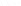
\includegraphics[scale=1.5]{redex.pdf}
\end{center}
that is, an application node whose left child is an abstraction node. In a well-typed $\lambda$-term, we define the \emph{type of a redex} to be the type of the left sub-term of its application node. In the figure above, the type of the redex is $\tau\rightarrow\sigma$. If the abstraction node of a redex is labeled by $\lambda x$, we say that $x$ is the variable of the redex and that it is an \emph{$x$-redex}. 

Let us go back to the proof of Thm.~\ref{prop:one-register}. We proceed by induction on the set of types $S$. The main observation is that, if the evaluation of a redex of type $\sigma\rightarrow \tau$ creates new redexes, then their types are either $\sigma$ or $\tau$, they are in particular in $S\setminus\{\sigma\rightarrow\tau\}$. Thus, we only need to show that the function that evaluates all the redexes of a fixed type is derivable. As we only create strictly smaller redexes, we need to iterate this process only finitely many times, the bound being the size of $S$. 

  Since we have only finitely many typed variables, it is enough to show that the function that evaluates all the redexes of a fixed type $\sigma$ and a fixed variable $x$ is derivable. This will be our goal in the rest of this section.

\begin{proposition}\label{thm:evalOneType}
 For every typed set $X$, every finite set $S$ of simple types and every $x\in X$ and $\sigma\in S$, the function 
    \begin{align*}
        M \in  \LinTerms S X \quad \mapsto \quad  \begin{array}{l}
        \text{The \lambdaterm obtained by reducing all}\\ \text{the $x$-redexes of type $\sigma$ in $M$} 
        \end{array}
    \end{align*}
    is derivable.
\end{proposition}

To show this proposition, we will factorize (via a derivable function) our \lambdaterms into factors satisfying the following properties:
\begin{itemize}
\item All the $x$-redexes of type $\sigma$ fall entirely into one of the factors. In other words, for every such redex, its application node, its abstraction node, and the variable it binds are in the same factor.
\item Each factor have a a very specific shape called \emph{thin}. Those factors, which are \lambdaterms with ports, are roughly speaking those terms whose normal form have the shape of a word (by opposition to trees, which is the general case).
\end{itemize}
Since each redex is fully contained in a thin factor, it is enough to show that normalization of thin \lambdaterms (with ports) is derivable. To do so, we prove that the word obtained by normalizing a thin \lambdaterm results from a depth-first traversal of the later. Using the fact that depth-first traversal is a basic function, we show that normalization of thin $\lambda$-terms is derivable.
 
 The last ingredient to conclude the proof is to notice that $\beta$-reducing the factors of (a factorization of) a $\lambda$-term, then applying a flattening, is the same thing as $\beta$-reducing the original $\lambda$-term, which is a direct consequence from the fact that $\beta$-reduction is a congruence on terms. This concludes the proof. 
 
 In the rest of this section, we develop on each of the two main steps of the proof.  In Sec.~\ref{subsub:thin} we present thin \lambdaterms with ports and show how to normalize them. Then we show in Sec.~\ref{subsub:facto} how to factorize a \lambdaterm into thin factors. 
 

\subsubsection{Evaluation of thin $\lambda$-terms}\label{subsub:thin}

As discussed earlier in the proof sketch, we will need to evaluate \lambdaterms with ports (the factors of our factorization). In the following, we will denote by $\lamrank X$ the ranked set 
\begin{align*}
     \overbrace{\set{x : x \in X}}^{\text{arity 0}} \cup \overbrace{\set{\lambda x : x \in X}}^{\text{arity 1}} \cup  \overbrace{\set @}^{\text{arity 2}}
\end{align*}
Thus, \lambdaterms with ports are the inhabitants of $\tmonad \lamrank X$. Normalization of these terms generalize that of usual \lambdaterms in a straightforward way: the $i$-th port is replaced by a fresh variable $x_i$, the obtained \lambdaterm (without ports) is evaluated as usual, then the variable $x_i$ is replaced back by the port $i$, as one can see in the following example.  
  \begin{center}
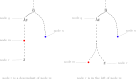
\includegraphics[scale=1.4]{normalization-with-ports.pdf}
\end{center}
  Note that when a \lambdaterm is linear, its normal form has the same number of ports. Note also that respecting the original order of ports in the normal form (which is important for compositionality) may twist ports, as in the example above. As a consequence, normalization of linear \lambdaterms with ports is an arity preserving function of  type:
  \begin{align*}
  \tmonad \lamrank X \to \reduce 1 \tmonad \lamrank X 
  \end{align*}
%Keeping the original order of ports in the normal form (which generates twists) is important for compositionality.
% Indeed, if the ports 1 and 2 of the left-most \lambdaterm of the example above was connected respectively to two terms $u$ and $v$, then its normal form would be 
   
Let us present now the class of \emph{thin \lambdaterms with ports}.
 
\begin{definition}
We say that the node of a $\lambda$-term is \emph{branching} if its has at two distinct children which are not ports.
 
A \emph{thin $\lambda$-term with ports} is a term from $\tmonad \lamrank X$ in which every branching node is the application node of a redex. In the remaining of this section we will omit the mention ``with ports'' if clear from the context.
%We denote by $\thinterm S X$ the set of thin $\lambda$-terms.
\end{definition}

Since thin $\lambda$-terms branch only on redexes, the result of their evaluation is a ``word'', in the sens that every node has at most one non-port child.  We will show that this word can actually be obtained by a depth-first traversal of the original $\lambda$-term. We will then use the basic depth-first traversal  function to show that normalization of thin $\lambda$-terms is derivable. 

The left $\lambda$-term below is linear and thin. The colored nodes are the ones which are not redexes nor the variables of these redexes. The right $\lambda$-term is its normal form: we can see that the order of in which the nodes appear top-down follows the depth-first traversal of the original $\lambda$-term.  
\begin{center}
		\includegraphics[scale=.28]{normalisation-thin}
		\end{center}

\begin{proposition}\label{prop:EvaluateThin}
 For every typed set $X$ and every finite set $S$ of simple types, the function 
    \begin{align*}
    \tmonad \lamrank X &\quad\to\quad \reduce 1 \tmonad \lamrank X\\
        M & \quad \mapsto \quad \text{normal form of $M$ if $M$ is linear and thin}
    \end{align*}
    is derivable.
\end{proposition}

Let $t$ be a strongly thin $\lambda$-term and let $u$ be its normal form. As noticed before, $u$ has the shape of a word. Moreover, since $t$ is linear, the nodes of $u$ are exactly the nodes of $t$ which are not redexes, nor their variables.

\begin{proposition}\label{prop:normal-form-depth-first} Let $t$ be a linear thin \lambdaterm and let $u$ be its normal form. 
The order in which the inner nodes (ie. non ports) of $u$ appear top-down is the depth-first order of $t$.  
\end{proposition}

\begin{proof}
To establish this proposition, we need the following lemma.
\begin{lemma}\label{lem:internalLemma}
Let $t$ be a linear thin $\lambda$-term and let $r$ be one of its redexes. Consider $m$ to be the binder node of $r$ and $n$ to be its variable node.

The node $n$ is the greatest (that is the left-most) node in the sub-term $t|_m$ w.r.t. the depth-first order. 
\end{lemma}

\begin{proof}
We proceed by induction on the length of the path between $m$ and $n$. When it is $0$ the result is clear. Suppose by contradiction that it is strictly greater than $0$ and that there is a node $o$ which is strictly greater than $n$. We take $o$ to be the smallest node which is greater than $n$. Since $t$ is thin, the least common ancestor $l$ between $n$ and $o$ is an application node of a redex. Since $n$ is smaller than $o$, $n$ is the left descendant  of $l$, in other words it is the descendant of the left child $p$
of $l$, which is a binder. The node $m, n, o$ and $p$ are illustrated below:
\begin{center}
		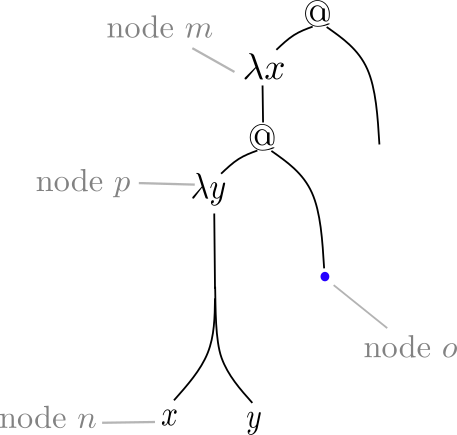
\includegraphics[scale=.4]{lemma-thin.pdf}
\end{center} 
 By induction hypothesis, the variable
bound by $p$ is strictly greater than $n$. Is is also strictly smaller than $o$, which gives a contradiction and concludes the proof. 
\end{proof}

Let us go back to the proof of our proposition. Consider two inner nodes $n, m$ of $t$ which are also nodes of $u$, and such that $m$ is smaller than $n$ is the tree order of $t$. We show that $n$ is a descendant of $m$ in $u$. There is two cases to consider:
\begin{itemize}
\item Either $n$ is a descendant of $m$ in $t$, in this case we can conclude easily since $\beta$-reduction preserves the descendant relation. Indeed, by a small analysis of $\beta$-reduction, one can notice that a reduction step may extend the descendant relation, but can never change (or break) the order of two comparable nodes in the original $\lambda$-term.  
\item  Otherwise, let us consider the lowest common ancestor $p$ of $m$ and $n$. We proceed by induction on the length of the path between $m$ and $p$. By definition of thin $\lambda$-terms, since $p$ is branching it is necessarily an application node, whose left child $q$ is a binder node, let us say $\lambda x$. 
By Lemma~\ref{lem:internalLemma}, $m$ is smaller w.r.t. the depth-first order than the node $r$ of the variable bound by $q$ . 
We are then left with the following two situations. The first case, illustrated by the left figure below, is when $r$ is a descendant of $m$ in $t$. In this case, after one reduction step $n$ will be a descendant of of $m$. The other case is when $m$ is in the left of $r$ in $t$, as illustrated by the right figure below. In this case, after one reduction step, the lowest common ancestor between $m$ and $n$ will be a descendant of $p$, and we can conclude by induction hypothesis. 
\begin{center}
\includegraphics[scale=.4]{cases-lemma}
\end{center}
\end{itemize}
This concludes the proof of the first claim.
%\end{center}    
\end{proof}

Let us construct now a derivable function which computes the normal form of linear thin $\lambda$-terms. We illustrate this construction on the term $t$ below which will be our running example in this proof. 
\begin{center}
\includegraphics[scale=.4]{running-thin}
\end{center}

\begin{proof}[Proof of Proposition~\ref{prop:EvaluateThin}] Let $t$ be a linear thin $\lambda$-term in $\tmonad \lamrank X$.
%Let us show that the evaluation of thin $\lambda$-terms is derivable. We will consider an additional hypothesis on thin $\lambda$-terms:
%\begin{center}
%\textit{If a node is an application node of a redex, then it is branching.}$\qquad\qquad (H)$
%\end{center}
%Hypothesis $(H)$ is the converse of the condition on thin $\lambda$-terms. We will first show that normalization of thin $\lambda$-terms with this additional condition (let us call them strongly thin $\lambda$-terms) is derivable, then we will show later how to get rid of it.



%To establish the second claim, it is enough to show it for one step of $\beta$-reduction. But this last point is clear by a simple analysis of $\beta$-reduction, as far as we consider that the right child of the $@$ node of every redex is not a port. This is is guaranteed by the condition $(H)$ of strongly thin $\lambda$-terms. 

\begin{enumerate}
\item
We start by distinguishing the redexes of $t$ and their variables from the other nodes. For that, we apply the characteristic function of the following first-order query $\varphi$:
    \begin{center}
    ``The node $u$ is a redex or a variable of a redex''
    \end{center}
    This query is first-order expressible. Indeed it is the disjunction of the following queries
$$\begin{array}{rl}
@\mathsf{Redex}(u) = & @(u) \wedge \exists v \ \mathrm{Child}_1(u,v) \wedge \bigvee_{x\in X}\lambda x(v)\\[8pt]
\lambda\mathsf{Redex}(u)=& \lambda x(u) \wedge \exists v \ \mathrm{Child}_1(v,u) \wedge @(v) \\[8pt]
X\mathsf{Redex}(u) = &\bigvee_{x\in X} x(u) \wedge \exists v\ \lambda\mathsf{Redex}(v) \wedge v\ \mathsf{binds}\ u
\end{array}$$
where $@\mathsf{Redex}(u)$ says that $u$ is the application node of a redex, $\lambda\mathsf{Redex}(u)$ says that it is the abstraction node of a redex and $X\mathsf{Redex}(u)$ says that it is the variable of a redex. 
The formula $u\ \mathsf{binds}\ v$, defined below,  is a binary first-order query expressing that the node $u$ is an abstraction node that binds $v$.
 \begin{align*}
 \bigvee_{x\in X} \lambda x(u) \wedge x(v) \wedge u<v\wedge \forall u<w<v\ \neg \lambda x(w)
 \end{align*}

The query $\varphi$ being first-order, its characteristic function is derivable thanks to Proposition~\ref{prop:forat}. 

When we apply this function to $t$, we get a term in $\tmonad(\lamrank X+\lamrank X)$ term below. 
Below is the effect of this first step on our running example. We colored in red the nodes belonging to the first copy of $\lamrank X$, that is the nodes satisfying the query $\varphi$. These nodes are the ones that will disappear in the normal form of $t$. 
\begin{center}
\includegraphics[scale=.4]{running-thin-2}
\end{center}
\item After that, we apply the depth-first traversal function 
\begin{align*}
            \ranked{\preorder : \tmonad (\lamrank X+\lamrank X) \to \reduce 1\tmonad( \lamrank X+\lamrank X + 0 +2)}
\end{align*}
After this step, our initial term becomes
\begin{center}
\includegraphics[scale=.4]{running-thin-3}
\end{center}  
In this term, the nodes of the normal form appear in the right order thanks to Prop.~\ref{prop:normal-form-depth-first}. Now, we only need to get rid of the redexes and the variable nodes that participated in the computation of the normal form (that is the ones colored in red) together with the nodes $\grayball$ and $\grayballbin$ introduced by the depth-first traversal function. 
\item For this purpose, we apply the function 
\begin{align*}
\ranked{\mathsf{Tagg}}: \ranked{\tmonad (X^\lambda+X^\lambda + 0+
2)} \to \ranked{\tmonad (X^\lambda+X^\lambda + 0+2+1) }
\end{align*}
 which adds the unary symbol $1$ as the parent of every node $2$. This function can be easily implemented using the derivable homomorphism function of Example~\ref{ex:morphism}. Then we apply the factorization $\ancfact$
 to separate the symbol $1$ from the others:
 \begin{align*}
 \ranked{\ancfact : \tmonad (X^\lambda+X^\lambda + 0+2+1) \to \tmonad (\tmonad(X^\lambda+X^\lambda + 0+2)+\tmonad 1))}
 \end{align*}
 
 After this step, our example term becomes    
\begin{center}
\includegraphics[scale=.4]{running-thin-4}
\end{center}

\item Now consider the function 
 \begin{align*}
 \ranked{g: \tmonad(X^\lambda+X^\lambda+0+2) \to \reduce 1\tmonad(X^\lambda+X^\lambda+0+2)}
 \end{align*}
 which is the identity function, except for the following finite set of terms for which it is defined in figure~\ref{fig:definition-g}.
\begin{figure*}
\begin{center}
\includegraphics[scale=.4]{function-g}
\end{center}
\caption{Definition of the function $g$.} \label{fig:definition-g}
\end{figure*}
The red elements are those belonging to the first copy of $\lamrank X$.
\smallskip

Now back to our term, we replace the  $\ranked{\tmonad 1}$ factors by the empty term, and to the other factors we apply the function $g$. After that, we apply the function 
\begin{align*}
\ranked{\reduce 1\reduce 1 \Sigma \to \reduce 1\Sigma}
\end{align*}
which untwists two consecutive applications of $\reduce 1$. Doing so, we get a term of type  $$\ranked{\reduce 1\tmonad(X^\lambda+X^\lambda+0+2)}$$ which is  the normal form of $t$. Our running example becomes then
\begin{center}
\includegraphics[scale=.4]{running-thin-5}
\end{center}

\item Note that we obtained the desired term, but not with the desired type. To obtain a term in 
$\ranked{\reduce 1\tmonad{X^\lambda}}$, we get rid of the labels $0+2$ by transforming them respectively into variables and application nodes. The choice of which variables to choose is not important, since the only terms that will actually have $0+2$ in their results are \lambdaterms which are not linear or not thin.
\end{enumerate}
\end{proof}

  



\subsubsection{Factorizing $\lambda$-terms into blocks of thin $\lambda$-terms}\label{subsub:facto}

In a linear $\lambda$-term, we call \emph{full redex} a set of nodes  containing a redex, the node of its variable, together with the set of nodes between them, as illustrated below
\begin{center}
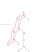
\includegraphics[scale=1.5]{full-redex.pdf}
\end{center}


\begin{proposition}\label{prop:FactoIntoThin} For every finite set of typed variables $X$, for every finite set of types $S$ and for every $x\in X$ and $\sigma\in S$, there is a factorization $$\ranked{f:\tmonad \ranked{X^\lambda} \to \tmonad\tmonad \ranked{X^\lambda}}$$ 
such that for every linear \lambdaterm $t$
\begin{itemize}
\item every full $x$-redex of type $\sigma$ in $t$ is entirely contained in one of the factors of $f(t)$;
\item the factors of $f(t)$ are thin.
\end{itemize}
\end{proposition}

\begin{proof}
We define the function $f$ as the composition of the following three functions
\begin{align*}
\ranked{\tmonad \ranked{X^\lambda} \xrightarrow{\ g\ } \tmonad (\ranked{X^\lambda}+1) \xrightarrow{\ \mathsf{block}^\uparrow\ } \tmonad (\tmonad\ranked{X^\lambda}+\tmonad 1)
\xrightarrow{\ \mathsf{erase}\ } \tmonad \tmonad\ranked{X^\lambda}}
\end{align*}
The function $g$ is a first-order rational tree function, which indicates, using the unary symbol $1$, the places wheres two distinct blocks of $f$ will be separated. We will describe it more precisely a bit later. The function $\mathsf{block}^\uparrow$ will create these blocks and finally, we erase all the factors $\ranked{\tmonad 1}$.

The functions $\mathsf{block}^\uparrow$ is a basic function and  $\mathsf{erase}$ can be easily derivable. 
Let us show how to derive the function $g$, so that the $1$-nodes it introduces creates blocks satisfying the conditions 1 and 2 of Proposition~\ref{prop:FactoIntoThin} (when the input is a linear $\lambda$-term).  

We define $g$ as the composition of the characteristic function of three first-order unary queries: $\mathsf{@redex}, \mathsf{Right}$ and $\mathsf{Left}$, followed by a homomorphims $h$. We define them in the following:
\begin{itemize}
\item The property $\mathsf{@Redex}$ checks whether a node is the application node of an $x$-redex of type $\sigma$. It can be expressed by the following first-order formula, where  $\varphi_\sigma$ is a first-order formula which decides if the type of a node is $\sigma$ (for instance the one given by Lemma~\ref{lem:IsTypeTauFo}):
\begin{align*} \mathsf{App}( u ):=& \mathsf{@}(u)\ \wedge\ \exists v\  \mathrm{Succ}_1(u, v) \wedge \lambda x(v)\ \wedge\ \varphi_\sigma(v)
\end{align*} 
\item The query $\mathsf{Right}$ (resp. $\mathsf{Left}$) checks if the node is an application node, which lies, together with his right (resp. left) child, between the application node of an $x$-redex of type $\sigma$ and the node it binds. Those properties can be easily expressed by a first-order formula.
\end{itemize}

When we apply the characteristic functions of these queries to a term in $\ranked{\tmonad X^\lambda}$, each node will be decorated by three informations: whether is satisfies or not $\mathsf{App}$,  whether is satisfies or not $\mathsf{Right}$ and whether is satisfies or not $\mathsf{Left}$. Note that for linear $\lambda$-terms, some combinations of these properties cannot hold in the same node. For instance, a node cannot satisfy $\mathsf{Right}$ and $\mathsf{Left}$ simultaneously, as this would contradict linearity. 

Now we define the homomorphism $h$, which maps the $\lambda$-terms with these three informations to terms of $\ranked{\tmonad (\ranked{X^\lambda}+1)}$. We define the action of $h$ on each node, depending on its label and the three informations it contains:
\begin{itemize}
\item If the label of the node is $y$ or $\lambda y$ for some variable $y\in X$, or if the label is $@$ and satisfies $\mathsf{App}$, then $h$ returns the same node (seen as a term), forgetting the extra three informations.
\item If the node is an application node satisfying 
\begin{align*}
\neg \mathsf{App} \wedge \neg \mathsf{Right} \wedge\neg \mathsf{Left} 
\end{align*} 
then $h$ adds $1$ to the two children of the node.
\item If the node is an application node satisfying 
\begin{align*}
\neg \mathsf{App} \wedge \neg \mathsf{Right} \qquad\text{(resp. } \neg \mathsf{App} \wedge \neg \mathsf{Left} \text{)}
\end{align*} 
then $h$ adds $1$ to the left (resp. right) child of the node. 
\end{itemize}
Let $t$ be a linear $\lambda$-term. We show that the factors induced by $g$ satisfy the two conditions of Proposition~\ref{prop:FactoIntoThin}. First of all, by analyzing the action of $h$ on each node, note that every application node will receive $1$ as one of its children, except when it is satisfies $\mathsf{App}$. Thus the only branching nodes in a factor are redexes, hence the factors are thin. Now suppose by contradiction that there is some full $x$-redex of type $\sigma$ of $t$ which is not entirely contained in a factor. This means that in $g(t)$ there is a $1$ between the application node of some $x$-redex of type $\sigma$ and its variable.
By construction of $h$, $1$ is the child of an application node (call it $n$). Suppose w.l.o.g. that it is the right child of $n$. The node $n$ cannot satisfy $\mathsf{App}$ because it got $1$ as a child by $h$. Is satisfies $\mathsf{Right}$ by the contradiction hypothesis. Thus its satisfies $\neg \mathsf{App} \wedge \neg \mathsf{Right}$, therefore it receives also $1$ as its left child by $h$. This means that $n$ received $1$ for its both children, and the only way to get that is to satisfy $\neg \mathsf{App} \wedge \neg \mathsf{Right} \wedge\neg \mathsf{Left}$, which gives a contradiction. 
\end{proof}
%\subsubsection{$\beta$-reduction commutes with factorization} \label{subsub:commutes}
%The last ingredient to show Thm.~\ref{thm:evalOneType} is to notice  that factorizing a term, applying some $\beta$-reduction steps to the factors, then flattening, can be simulated by applying  $\beta$-reduction steps directly to the original $\lambda$-term.
%
%Let us state this property more formally. For that, we can generalize the lifting of functions to the lifting of relations as follows. 
%Let $\Sigma$ be a ranked set. If $R\subseteq \ranked{\Sigma}\times\ranked{\Sigma}$ is an arity preserving relation (that is $\arity{u}=\arity{v}$ whenever $(u,v)\in R$), then $R$ can be lifted to $\tmonad R\subseteq \ranked{\tmonad \Sigma} \times \ranked{\tmonad \Sigma}$ in a natural way. 
%
%Since $\beta$-reduction is an arity preserving relation  over linear $\lambda$-terms, its reflexive transitive closure $\beta^*$ is arity preserving as well.  We can lift then the later to $\tmonad \beta^*\subseteq \linterm S X\times\linterm S X$.
%The following proposition is a direct consequence from the fact that $\beta$ is a congruence on terms.
%
%\begin{proposition}\label{prop:betaCommutesWithFacto}
%For every factorization $f:\linterm S X \to \linterm S X$ and every linear $\lambda$-term $M$
%$$\text{if }\qquad f(M) \xrightarrow{\tmonad \beta^*} N \qquad\text{ then }\qquad M\xrightarrow{\beta^*} \flatt(N).$$
%\end{proposition}
%
%

\section{Factorisation forests}

\newcommand{\branches}{\mathsf{B}}

\paragraph{Branches.}
For a ranked set $\rSigma$, define its \emph{branches} to be the unranked set (hence the black font):
\begin{align*}
\branches \rSigma \quad \eqdef \quad \set{(a,i) : a \in \rSigma, i \in \set{1,\ldots,\arity a}}.
\end{align*}
For $a \in  \rSigma$, a branch in $a$ is defined to be any branch obtained by choosing some port of $a$. 
We are mainly interested in the case of branches in terms, which can be visualised as follows:
\mypic{81}
 
For a term, we classify its edges as internal (linking a non-port node with a non-port child) and external (linking a non-port node with a child port). Each edge in a term $t \in \tmonad \rSigma$ corresponds to a branch over $\rSigma$, namely the branch which leads to the edge. Any branch obtained this way is called a \emph{subbranch} of $t$. Here is a picture of subbranches in the case of a term of terms:
\mypic{80} 

\paragraph{Factorisation forests} The idea behind factorisation forests is to split a term into a nested factorisation, which is a term of terms of terms, and so on up to a certain depth.  
Define a \emph{nested factorisation} of depth $k \in \set{1,2,\ldots}$ over alphabet $\rSigma$ to be an element of $\tmonadn k \rSigma$ which is defined by
\begin{align*}
\tmonadn 0 \rSigma = \rSigma  \quad \text{and} \quad \tmonadn {k+1}\rSigma = \tmonad \tmonadn k \rSigma.
\end{align*}
Nested factorisations can be flattened to terms by using an  operation $\flatn k : \tmonadn k \rSigma \rto \tmonad \rSigma $ defined by 
\begin{align*}
     \flatn 1 = \text{\ranked{identity}} \quad \text{and} \quad  \flatn {k+1} \eqdef \flatt  \circ \tmonad \redpar { \flatn k}.
\end{align*}
An equivalent definition of $\flatn {k+1}$ would be $\flatn k \circ \tmonadn {k-1} \flatt$, the equivalence of these definitions corresponds to the fact that $\tmonad$ is a monad.



Branches in  terms $\branches \tmonad \rSigma$  form a semigroup, which we denote by $\branches \rSigma$. 
The idea behind factorisation forests, as expressed in Definition~\ref{def:hom-for} below, is to factorise a term into a term of terms of terms (etc.) so that the depth of nesting is bounded, and at each level all branches behave regularly with respect to some semigroup homomorphism. 

\begin{definition}[Homogeneous factorisations]\label{def:hom-for}
    Let $h : \branches \tmonad \rSigma \to S$ be a semigroup homomorphism.
    \begin{itemize}
\item     We say that $t \in \tmonad \tmonad \rSigma$ is \emph{$h$-homogeneous} if it is either a shallow term (which means that all internal edges originate from the root) or all internal subbranches of $t$ have the same value under $h$.
\item We say that  $t \in \tmonad \rSigma$ is \emph{hereditarily $h$-homogeneous} if it is the unit of some letter;
\item We say that  $t \in \tmonadn k  \rSigma$ is \emph{hereditarily $h$-homogeneous}, for $k \ge 2$, if both:
\begin{enumerate}
    \item  after applying $\tmonad \flatn {k-1}$,   the resulting term in $\tmonad \tmonad \rSigma$ is $h$-homogeneous; and 
    \item every node has a label in $\tmonadn {k-1} \rSigma$ that is hereditarily $h$-homogeneous. 
\end{enumerate}
    \end{itemize}
\end{definition}

The main result of this section is the following version of the factorisation forest theorem. It differs from the original Factorisation Forest Theorem of Imre Simon in the following ways: (a) we consider trees instead of strings; (b) we use aperiodic finite semigroups instead of arbitrary finite semigroups; and (c) the factorisation in the conclusion of the theorem can be computed by a derivable function.  A tree generalisation of the Factorisation Forest Theorem was already proved by Colcombet~\cite[Theorem 1 and Section 3.3]{colcombetCombinatorialTheoremTrees2007}, but Colcombet's result is proved for monadic second-order logic, and therefore it does not satisfy condition (c). 
\begin{theorem}[Factorisation Forest Theorem]\label{thm:factfor}
    Let $\rSigma$ be a finite ranked set and let $h : \branches \rSigma \to M$ be a monoid homomorphism into a finite aperiodic monoid $M$. There is some $k \in \set{1,2,\ldots}$ and a derivable function
    \begin{align*}
        \ranked {f : \tmonad \rSigma \to \tmonad^k \rSigma}  
    \end{align*}
such that $\flatn k \circ \ranked f$ is the identity on $\tmonad \rSigma$, and  all outputs of  $\ranked f$ are hereditarily $h$-homogeneous.
\end{theorem}



\newcommand{\hint}{\bar h}
\newcommand{\hintplus}{\bar h^+}
\newcommand{\branchesplus}{\mathsf B^+}
For $t \in \tmonad  \tmonad \rSigma$ define 
\begin{align*}
    \hint(t) = \set{h(\pi) : \text{$\pi$ is an internal branch of $t$}}
\end{align*}
The theorem is proved by induction on two parameters: the size of $\hint(t)$, and the size of the semigroup generated by $\hint(t)$, ordered lexicographically with the second parameter being more important. This induction is stated in the following lemma, where the theorem is the special case when $A=B=S$. 
\begin{lemma} Let $h : \branchesplus \tmonad \rSigma \to S$ be a semigroup homomorphism into a finite aperiodic semigroup, and let  $A,B \subseteq S$. There is some $k$ and  a derivable function
    \begin{align*}
        \ranked {f_{A,B}: \tmonad \rSigma \to \tmonad^k \rSigma}  
    \end{align*}
    such that $\flatn k \circ \ranked f$ is the identity on $\tmonad \rSigma$, and   outputs of  $\ranked {f_{A,B}}$ are hereditarily $h$-homogeneous for inputs such that:
    \begin{align*}
    B = \hint(t) \qquad A = \text{semigroup generated by $\hint(t)$.}
    \end{align*} 
        
\end{lemma}
The theorem is the special case of the a
\begin{enumerate}
    \item the size of the set 
    \begin{align*}
    \set{h(t)}
    \end{align*}
\end{enumerate}

\begin{itemize}
    \item There is some $x_0 \in $ such that 
    \begin{align}\label{eq:smaller-semigroup}
         \set{ a a_0 :  a \in \hintplus(t)} \subsetneq  \hintplus(t)
    \end{align}
    Choose some $x$ with the above property, and define $T$ to be the above set. It is not hard to see that $T$ is a proper subsemigroup of $S_t$.  Define a \emph{sensitive edge} in $t$ to be any internal edge where the corresponding subbranch has value $x_0$ under  $h$. Let $t' \in \tmonadn 3 \rSigma$ be the nested factorisation that results from $t$ by factorising along sensitive edges. Here is a picture:
    \begin{center}
        picture
    \end{center}
    Define the \emph{outer factorisation} $s \in \tmonad \tmonad \rSigma$ to be the result of applying $\tmonad \flatt$ to $t'$. By definition, every inner subbranch in the outer factorisation ends with $x_0$, and therefore the semigroup generated $\hint(s)$ is contained in 
     by  For a node  $x$ in $t'$ define the \emph{inner factorisation} $s_x \in \tmonad \tmonad \rSigma$ to be the label of node $x$ in $t''$. 
    By definition, the inner factorisations do not have internal subbranches labelled by $a_0$, and therefore 
    \begin{align*}
    \hint(s_x) \subsetneq \hint(t) \qquad \text{for every inner factorisation $s_x$}.
    \end{align*}
    We can therefore use the induction assumption to get nested factorisations for the inner factorisations. 
    For every inner factorisation, its inner subbranches have 
    \begin{itemize}
        \item For every node $x$ in $t'$ its label $t'(x) \in \tmonad \tmonad \rSigma$ satisfies 
        \begin{align*}
        \beta(t'(x)) \subseteq \beta(t) - \set{a_0}.
        \end{align*}
        \item The term $\tmonad \flat (t') \in $ satisfies
        \begin{align*}
            \alpha((\tmonad \flatt)(t')) \subseteq 
        \end{align*}
    \end{itemize}
    
\end{itemize}

For $t \in \tmonad \tmonad \rSigma$ consider $G_t$ the semigroup

% \section{Many registers}

% The following lemma shows that flattening termsand unfolding the matrix power commute. 
% \begin{lemma}
%     The following diagram commutes
% \begin{align*}
%     \ranked{
%         \xymatrix{
%             \tmonad \tmonad (\rSigma^{[k]}) \ar[d]_{\flatt_{\rSigma^{[k]}}} \ar[r]^{\tmonad \unfold_{\rSigma}}&
%             \tmonad ( (\tmonad \rSigma)^{[k]}) \ar[d]^{\unfold_{\tmonad \rSigma}} \\
%             \tmonad ( (\tmonad \rSigma)^{[k]}) \ar[r]^{\unfold_{\tmonad \rSigma}} &
%             (\tmonad \rSigma)^{[k]}
%         }
%     }
% \end{align*}
% \end{lemma} 


\begin{lemma}\label{lem:homo-unfold}
    Let $h : \branches \ranked{\Sigma^{[k]}} \to M$ be the function .
    There is a derivable function 
\begin{align*}
    \ranked{
        \xymatrix{
              \tmonad (\rSigma^{[k]})  \ar[r]^{g} & \rSigma^{[k]} 
        }
    }
\end{align*}
which agrees with unfolding over inputs that are $h$-homogeneous.
\end{lemma}
\begin{proof} Consider an input $t \in \ranked{\tmonad (\Sigma^{[k]})}$ that is $h$-homogeneous. By definition, either $t$ has depth at most two, or there is some 
    \begin{align*}
        m : \set{1,\ldots,k} \to \set{1,\ldots,k}
    \end{align*}
    such that all internal subbranches of $t$ have value $m$ under $h$. In the second case, the function $m$ might be surjective or not. We treat these three cases separately, i.e.~depth two, depth at least three  and $m$ surjective, and depth at most three and $m$ non-surjective.
    \begin{center}
        (todo fill in)
    \end{center}
    % \begin{enumerate}
    %     \item The input has depth at most two. To the input 
    %     \begin{align*}
    %         t \in \ranked{\tmonad (\Sigma^{[k]})}
    %     \end{align*}
    %     apply the function 
    %     \begin{align*}
    %         \tmonad (x \mapsto (x,\ldots,x))
    %     \end{align*}
    %     yielding 
    %     \begin{align*}
    %         t_1 \in \ranked{\tmonad (\Sigma^{[k]})}
    %     \end{align*}
    % \end{enumerate}
\end{proof}





\begin{lemma}
    For every $m \in \set{1,2,\ldots}$ there  is a derivable function $\ranked {g^m}$ such that the  diagram  
\begin{align*}
    \ranked{
        \xymatrix{
            \tmonadn m  (\rSigma^{[k]}) \ar[d]_{\flatn m} \ar[dr]^{g^m}\\
            \tmonad (\rSigma^{[k]})  \ar[r]_{\unfold_\rSigma} &  \rSigma^{[k]}
        }
    }
\end{align*}
commutes for inputs  which are hereditarily $h$-homogeneous.
\end{lemma}
\begin{proof}
Induction on $m$. For $m=1$ we use the function from Lemma~\ref{lem:homo-unfold}. For $m >2$, we define  $\ranked{g^m}$ to be the composition
\begin{align*}
    \ranked{
        \xymatrix{
            \tmonad^m (\rSigma^{[k]}) \ar[r]^{\tmonad g^{m-1}} & 
            \tmonad (\rSigma^{[k]}) \ar[r]^g & 
            \rSigma^{[k]}
            } 
    }
\end{align*}
apply first  $\tmonad \ranked{g^{m-1}}$, yielding  to every label 
\end{proof}

\begin{align*}
    \ranked{
        \xymatrix{ \tmonad (\rSigma^{[k]}) \ar[r]^f \ar[rd]_{id}&
            \tmonadn m  (\rSigma^{[k]}) \ar[d]_{\flatn m} \ar[dr]^{g^m}\\ & 
            \tmonad (\rSigma^{[k]})  \ar[r]_{\unfold_\rSigma} & (\tmonad \rSigma)^{[k]}
        }
    }
\end{align*}


\end{document}
